\documentclass[a4paper,oneside]{book}
%----------------------------------------------------------------------------------------
%	1. GÓI NGÔN NGỮ & FONT
%----------------------------------------------------------------------------------------
\usepackage{iftex}
\ifPDFTeX
  % Chế độ tương thích cho Overleaf khi project vẫn đang dùng pdfLaTeX.
  % mathptmx có kiểu chữ Times gần với Times New Roman, nhưng không phải font
  % Times New Roman hệ thống. Muốn đúng font tuyệt đối, hãy chọn XeLaTeX.
  \usepackage[T5,T1]{fontenc}
  \usepackage{mathptmx}
\else
  \usepackage{fontspec}
  \usepackage{unicode-math}
  \defaultfontfeatures{Ligatures=TeX}
  \IfFontExistsTF{Times New Roman}{%
    \setmainfont{Times New Roman}
    \setsansfont{Times New Roman}
    \setmonofont{Times New Roman}
  }{%
    % Overleaf không cài Times New Roman mặc định vì giấy phép font.
    \setmainfont{TeX Gyre Termes}
    \setsansfont{TeX Gyre Termes}
    \setmonofont{TeX Gyre Termes}
  }
  \IfFontExistsTF{Cambria Math}
    {\setmathfont{Cambria Math}}
    {\setmathfont{TeX Gyre Termes Math}}
\fi
\usepackage[vietnamese]{babel}
\usepackage{indentfirst} % thụt đầu dòng cả đoạn đầu tiên sau tiêu đề (chuẩn VN)
\usepackage{booktabs,tabularx}
\usepackage{algorithm}

%----------------------------------------------------------------------------------------
%	1b. KHẮC PHỤC THƯA CHỮ KHI CĂN LỀ TIẾNG VIỆT
%----------------------------------------------------------------------------------------
% microtype: giãn/co ký tự vi mô để giảm khoảng trắng thưa; emergencystretch cho
% phép TeX nới nhẹ khi không tìm được điểm ngắt tốt; *hyphenmin hạn chế ngắt từ
% quá ngắn (phù hợp tiếng Việt).
\usepackage{microtype}
\emergencystretch=3em
\righthyphenmin=2
\lefthyphenmin=2
%----------------------------------------------------------------------------------------
%	2. CÁC GÓI CƠ BẢN
%----------------------------------------------------------------------------------------
\usepackage{amsmath}
\usepackage{graphicx}
% Hình đã được chuyển sẵn SVG -> PNG (thư mục figures/), dùng \includegraphics
% để tránh gọi Inkscape lúc biên dịch (nguyên nhân timeout trên Overleaf free).
\usepackage{array,booktabs,multirow}
% Cột X căn giữa cho tabularx: bảng luôn vừa \linewidth, nội dung tự xuống dòng
% (dùng cho các bảng số liệu để không tràn lề).
\newcolumntype{Y}{>{\centering\arraybackslash}X}
\usepackage{siunitx} % canh lề số đẹp
\sisetup{
  round-mode=places,round-precision=3,
  table-number-alignment = center,
  detect-weight=true}

\usepackage{subcaption}
\usepackage{float}
\usepackage{setspace}
\usepackage{longtable}
\usepackage{tikz}
\usepackage{ragged2e}
\usetikzlibrary{calc}
\usepackage{etoolbox}

%----------------------------------------------------------------------------------------
%	3. BỐ CỤC & SIÊU LIÊN KẾT
%----------------------------------------------------------------------------------------
\usepackage{geometry}
\geometry{
  a4paper,
  top=20mm,
  bottom=20mm,
  left=30mm,
  right=20mm,
  headheight=15pt,
  headsep=10mm,
  footskip=10mm,
}
% Line spacing ~1.15 (set again after \normalsize in section 7)
\setstretch{1.15}
\definecolor{cobalt}{rgb}{0.0, 0.28, 0.67}
\definecolor{carmine}{rgb}{0.59, 0.0, 0.09}
\usepackage[unicode, colorlinks=false, pdfborder={0 0 0}]{hyperref}

%----------------------------------------------------------------------------------------
%	4. ĐỊNH DẠNG TIÊU ĐỀ (CHƯƠNG, MỤC, CAPTION)
%----------------------------------------------------------------------------------------
\usepackage{titlesec}
\usepackage{caption}
\setcounter{secnumdepth}{3} % đánh số tới \subsubsection  -> 1.3.1
\setcounter{tocdepth}{1}    % mục lục chỉ hiển thị tới \section (gọn, ít phân cấp)

% Định dạng tiêu đề Chương
\titleformat{name=\chapter}[block]
  {\normalfont\fontsize{14pt}{20pt}\bfseries\centering}
  {Chương \thechapter.}{1em}{\MakeUppercase}
\titleformat{name=\chapter,numberless}[block]
  {\normalfont\fontsize{14pt}{20pt}\bfseries\centering}
  {}{0em}{\MakeUppercase}
\titlespacing*{\chapter}{0pt}{-10pt}{14pt}

% Định dạng tiêu đề Section & Subsection
\titleformat{\section}[hang]
  {\normalfont\fontsize{13pt}{15pt}\selectfont\bfseries}
  {\thesection}{1em}{}
\titleformat{\subsection}[hang]
  {\normalfont\fontsize{13pt}{16.5pt}\selectfont\bfseries}
  {\thesubsection}{1em}{}

% Định dạng tiêu đề cho hình, bảng
\captionsetup{font=normalsize, labelfont=bf, labelsep=colon}
\captionsetup[table]{skip=6pt}
\captionsetup[figure]{skip=6pt}
\setlength{\textfloatsep}{12pt plus 2pt minus 2pt}
\setlength{\floatsep}{10pt plus 2pt minus 2pt}
\setlength{\intextsep}{10pt plus 2pt minus 2pt}

%----------------------------------------------------------------------------------------
%	5. ĐỊNH DẠNG MỤC LỤC & CÁC DANH SÁCH
%----------------------------------------------------------------------------------------
\usepackage{tocloft}
\usepackage{textcase} % \MakeTextUppercase - xử lý đúng chữ có dấu tiếng Việt khi in hoa

% Định dạng tiêu đề của các trang danh sách
\makeatletter
\renewcommand{\@cftmaketoctitle}{%
  \clearpage
  {\centering\bfseries\fontsize{14pt}{20pt}\selectfont \MakeTextUppercase{\contentsname}\par}
  \nobreak\vskip 14pt
  {\normalsize\hfill Trang}\par\vskip 4pt
}
\renewcommand{\@cftmakeloftitle}{%
  \clearpage
  {\centering\bfseries\fontsize{14pt}{20pt}\selectfont \MakeTextUppercase{\listfigurename}\par}
  \nobreak\vskip 14pt
}
\renewcommand{\@cftmakelottitle}{%
  \clearpage
  {\centering\bfseries\fontsize{14pt}{20pt}\selectfont \MakeTextUppercase{\listtablename}\par}
  \nobreak\vskip 14pt
}
\makeatother

% Định dạng các dòng trong Mục lục
\renewcommand{\cftchappresnum}{Chương }
\renewcommand{\cftchapaftersnum}{.}
\setlength{\cftchapnumwidth}{8em}
\renewcommand{\cftsecleader}{\cftdotfill{\cftdotsep}}
\renewcommand{\cftsubsecleader}{\cftdotfill{\cftdotsep}}
\renewcommand{\cftdotsep}{3}

% Mục cấp Chương (Chương 1, Lời cam đoan, Kết luận...) — in hoa, in đậm
% Lưu ý: không dùng \renewcommand{\cftchapfont}{\bfseries\MakeUppercase} vì
% cách này chỉ "ăn" 1 ký tự đầu, làm vỡ dấu tiếng Việt — phải ghi đè \l@chapter
% trực tiếp để bọc đúng dấu ngoặc cho \MakeTextUppercase nhận đủ toàn bộ tên chương.
\renewcommand{\cftchapfont}{\bfseries\fontsize{12pt}{14pt}\selectfont}
\renewcommand{\cftchappagefont}{\bfseries\fontsize{12pt}{14pt}\selectfont}
\renewcommand{\cftchapleader}{\cftdotfill{\cftdotsep}}

\makeatletter
\renewcommand*{\l@chapter}[2]{%
  \ifnum \c@tocdepth >\m@ne
    \addpenalty{-\@highpenalty}%
    \vskip \cftbeforechapskip
    {\leftskip \cftchapindent\relax
     \rightskip \@tocrmarg
     \parfillskip -\rightskip
     \parindent \cftchapindent\relax\@afterindenttrue
     \interlinepenalty\@M
     \leavevmode
     \@tempdima \cftchapnumwidth\relax
     \let\@cftbsnum \cftchappresnum
     \let\@cftasnum \cftchapaftersnum
     \let\@cftasnumb \cftchapaftersnumb
     \advance\leftskip \@tempdima \null\nobreak\hskip -\leftskip
     {\cftchapfont \MakeTextUppercase{#1}}\nobreak
     \cftchapfillnum{#2}}%
  \fi}%
\makeatother

% Mục cấp 1.1 (section) — chỉ in đậm, không in hoa
\renewcommand{\cftsecfont}{\bfseries}
\renewcommand{\cftsecpagefont}{\bfseries}

% Rút gọn mục lục: chỉ hiển thị tới cấp \section (Chương + 1.1), ẩn các mục
% con \subsection/\subsubsection. Do titlesec ghi mọi cấp vào .toc bất kể
% \tocdepth, ta ẩn ngay lúc ĐỌC lại .toc bằng cách vô hiệu \l@subsection.
\makeatletter
\renewcommand*{\l@subsection}[2]{}
\renewcommand*{\l@subsubsection}[2]{}
\makeatother

% Làm đều khoảng cách các dòng trong Mục lục
\setlength{\cftbeforechapskip}{\parskip}
\setlength{\cftbeforesecskip}{\parskip}
\setlength{\cftbeforesubsecskip}{\parskip}

%----------------------------------------------------------------------------------------
%	6. CÁC GÓI MỞ RỘNG (CODE, GIẢI THUẬT)
%----------------------------------------------------------------------------------------
\usepackage{algorithm}
\usepackage{algpseudocode}
\makeatletter
\renewcommand{\ALG@name}{Giải thuật}
\renewcommand{\listalgorithmname}{Danh sách giải thuật}
\makeatother

\usepackage{listings}
\usepackage{xcolor}
\lstset{
  language=C++,
  basicstyle=\ttfamily\footnotesize,
  keywordstyle=\color{blue}\bfseries,
  stringstyle=\color{red},
  commentstyle=\color{green!50!black}\itshape,
  breaklines=true,
  frame=single,
  numbers=left,
  numberstyle=\tiny\color{gray},
  tabsize=2
}

%----------------------------------------------------------------------------------------
%	7. FONT CHUNG & KHOẢNG CÁCH ĐOẠN
%----------------------------------------------------------------------------------------
\makeatletter
\renewcommand\normalsize{%
  \@setfontsize\normalsize{13pt}{17.55pt}%
  \abovedisplayskip 6pt plus 2pt minus 2pt
  \abovedisplayshortskip \z@ plus 2pt
  \belowdisplayshortskip 6pt plus 2pt minus 2pt
  \belowdisplayskip \abovedisplayskip
}
\makeatother
\normalsize
\setlength{\parskip}{3pt}
\setlength{\parindent}{15pt}

\renewcommand{\cftfigpresnum}{Hình~}
\setlength{\cftfignumwidth}{6.0em}

\renewcommand{\cfttabpresnum}{Bảng~}
\setlength{\cfttabnumwidth}{6.0em}

\usepackage{thesis}
\usepackage{setspace}

\cftsetpnumwidth{2em}
\cftsetrmarg{3em}
\setlength{\cftsecnumwidth}{3em}
\setlength{\cftsubsecnumwidth}{4em}

\setstretch{1.15}

%----------------------------------------------------------------------------------------
%	8. TÀI LIỆU THAM KHẢO
%----------------------------------------------------------------------------------------
%  "Tài liệu tham khảo" — không hiện header phải
\fancypagestyle{reflist}{%
  \fancyhf{}
  \fancyhead[L]{\fontsize{12pt}{14pt}\itshape\selectfont \makebox[\textwidth][l]{\datn}}
  \fancyfoot[L]{\fontsize{12pt}{14pt}\itshape\selectfont \nhomten}
  \fancyfoot[R]{\fontsize{12pt}{14pt}\selectfont \thepage}
  \renewcommand{\footrulewidth}{0.4pt}
}


\makeatletter
\patchcmd{\thebibliography}
  {\@mkboth{\MakeUppercase\bibname}{\MakeUppercase\bibname}}
  {\@mkboth{\MakeTextUppercase{\bibname}}{\MakeTextUppercase{\bibname}}\thispagestyle{reflist}}
  {}{}
\apptocmd{\thebibliography}{%
  \RaggedRight
  \sloppy
  \setlength{\itemsep}{3pt}%
  \setlength{\parsep}{0pt}%
}{}{}
\makeatother

\begin{document}
\frontmatter
\pagenumbering{roman}

% --- Bìa ngoài ---
\coverpage
% --- Bìa đệm (copy nguyên bìa chính) ---
\coverpageinner

% --- Mục lục ---
\cleardoublepage
\begin{spacing}{1.15}
\tableofcontents
\end{spacing}

% --- Lời cảm ơn ---
\begin{acknowledgments}
\setlength{\parskip}{4pt}
Để hoàn thành báo cáo đồ án tốt nghiệp này, chúng em đã nhận được sự quan tâm, giúp đỡ và động viên từ gia đình, thầy cô và bạn bè. Những hỗ trợ đó đã giúp nhóm duy trì tiến độ, giữ kỷ luật làm việc và hoàn thành đúng phạm vi nghiên cứu đã cam kết. Chúng em xin ghi nhận và trân trọng mọi góp ý trong quá trình thực hiện.

Trước hết, chúng em xin gửi lời cảm ơn chân thành đến thầy \textbf{\supervisor}, người đã tận tình hướng dẫn, phản biện sâu sắc về tính độc lập của thực nghiệm và định hướng cho nhóm nâng cấp hệ thống từ quy mô thực tập lên đồ án tốt nghiệp hoàn chỉnh: bổ sung kiểm thử đối kháng trực tiếp bằng công cụ độc lập (\texttt{garak}, \texttt{PyRIT}), đánh giá trên benchmark công khai ngoài phân phối (\texttt{deepset/prompt-injections}), đo đạc đầy đủ phân vị độ trễ (\texttt{p50/p95/p99}) và đối sánh định lượng công bằng với các giải pháp chuẩn (\texttt{Meta Llama Guard~3}, \texttt{NVIDIA NeMo Guardrails}), đồng thời mở rộng kiến trúc sang bảo vệ truy vấn cơ sở dữ liệu Text-to-SQL và Multi-Tool Agent.

Chúng em xin trân trọng cảm ơn các thầy cô trong \faculty, Học viện Công nghệ Bưu chính Viễn thông, đã truyền đạt kiến thức nền tảng, tạo điều kiện để nhóm tiếp cận các vấn đề an toàn hệ thống LLM/RAG. Những nội dung học phần về an toàn thông tin, phát triển phần mềm và phương pháp nghiên cứu là nền tảng để nhóm thiết kế, hiện thực và kiểm thử khung guardrail. Chúng em cũng cảm ơn các ý kiến phản biện của hội đồng trong quá trình rà soát tiến độ.

Cuối cùng, chúng em cảm ơn gia đình và bạn bè đã đồng hành trong suốt thời gian thực hiện đồ án tốt nghiệp. Sự động viên tinh thần và chia sẻ về mặt thời gian đã giúp nhóm duy trì nhịp làm việc ổn định khi chạy đánh giá, chỉnh sửa báo cáo và hoàn thiện minh chứng. Báo cáo chắc chắn vẫn còn những giới hạn trong phạm vi phòng thí nghiệm; chúng em rất mong nhận được góp ý của quý thầy cô hội đồng chấm đồ án để tiếp tục hoàn thiện.

Chúng em xin chân thành cảm ơn!

\vspace{0.3cm}
\begin{flushright}
    \textit{TPHCM, ngày 22 tháng 11 năm \yearsubmit} \\
    \makebox[8cm][c]{\textbf{ĐẠI DIỆN NHÓM SINH VIÊN}} \\
    \makebox[8cm][c]{\textit{(Ký và ghi rõ họ tên)}} \\[0.85cm]
    \makebox[8cm][c]{\textbf{\studentname} --- \textbf{\studentnametwo}}\\
\end{flushright}
\end{acknowledgments}


% --- Thuật ngữ và từ viết tắt ---
% --- DANH MỤC KÝ HIỆU VÀ CHỮ VIẾT TẮT (BẢNG THỦ CÔNG) ---
% Sắp xếp theo thứ tự chữ cái A, B, C... của cột "Từ viết tắt", theo đúng yêu cầu
% mục II.4 của văn bản gốc PTIT (xem docs/report/report-compliance-audit.md mục C06).

\chapter*{Danh mục ký hiệu và chữ viết tắt}
\addcontentsline{toc}{chapter}{Danh mục ký hiệu và chữ viết tắt}
% \chapter* không tự gọi \markboth -- set thủ công để Header phải hiển thị đúng
% (xem docs/report/report-compliance-audit.md mục C12).
\markboth{DANH MỤC KÝ HIỆU VÀ CHỮ VIẾT TẮT}{}
\singlespacing

% raggedright ở cột nghĩa để tránh giãn chữ (khoảng trắng thưa) khi căn đều
\begin{longtable}{p{0.15\linewidth} >{\raggedright\arraybackslash}p{0.4\linewidth} >{\raggedright\arraybackslash}p{0.35\linewidth}}
\toprule
\bfseries Từ viết tắt & \bfseries Nghĩa tiếng Anh & \bfseries Nghĩa tiếng Việt \\
\midrule
\endhead
\bottomrule
\endfoot
AI & Artificial Intelligence & Trí tuệ nhân tạo \\
\addlinespace
API & Application Programming Interface & Giao diện lập trình ứng dụng \\
\addlinespace
ASR & Attack Success Rate & Tỉ lệ tấn công thành công \\
\addlinespace
AST & Abstract Syntax Tree & Cây cú pháp trừu tượng \\
\addlinespace
BM25 & Best Matching 25 & Thuật toán xếp hạng tìm kiếm theo từ khóa \\
\addlinespace
DATN & Đồ án tốt nghiệp & Đồ án tốt nghiệp đại học \\
\addlinespace
DLP & Data Loss Prevention & Ngăn chặn rò rỉ dữ liệu \\
\addlinespace
FAQ & Frequently Asked Questions & Câu hỏi thường gặp \\
\addlinespace
FNR & False Negative Rate & Tỉ lệ âm tính giả \\
\addlinespace
FPR & False Positive Rate & Tỉ lệ dương tính giả \\
\addlinespace
FR & Functional Requirement & Yêu cầu chức năng \\
\addlinespace
FTS5 & Full-Text Search 5 & Mô-đun tìm kiếm toàn văn của SQLite \\
\addlinespace
HR & Human Resources & Nhân sự \\
\addlinespace
IT & Information Technology & Công nghệ thông tin \\
\addlinespace
JSON/JSONL & JavaScript Object Notation (Lines) & Định dạng dữ liệu dùng cho log \\
\addlinespace
LLM & Large Language Model & Mô hình ngôn ngữ lớn \\
\addlinespace
LLMSVS & LLM Security Verification Standard & Chuẩn xác minh bảo mật cho LLM (của OWASP) \\
\addlinespace
MVP & Minimum Viable Product & Sản phẩm khả dụng tối thiểu \\
\addlinespace
NFR & Non-Functional Requirement & Yêu cầu phi chức năng \\
\addlinespace
OWASP & Open Worldwide Application Security Project & Tổ chức phi lợi nhuận về bảo mật ứng dụng \\
\addlinespace
P2SQL & Prompt-to-SQL Injection & Tấn công tiêm nhiễm từ ngôn ngữ tự nhiên sang truy vấn SQL \\
\addlinespace
PII & Personally Identifiable Information & Thông tin định danh cá nhân \\
\addlinespace
PoC & Proof of Concept & Bằng chứng khái niệm (thử nghiệm khả thi) \\
\addlinespace
PTIT & Posts and Telecommunications Institute of Technology & Học viện Công nghệ Bưu chính Viễn thông \\
\addlinespace
RAG & Retrieval-Augmented Generation & Sinh văn bản có truy hồi tri thức \\
\addlinespace
RBAC & Role-Based Access Control & Kiểm soát truy cập dựa trên vai trò \\
\addlinespace
SIEM & Security Information and Event Management & Hệ thống quản lý sự kiện và thông tin bảo mật \\
\addlinespace
STRIDE & Spoofing, Tampering, Repudiation, Information Disclosure, Denial of Service, Elevation of Privilege & Mô hình phân loại mối đe dọa bảo mật \\
\addlinespace
TPR & True Positive Rate & Tỉ lệ phát hiện đúng (độ nhạy / Recall) \\
\addlinespace
UI & User Interface & Giao diện người dùng \\

\end{longtable}


% --- Danh mục bảng ---
\cleardoublepage
\phantomsection
\addcontentsline{toc}{chapter}{Danh mục các bảng vẽ}
\chapter*{DANH MỤC CÁC BẢNG VẼ}
\begingroup
\singlespacing
\makeatletter
\@starttoc{lot}
\makeatother
\endgroup

% --- Danh mục hình ---
\cleardoublepage
\phantomsection
\addcontentsline{toc}{chapter}{Danh mục các hình vẽ, sơ đồ}
\chapter*{DANH MỤC CÁC HÌNH VẼ, SƠ ĐỒ}
\begingroup
\singlespacing
\makeatletter
\@starttoc{lof}
\makeatother
\endgroup

% --- Kế hoạch thực hiện công việc nhóm ---
\cleardoublepage
\chapter*{Bảng phân công nhiệm vụ nhóm thực hiện}
\addcontentsline{toc}{chapter}{Bảng phân công nhiệm vụ nhóm thực hiện}
\markboth{BẢNG PHÂN CÔNG NHIỆM VỤ NHÓM THỰC HIỆN}{}
\setlength{\parskip}{4pt}

Bảng~\ref{tab:ke-hoach-nhom} và Bảng~\ref{tab:doi-chieu-nhiem-vu} trình bày kế hoạch phân công công việc giữa hai thành viên (\textbf{SV1} --- \studentname{}, Nhóm trưởng; \textbf{SV2} --- \studentnametwo{}) cùng bảng đối chiếu 11 hạng mục nhiệm vụ đề tài (5 nội dung lý thuyết và 6 nội dung thực hành do Giáo viên hướng dẫn giao) với các chương, mục và minh chứng thực nghiệm trong quyển báo cáo.

\begin{table}[!htbp]
\centering
\caption{Kế hoạch và phân công thực hiện công việc của nhóm Thanh\_01 (A06)}
\label{tab:ke-hoach-nhom}
\small
\setlength{\tabcolsep}{4pt}
\begin{tabularx}{\linewidth}{@{}C{0.05\linewidth}X C{0.12\linewidth}C{0.14\linewidth}@{}}
\toprule
\textbf{TT} & \textbf{Nội dung công việc} & \textbf{Phụ trách} & \textbf{Mức độ} \\
\midrule
1 & Khảo sát kiến trúc RAG, bề mặt tấn công OWASP LLM Top~10, nguyên tắc fail-closed và các giải pháp Llama Guard~3, NeMo Guardrails, garak, PyRIT & Cả hai & Hoàn thành \\
2 & Phân tích yêu cầu FR/NFR, mô hình mối đe doạ, thiết kế kiến trúc Guardrails đa lớp (đầu vào $\rightarrow$ truy hồi $\rightarrow$ ngữ cảnh $\rightarrow$ đầu ra) & Cả hai & Hoàn thành \\
3 & Xây dựng FastAPI Security Gateway, chuỗi Guard (Input + Pre-decoder, RAG Context, Output/DLP) và truy hồi lai BM25 + Dense + Pre-retrieval RBAC & SV1 & Hoàn thành \\
4 & Tách và khóa SHA-256 tập holdout, tích hợp benchmark công khai \texttt{deepset/\allowbreak prompt-injections} ($662$ mẫu) và bộ kiểm thử nội bộ ($425$ mẫu) & SV1 & Hoàn thành \\
5 & Thực nghiệm đối chứng có/không có Guardrails, đo phân vị độ trễ \texttt{p50/p95/p99} từng lớp và tổng thể (tối ưu \texttt{think=False} cho Semantic Judge) & SV1 & Hoàn thành \\
6 & Kiểm thử đối kháng bằng \texttt{NVIDIA garak v0.17.1} ($2.048$ probe), \texttt{PyRIT} và lập bảng đối sánh với \texttt{Llama Guard~3 1B} \& \texttt{NeMo Guardrails} & SV1 & Hoàn thành \\
7 & Mở rộng kho dữ liệu doanh nghiệp Nhà Mộc Việt (12 bảng SQL, 29 tài liệu) và Multi-Tool Company Agent (Approval Queue) & SV2 & Hoàn thành \\
8 & Xây dựng Text-to-SQL Guard (SQLite \texttt{EXPLAIN} + Authorizer AST) và Indirect Data-Cell Result Guard ($100\%$ holdout) & SV2 & Hoàn thành \\
9 & Kiểm thử tự động tích hợp ($469$ unit/integration tests PASS) và phân tích các hạn chế về tính hợp lệ thực nghiệm & Cả hai & Hoàn thành \\
10 & Soạn thảo và hoàn thiện quyển báo cáo Đồ án tốt nghiệp theo QĐ~449/QĐ-HV & Cả hai & Hoàn thành \\
\bottomrule
\end{tabularx}
\end{table}

\textbf{Nguyên tắc làm việc:} hai thành viên rà soát chéo kết quả của nhau trước khi hợp nhất; mọi số liệu đánh giá bám sát artifact/script tái lập được; không mở rộng kết luận vượt quá bằng chứng thực nghiệm.

\begin{table}[!htbp]
\centering
\caption{Đối chiếu 11 hạng mục Lý thuyết và Thực hành được giao với nội dung báo cáo}
\label{tab:doi-chieu-nhiem-vu}
\footnotesize
\setlength{\tabcolsep}{3.5pt}
\begin{tabularx}{\linewidth}{@{}C{0.06\linewidth}L{0.42\linewidth}L{0.18\linewidth}X@{}}
\toprule
\textbf{Mã} & \textbf{Nội dung nhiệm vụ theo bảng giao đề tài} & \textbf{Vị trí trong báo cáo} & \textbf{Kết quả / Minh chứng đạt được} \\
\midrule
\textbf{LT1} & Tổng quan kiến trúc RAG và bề mặt tấn công runtime (Direct/Indirect Prompt Injection, đầu độc ngữ cảnh, rò rỉ dữ liệu theo OWASP LLM Top~10) & Chương~1 (Mục~1.1, 1.2) & Phân tích 4 bề mặt tấn công liên thông và ánh xạ chi tiết OWASP LLM01, LLM02, LLM06, LLM08. \\
\textbf{LT2} & Kiến trúc Guardrails đa lớp theo nguyên tắc fail-closed: kiểm duyệt đầu vào, kiểm soát truy cập trước truy hồi, làm sạch ngữ cảnh, lọc đầu ra & Chương~1 (Mục~1.3), Chương~2 (Mục~2.1--2.4) & Thiết kế chuỗi phòng thủ chiều sâu fail-closed kết hợp Pre-retrieval RBAC và SQLite Authorizer AST. \\
\textbf{LT3} & Khảo sát giải pháp Guardrails mã nguồn mở (Llama Guard, NeMo Guardrails) và bộ dữ liệu tấn công công khai & Chương~1 (Mục~1.4, 1.5, Bảng~1.1) & Phân tích cơ chế Llama Guard~3 1B, NeMo \texttt{self\_\allowbreak check\_\allowbreak input} và bộ dữ liệu \texttt{deepset/\allowbreak prompt-injections} ($662$ mẫu). \\
\textbf{LT4} & Tìm hiểu khung kiểm thử đối kháng tự động và quy trình kiểm thử hộp đen cho ứng dụng LLM & Chương~1 (Mục~1.4, 1.5), Chương~4 (Mục~4.6) & Khảo sát kiến trúc probe của \texttt{NVIDIA garak v0.17.1} và Converter/\allowbreak Orchestrator của \texttt{Microsoft PyRIT}. \\
\textbf{LT5} & Phương pháp đánh giá định lượng: tách tập tinh chỉnh luật và tập kiểm định độc lập, chỉ số TPR, FPR, độ trễ p50/p95, đánh đổi an toàn -- khả dụng & Chương~2 (Mục~2.2), Chương~4 (Mục~4.1) & Định nghĩa giao thức tách dev/holdout khóa SHA-256 và bộ chỉ số $\text{TPR}$, $\text{FPR}$, $\text{F1}$, $\text{ASR}$, $\text{p50/p95/p99}$. \\
\midrule
\textbf{TH1} & Xây dựng chatbot RAG doanh nghiệp mô phỏng chứa dữ liệu nhạy cảm giả lập, cung cấp cổng truy cập (gateway) phục vụ kiểm thử & Chương~2 (Mục~2.3), Chương~3 (Mục~3.1, 3.3) & Kho RAG 48 văn bản đa phòng ban + CSDL Nhà Mộc Việt (12 bảng SQL, 29 tài liệu) qua FastAPI Security Gateway. \\
\textbf{TH2} & Triển khai lớp Guardrails đa lớp theo luồng đầu vào $\rightarrow$ truy hồi $\rightarrow$ ngữ cảnh $\rightarrow$ đầu ra, áp dụng nguyên tắc fail-closed & Chương~3 (Mục~3.1--3.3) & Hiện thực Pre-decoder + Input Guard $\rightarrow$ RBAC / SQL AST $\rightarrow$ RAG Context / Result Guard $\rightarrow$ Output/DLP Guard ($469$ tests PASS). \\
\textbf{TH3} & Xây dựng bộ kiểm thử kết hợp dữ liệu công khai và kịch bản tự xây; tách và khóa tập holdout trước khi tinh chỉnh luật & Chương~4 (Mục~4.1, 4.4, 4.7) & Khóa SHA-256 tập \texttt{v2\_\allowbreak holdout} ($50$ mẫu), \texttt{sql\_\allowbreak holdout} ($14$ mẫu), kết hợp \texttt{v3\_425} và \texttt{deepset} công khai ($662$ mẫu). \\
\textbf{TH4} & Thực nghiệm đối chứng giữa cấu hình có và không có Guardrails trên cùng kho tài liệu & Chương~4 (Mục~4.2, Bảng~4.1, 4.2) & Không Guard: $\text{ASR}=84{,}00\%$; Có Guard: $\text{ASR}=0{,}00\%$, kèm ma trận Ablation 8 cấu hình trên cùng kho tài liệu. \\
\textbf{TH5} & Đo và phân tích tỷ lệ chặn thành công, False Positive và độ trễ p50/p95 ở mức tổng thể lẫn từng lớp & Chương~4 (Mục~4.3--4.5, Bảng~4.3, Hình~4.1) & Guard tất định: $\text{p50}=0{,}42\,\text{ms}$, $\text{p95}=1{,}21\,\text{ms}$; Bật Judge (\texttt{think=False}): Judge $\text{p50}=99{,}79\,\text{ms}$, tổng thể $\text{p50}=0{,}73\,\text{ms}$. \\
\textbf{TH6} & Lập bảng đối sánh định lượng với Llama Guard và NeMo Guardrails trên cùng bộ kiểm thử và phần cứng; phân tích kết quả và hạn chế thực nghiệm & Chương~4 (Mục~4.4, 4.9, Bảng~4.4, Hình~4.2) & Trên \texttt{deepset} ($662$ mẫu): Shield AI đạt $\text{F1}=92{,}9\%$ ($\text{FPR}=0{,}5\%$), vượt Llama Guard~3 ($\text{F1}=36{,}9\%$) và NeMo ($\text{F1}=45{,}2\%$); phân tích 4 nhóm hạn chế thực nghiệm (Mục~4.9). \\
\bottomrule
\end{tabularx}
\end{table}


% --- Phần nội dung chính ---
\mainmatter
\pagenumbering{arabic}
\chapter*{Mở đầu}
\addcontentsline{toc}{chapter}{Mở đầu}
\markboth{MỞ ĐẦU}{}

\section*{Lý do chọn đề tài}

Trong những năm gần đây, mô hình ngôn ngữ lớn (Large Language Model --- LLM) được tích hợp ngày càng sâu vào các hệ thống truy vấn tri thức doanh nghiệp, trợ lý tra cứu cơ sở dữ liệu (Text-to-SQL), tác tử đa công cụ (Multi-Tool Agent) và kiến trúc sinh văn bản tăng cường truy hồi (Retrieval-Augmented Generation --- RAG). Lợi ích về khả năng hiểu ngôn ngữ tự nhiên đi kèm các rủi ro an toàn đặc thù tại thời điểm chạy (runtime): tấn công chèn chỉ dẫn trực tiếp (direct prompt injection), tiêm nhiễm gián tiếp qua tài liệu hoặc ô dữ liệu trong cơ sở dữ liệu (indirect prompt/SQL injection), lạm dụng công cụ (tool misuse) và rò rỉ dữ liệu nhạy cảm. Việc chỉ dựa vào khả năng ``tự căn chỉnh'' (alignment) của mô hình hoặc chỉ kiểm thử khép kín trên tập dữ liệu tự sinh là không đủ; một cơ chế phòng thủ thực tiễn đòi hỏi kiến trúc nhiều lớp theo chiều sâu (defense-in-depth), kiểm soát truy cập trước truy hồi, đồng thời phải được kiểm chứng độc lập bằng các bộ dữ liệu công khai, công cụ red-team chuẩn và đo đạc chi phí độ trễ định lượng.

\section*{Bối cảnh và vấn đề}

Hệ thống RAG và Agent doanh nghiệp kết hợp kho tài liệu không cấu trúc với cơ sở dữ liệu có cấu trúc (SQL) và các công cụ thực thi (gửi email, tạo phiếu yêu cầu), tạo ra bốn bề mặt tấn công liên thông: (1)~đầu vào người dùng cố ghi đè chỉ dẫn hệ thống hoặc mã hoá payload qua Base64/ROT13/Leetspeak; (2)~tài liệu trong kho tri thức hoặc ô văn bản trong bảng SQL bị đầu độc chỉ thị ẩn; (3)~câu lệnh SQL do mô hình sinh ra cố vượt quyền đọc bảng/cột nhạy cảm; và (4)~đầu ra mô hình vô tình phát tán bí mật, PII hoặc liên kết thất thoát dữ liệu. Bên cạnh đó, hạn chế phổ biến của nhiều nghiên cứu quy mô phòng thí nghiệm là tình trạng \emph{đánh giá khép kín} (tự sinh mẫu tấn công, tự viết luật regex, tự chấm điểm), thiếu đo đạc phân vị độ trễ (\texttt{p50/\allowbreak p95/\allowbreak p99}) và thiếu đối sánh định lượng với các giải pháp chuẩn quốc tế như Meta Llama Guard~3 hay NVIDIA NeMo Guardrails. Đề tài Đồ án tốt nghiệp này giải quyết trực diện các khoảng trống đó.

\section*{Mục tiêu}

\begin{enumerate}
    \item Nghiên cứu toàn diện bề mặt tấn công của hệ thống RAG, Text-to-SQL và Multi-Tool Agent theo khung OWASP Top~10 for LLM Applications; khảo sát và phân tích cơ chế của các giải pháp phòng thủ chuẩn (\texttt{Llama Guard~3}, \texttt{NeMo Guardrails}) cùng các khung kiểm thử đối kháng độc lập (\texttt{NVIDIA garak}, \texttt{Microsoft PyRIT}).
    \item Thiết kế và hiện thực khung bảo mật đa lớp \textbf{Shield AI}: kết hợp tầng tiền giải mã (\emph{Payload De-obfuscation Pre-decoder} cho Base64/ROT13/Leetspeak/Unicode), chuỗi Guard tất định (Input Guard, Provenance Guard, RAG Context Guard, Output/DLP Guard), bộ phán đoán ngữ nghĩa cục bộ (\emph{Semantic Judge} \texttt{gemma4:e2b-\allowbreak it-\allowbreak q4\_\allowbreak K\_\allowbreak M}) và cơ chế kiểm soát truy cập theo vai trò (\emph{Pre-retrieval RBAC}) trên nền truy hồi lai vectorized.
    \item Mở rộng kiến trúc bảo vệ sang dữ liệu có cấu trúc và tác tử đa công cụ: xây dựng \textbf{SQL Guard} dùng chính trình biên dịch \texttt{EXPLAIN} và \texttt{Authorizer AST callback} của SQLite để kiểm soát quyền truy cập tới từng bảng/cột, \textbf{Indirect Result Guard} quét ô dữ liệu trả về từ CSDL, và \textbf{Multi-Tool Company Agent} có hàng chờ phê duyệt cấp quản lý (\emph{Leader Approval Queue}).
    \item Thực hiện chương trình kiểm thử đối kháng và đánh giá đối sánh độc lập theo bốn trục: (i)~đánh giá trên benchmark công khai ngoài phân phối \texttt{deepset/\allowbreak prompt-\allowbreak injections} ($662$ mẫu đa ngôn ngữ); (ii)~bắn trực tiếp công cụ \texttt{NVIDIA garak v0.\allowbreak 17.\allowbreak 1} ($2.048$ probe qua HTTP REST) và bộ biến đổi/tấn công thích nghi đa lượt \texttt{PyRIT} vào endpoint hệ thống; (iii)~đo đạc chi tiết phân vị độ trễ \texttt{p50/\allowbreak p95/\allowbreak p99} của từng tầng xử lý khi bật/tắt Semantic Judge; và (iv)~lập bảng đối sánh định lượng công bằng với \texttt{Meta Llama Guard~3 1B} và \texttt{NVIDIA NeMo Guardrails}.
\end{enumerate}

\section*{Đối tượng và phạm vi}

\textbf{Đối tượng} nghiên cứu là kiến trúc Guardrails đa lớp kết hợp kiểm soát truy cập RBAC cho hệ thống RAG, Text-to-SQL và Multi-Tool Agent, cùng phương pháp luận kiểm thử đối kháng độc lập và đánh giá đối sánh định lượng. \textbf{Phạm vi} thực nghiệm sử dụng bộ dữ liệu doanh nghiệp tổng hợp đa phòng ban (gồm kho tri thức 48 tài liệu của hệ thống RAG và cơ sở dữ liệu 12 bảng / 29 tài liệu của doanh nghiệp nội thất Nhà Mộc Việt), kết hợp với bộ benchmark công khai \texttt{deepset/\allowbreak prompt-\allowbreak injections} từ HuggingFace và bộ probe gốc của \texttt{garak v0.\allowbreak 17.\allowbreak 1}; toàn bộ suy luận LLM và Semantic Judge chạy cục bộ qua \texttt{Ollama} trên GPU cá nhân (RTX~4050 6\,GB VRAM) để đảm bảo tính tái lập 100\% và không phát sinh chi phí API thương mại.

\section*{Câu hỏi nghiên cứu}

Chương trình thực nghiệm của đồ án (Chương~4) được thiết kế để trả lời năm câu hỏi nghiên cứu định lượng:

\begin{itemize}
    \item \textbf{CH1 (Độ chính xác và khái quát hoá ngoài phân phối).} Bộ luật tất định đạt hiệu quả như thế nào trên tập kiểm thử nội bộ ($425$ case) so với khi kiểm chứng độc lập trên benchmark công khai ngoài phân phối \texttt{deepset/\allowbreak prompt-\allowbreak injections} ($662$ mẫu đa ngôn ngữ), và việc bổ sung tầng tiền giải mã (\emph{Pre-decoder}) cùng luật cấu trúc đa ngôn ngữ cải thiện khả năng khái quát hoá ra sao mà vẫn giữ $\text{FPR} \approx 0\%$?
    \item \textbf{CH2 (Đối sánh với giải pháp chuẩn quốc tế).} Khi chạy trên cùng tập kiểm thử và cùng phần cứng cục bộ, kiến trúc lai của \textbf{Shield AI} (Rule + Pre-decoder + Semantic Judge \texttt{gemma4:e2b}) đạt chỉ số $\text{TPR}$, $\text{FPR}$, $\text{F1}$ và độ trễ như thế nào so với \textbf{Meta Llama Guard~3 1B} và \textbf{NVIDIA NeMo Guardrails} (\texttt{self\_\allowbreak check\_\allowbreak input})?
    \item \textbf{CH3 (Phân tích độ trễ từng tầng p50/p95/p99).} Chi phí độ trễ (\texttt{mean/\allowbreak p50/\allowbreak p95/\allowbreak p99}) của từng lớp Guard tất định và của toàn chuỗi khi bật/tắt Semantic Judge là bao nhiêu, và cơ chế lọc phân tầng (\emph{tiered short-circuit}) giúp giảm tỷ lệ phải gọi LLM Judge như thế nào?
    \item \textbf{CH4 (Chống chịu trước công cụ Red-Team độc lập \texttt{garak} và \texttt{PyRIT} thích nghi).} Khi bắn trực tiếp \texttt{NVIDIA garak v0.\allowbreak 17.\allowbreak 1} ($1.024$ probe trên mỗi endpoint) và chiến dịch \texttt{PyRIT} (35 biến thể mã hoá Converter + Attacker LLM tự động viết lại prompt qua 4 lượt hội thoại) vào API sống, tỷ lệ ngăn chặn ở từng lớp đạt bao nhiêu và cơ chế \emph{Pre-retrieval RBAC + Defense-in-Depth} bảo vệ dữ liệu nhạy cảm như thế nào khi kẻ tấn công thích nghi vượt qua lớp lọc đầu vào?
    \item \textbf{CH5 (Bảo vệ dữ liệu có cấu trúc Text-to-SQL và Multi-Tool Agent).} Cơ chế \textbf{SQL Guard} dựa trên trình biên dịch SQLite \texttt{EXPLAIN} + Authorizer AST và \textbf{Indirect Result Guard} đạt độ chính xác ($\text{TPR}/\text{FPR}/\text{F1}$) cùng độ trễ \texttt{p50/\allowbreak p95/\allowbreak p99} như thế nào trước các đòn tấn công P2SQL trực tiếp ($69$ mẫu) và tiêm nhiễm gián tiếp qua ô dữ liệu DB ($70$ mẫu dev/holdout)?
\end{itemize}

\section*{Phương pháp}

Nhóm áp dụng phương pháp nghiên cứu thực nghiệm có kiểm soát: (1)~khảo sát chuẩn OWASP LLM Top~10, OWASP LLMSVS, NIST AI~600-1 và các công trình học thuật gốc; (2)~thiết kế kiến trúc phòng thủ đa lớp fail-closed tách biệt rõ lớp kiểm soát quyền truy cập tất định (RBAC/SQL Authorizer) với lớp kiểm duyệt nội dung lai (Regex + Pre-decoder + Semantic Judge); (3)~kiểm chứng chéo bằng công cụ độc lập (\texttt{garak v0.\allowbreak 17.\allowbreak 1}, \texttt{PyRIT}, \texttt{deepset/\allowbreak prompt-\allowbreak injections}) và đối sánh baseline (\texttt{Llama Guard~3}, \texttt{NeMo Guardrails}); (4)~khóa mã băm SHA-256 cho toàn bộ tập dữ liệu và artifact kết quả (\texttt{summary.\allowbreak json}, \texttt{result.\allowbreak jsonl}) để mọi con số trong báo cáo đều tái lập được từ mã nguồn.

\section*{Đóng góp chính của Đồ án tốt nghiệp}

\begin{itemize}
    \item \textbf{Kiến trúc Guardrails lai đa lớp tích hợp Tiền giải mã (Pre-decoder) và Pre-retrieval RBAC:} Kết hợp giải mã tự động Base64/ROT13/Leetspeak/Unicode ở tầng tiền xử lý, bộ luật cấu trúc đa ngôn ngữ, kiểm soát truy cập RBAC trước truy hồi, RAG Context Guard, Output/DLP Guard và Semantic Judge cục bộ (\texttt{gemma4:e2b-\allowbreak it-\allowbreak q4\_\allowbreak K\_\allowbreak M}).
    \item \textbf{Mở rộng bảo vệ sang Text-to-SQL (SQLite AST Authorizer) và Multi-Tool Company Agent:} Dùng chính trình biên dịch \texttt{EXPLAIN} và callback \texttt{set\_\allowbreak authorizer} của SQLite để phân tích chính xác bảng/cột được đọc (bắt trọn CTE, subquery, \texttt{UNION}, \texttt{SELECT *}), kết hợp \textbf{Indirect Result Guard} quét từng ô dữ liệu trả về và hàng chờ phê duyệt hành động nhạy cảm (\emph{Leader Approval Queue}) trên bộ dữ liệu doanh nghiệp Nhà Mộc Việt (12 bảng SQL, 469 unit/integration tests PASS).
    \item \textbf{Đo đạc phân vị độ trễ p50/p95/p99 toàn diện và tối ưu hoá Semantic Judge:} Phát hiện và khắc phục triệt để lỗi sinh chuỗi suy nghĩ ngầm (\texttt{think=False}) giúp giảm độ trễ gọi Judge từ $\sim 6.440\,\text{ms}$ xuống $\text{p50} = 99{,}79\,\text{ms}$; chứng minh tổng chi phí của toàn bộ 6 lớp Guard tất định chỉ tốn $\mathbf{\text{p50} = 0{,}42\,\text{ms}, \text{p95} = 1{,}21\,\text{ms}, \text{p99} = 1{,}39\,\text{ms}}$ (trên $1.275$ lượt đo).
    \item \textbf{Kiểm chứng độc lập trên Benchmark công khai và đối sánh định lượng với Llama Guard~3 \& NeMo Guardrails:} Chứng minh định lượng hiện tượng khớp quá mức (overfitting) của bộ regex cũ trên \texttt{deepset/\allowbreak prompt-\allowbreak injections} ($662$ mẫu: TPR rớt từ $97{,}0\%$ xuống $4{,}2\%$), và sau khi nâng cấp kiến trúc P5 đạt \textbf{$\text{TPR} = 68{,}1\%$ (Rule-Only, $\text{FPR} = 0{,}0\%$)} và \textbf{$\text{TPR} = 87{,}5\%$, $\text{F1} = 92{,}9\%$ (Rule + Judge, $\text{FPR} = 0{,}5\%$)} --- vượt xa \textbf{Meta Llama Guard~3 1B} ($\text{F1} = 36{,}9\%$) và \textbf{NVIDIA NeMo Guardrails} ($\text{F1} = 45{,}2\%$).
    \item \textbf{Kiểm thử đối kháng hộp đen trực tiếp bằng \texttt{NVIDIA garak v0.\allowbreak 17.\allowbreak 1} và \texttt{PyRIT} Adaptive Multi-Turn:} Chặn thành công \textbf{$\mathbf{950/1.024}$ probe ($\mathbf{92{,}8\%}$)} của \texttt{garak} trên endpoint \texttt{/\allowbreak v1/\allowbreak rag/\allowbreak query} (trong đó \texttt{HijackHateHumans} đạt $100\%$, \texttt{LatentJailbreak} đạt $100\%$, \texttt{InjectBase64} đạt $97{,}7\%$), chặn \textbf{$\mathbf{35/35}$ ($\mathbf{100\%}$)} biến thể mã hoá của \texttt{PyRIT Converter Matrix}, và giữ tỷ lệ rò rỉ dữ liệu mục tiêu ở mức \textbf{$\mathbf{0/5}$ ($\mathbf{0\%}$)} trước kẻ tấn công thích nghi đa lượt nhờ kiến trúc phòng thủ chiều sâu.
\end{itemize}

\chapter{Tổng quan về bài toán và cơ sở lý thuyết}
\label{ch:ly-thuyet}

\section{Tổng quan về mô hình ngôn ngữ lớn}

Mô hình ngôn ngữ lớn là các mô hình học sâu được huấn luyện trên khối lượng văn bản lớn, có khả năng hoàn thành, tóm tắt, trả lời và sinh nội dung theo ngữ cảnh. Trong ứng dụng thực tế, LLM thường không đứng một mình mà được bọc bởi lớp ứng dụng: giao diện người dùng, kho tri thức, công cụ gọi ngoài, và chính sách an toàn. Khả năng ``làm theo chỉ dẫn bằng ngôn ngữ tự nhiên'' cũng chính là điểm yếu khi chỉ dẫn độc hại được đưa vào cùng kênh dữ liệu với chỉ dẫn hệ thống.

\section{Kiến trúc hệ thống ứng dụng mô hình ngôn ngữ lớn}

Một kiến trúc phổ biến là RAG: (1)~người dùng gửi câu hỏi; (2)~hệ thống truy hồi đoạn tài liệu liên quan; (3)~mô hình sinh câu trả lời dựa trên ngữ cảnh truy hồi và chỉ dẫn hệ thống. Các thành phần bổ sung có thể gồm bộ lọc đầu vào/đầu ra, nhật ký kiểm toán, và lớp ủy quyền nguồn tài liệu. Trong đề tài, đường đánh giá chính dùng Mock LLM Provider (hành vi tất định, không gọi mạng) để ưu tiên tính tái lập và kiểm thử; cơ chế truy hồi là \emph{lai} (hybrid), kết hợp BM25 (SQLite FTS5) với embedding vector, thay vì chỉ dựa trên một vector store thuần tuý.

\section{Các rủi ro an toàn trong hệ thống LLM}

\subsection{Prompt injection}

Prompt injection là kỹ thuật khiến mô hình ưu tiên chỉ dẫn của kẻ tấn công hơn chỉ dẫn hệ thống, ví dụ yêu cầu ``bỏ qua mọi chính sách trước đó''~\cite{perez2022ignore}. Dạng gián tiếp (indirect prompt injection) xảy ra khi chỉ dẫn độc hại nằm trong tài liệu/email được nạp vào ngữ cảnh RAG~\cite{owasp_llm_top10,greshake2023indirect}.

\subsection{Rò rỉ dữ liệu và thông tin nhạy cảm}

Hệ thống có thể phát tán PII, bí mật giả định, hoặc nội dung nội bộ nếu đầu ra không được kiểm soát, hoặc nếu gói bàn giao chứa file log/dữ liệu thô (JSONL, \texttt{result.json}, cơ sở dữ liệu tạm).

\subsection{Đầu ra không an toàn}

Ngoài rò rỉ, đầu ra có thể chứa hướng dẫn lạm dụng, nội dung độc hại, hoặc khẳng định sai sự thật. Lớp output guard và chính sách từ chối an toàn nhằm giảm rủi ro này ở mức rule-based lab.

\subsection{Sai lệch hoặc nội dung không đáng tin cậy}

Mô hình có thể ``ảo giác'' hoặc bị thao túng bởi ngữ cảnh độc. Cơ chế provenance/trust và giới hạn nguồn tài liệu phía máy chủ giảm phụ thuộc mù quáng vào nội dung truy hồi.

\subsection{Rủi ro từ dữ liệu, truy vấn Text-to-SQL và tác tử tích hợp công cụ (Multi-Tool Agent)}

Khi LLM được kết nối với cơ sở dữ liệu quan hệ (Text-to-SQL) hoặc được cấp các công cụ thực thi (gửi email, tạo phiếu hỗ trợ, tra cứu đơn hàng), bề mặt tấn công mở rộng thêm hai hình thái nguy hiểm: (i)~\textbf{Prompt-to-SQL Injection (P2SQL)} trực tiếp, trong đó kẻ tấn công lừa mô hình sinh câu lệnh SQL vượt quyền đọc các bảng/cột nhạy cảm (\texttt{UNION SELECT}, truy vấn lồng nhau, CTE đệ quy gây cạn kiệt tài nguyên hoặc câu lệnh ghép \texttt{DROP/DELETE}); và (ii)~\textbf{Indirect Data-Cell Injection}, trong đó chỉ dẫn độc hại được cài sẵn trong một ô văn bản của cơ sở dữ liệu (như ghi chú đơn hàng hoặc đánh giá sản phẩm) để khi câu lệnh \texttt{SELECT} trả kết quả về, nội dung ô dữ liệu đó sẽ chiếm quyền điều khiển lần gọi LLM thứ hai và kích hoạt công cụ ngoài ý muốn~\cite{zhan2024injecagent}. Do đó, hệ thống cần kiểm soát cả cây cú pháp câu lệnh SQL trước khi chạy lẫn nội dung từng ô dữ liệu trả về trước khi đưa lại cho mô hình.

\section{Nguyên tắc kiểm soát an toàn}

\subsection{Kiểm soát đầu vào}
Lọc và phân loại prompt theo mẫu/rule. Hệ thống chặn hoặc gắn cờ injection, jailbreak và yêu cầu trích xuất nhạy cảm trước khi gọi mô hình. Quyết định nghiêm khắc nhất thắng khi nhiều luật cùng khớp.

\subsection{Kiểm soát đầu ra}
Rà soát chuỗi nhạy cảm và chỉ dẫn rò rỉ trên phản hồi. Sanitize hoặc block theo chính sách trước khi trả về người dùng. Đây là lớp fail-closed cuối cùng ở biên đầu ra.

\subsection{Quản lý chính sách và quyền truy cập}
Allowlist/denylist đóng thế giới và nguồn tài liệu do máy chủ quyết định. Ứng dụng không tin tưởng mù quáng đường dẫn hay phạm vi do client chỉ định. RBAC trước truy hồi giảm rủi ro lộ tài liệu ngoài quyền.

\subsection{Ghi nhận sự kiện và truy vết}
Log quyết định guard với mã lý do ổn định, không ghi nội dung bí mật thô ra kênh công khai. Nhật ký content-free hỗ trợ đối chiếu audit mà vẫn giảm rủi ro rò rỉ thứ cấp.

\subsection{Kiểm thử và xác minh}
Dùng bộ case red-team tổng hợp và kiểm thử tự động có kiểm soát. Mọi chỉ số báo cáo phải gắn artifact tái lập được thay vì số liệu tự phát biểu.

\section{Tình hình nghiên cứu}

Hướng nghiên cứu an toàn cho ứng dụng LLM/RAG có thể nhóm thành ba mảng.

\textbf{Tấn công.} Perez và Ribeiro~\cite{perez2022ignore} hệ thống hoá các kỹ
thuật prompt injection (chiếm quyền mục tiêu, rò rỉ prompt). Greshake và cộng
sự~\cite{greshake2023indirect} chỉ ra \emph{indirect prompt injection}: chỉ dẫn
độc hại nằm trong dữ liệu được truy hồi thay vì trong câu hỏi trực tiếp.
PoisonedRAG~\cite{zou2024poisonedrag} tấn công đầu độc kho tri thức của RAG, còn
InjecAgent~\cite{zhan2024injecagent} xây bộ chuẩn đánh giá injection gián tiếp cho
LLM agent tích hợp công cụ. Ở khía cạnh công cụ dò quét đối kháng tự động, \texttt{NVIDIA garak}~\cite{derczynski2024garak} cung cấp hàng nghìn probe chuẩn hoá cho direct/latent prompt injection, DAN jailbreak và mã hoá Base64/ROT13, trong khi \texttt{Microsoft PyRIT}~\cite{microsoft_pyrit} cung cấp kiến trúc Converter biến đổi payload và chiến lược tấn công thích nghi nhiều lượt (multi-turn crescendo). Trong đồ án tốt nghiệp này, nhóm vừa đánh giá trên tập 425 mẫu nội bộ, vừa \textbf{chạy trực tiếp} công cụ \texttt{garak v0.17.1} và bộ \texttt{PyRIT} Converter/Adaptive Multi-Turn qua giao thức HTTP REST vào các endpoint của hệ thống, đồng thời kiểm chứng độc lập trên bộ benchmark công khai \texttt{deepset/prompt-injections}.

\textbf{Phòng thủ.} Llama Guard~\cite{inan2023llamaguard} dùng một LLM tinh chỉnh
làm bộ bảo vệ đầu vào/đầu ra; NeMo Guardrails~\cite{rebedea2023nemo} cung cấp
guardrail lập trình được cho ứng dụng hội thoại. Tuy nhiên, Hackett và cộng
sự~\cite{hackett2025bypass} cho thấy nhiều hệ phòng thủ mạnh vẫn có thể bị vượt
qua tới $100\%$ bằng biến thể né tránh --- nhấn mạnh rằng không lớp guard đơn lẻ
nào là đủ, và phòng thủ theo chiều sâu là cần thiết.

\textbf{Chuẩn hoá và đánh giá.} OWASP Top 10 for LLM
Applications~\cite{owasp_llm_top10} và OWASP LLMSVS~\cite{owasp_llmsvs} cung cấp
khung phân loại rủi ro và kiểm soát; NIST AI 600-1~\cite{nist2024genai} đưa ra
hồ sơ quản trị rủi ro cho AI sinh. Liu và cộng sự~\cite{liu2024formalizing} hình
thức hoá và chuẩn hoá việc đánh giá tấn công/phòng thủ prompt injection. Đề tài
dùng các khung này để định vị phạm vi kiểm soát và ánh xạ guard với loại rủi ro
(LLM01/02/04).

Bảng~\ref{tab:related-compare} định vị đề tài so với một số giải pháp guardrail
tiêu biểu. Điểm khác biệt của đề tài không nằm ở độ mạnh của một bộ phân loại đơn
lẻ, mà ở việc kết hợp \emph{nhiều lớp tất định} với \emph{kiểm soát truy cập
RBAC} trước truy hồi --- một hướng ít được nhấn mạnh trong các công cụ guardrail
tổng quát.

\begin{table}[H]
\centering
\caption{Định vị đề tài so với các giải pháp guardrail chuẩn}
\label{tab:related-compare}
\begin{tabularx}{\linewidth}{@{}p{0.22\linewidth}p{0.22\linewidth}YYY@{}}
\toprule
\textbf{Giải pháp} & \textbf{Cơ chế chính} & \textbf{Pre-retrieval RBAC \& SQL AST} & \textbf{Giải mã Base64/ROT13} & \textbf{Độ trễ p50 (Lưu lượng hỗn hợp)} \\
\midrule
Llama Guard~3~\cite{inan2023llamaguard} & LLM phân loại 1B/8B & Không & Không (phụ thuộc LLM) & $\sim 36{,}7$--$58{,}1\,\text{ms}$ \\
NeMo Guardrails~\cite{rebedea2023nemo} & Rail lập trình + LLM \texttt{self\_check} & Không (mặc định) & Không (mặc định) & $\sim 97{,}7$--$98{,}2\,\text{ms}$ \\
Đề tài (\textbf{Shield AI}) & \textbf{Luật + Pre-decoder + Judge 2B} & \textbf{Có (ACL + SQLite Authorizer)} & \textbf{Có (Tất định)} & $\mathbf{0{,}42\,\text{ms}}$ (Rule) / $\mathbf{0{,}73\,\text{ms}}$ (Lai) \\
\bottomrule
\end{tabularx}
\end{table}

\begin{figure}[H]
\centering
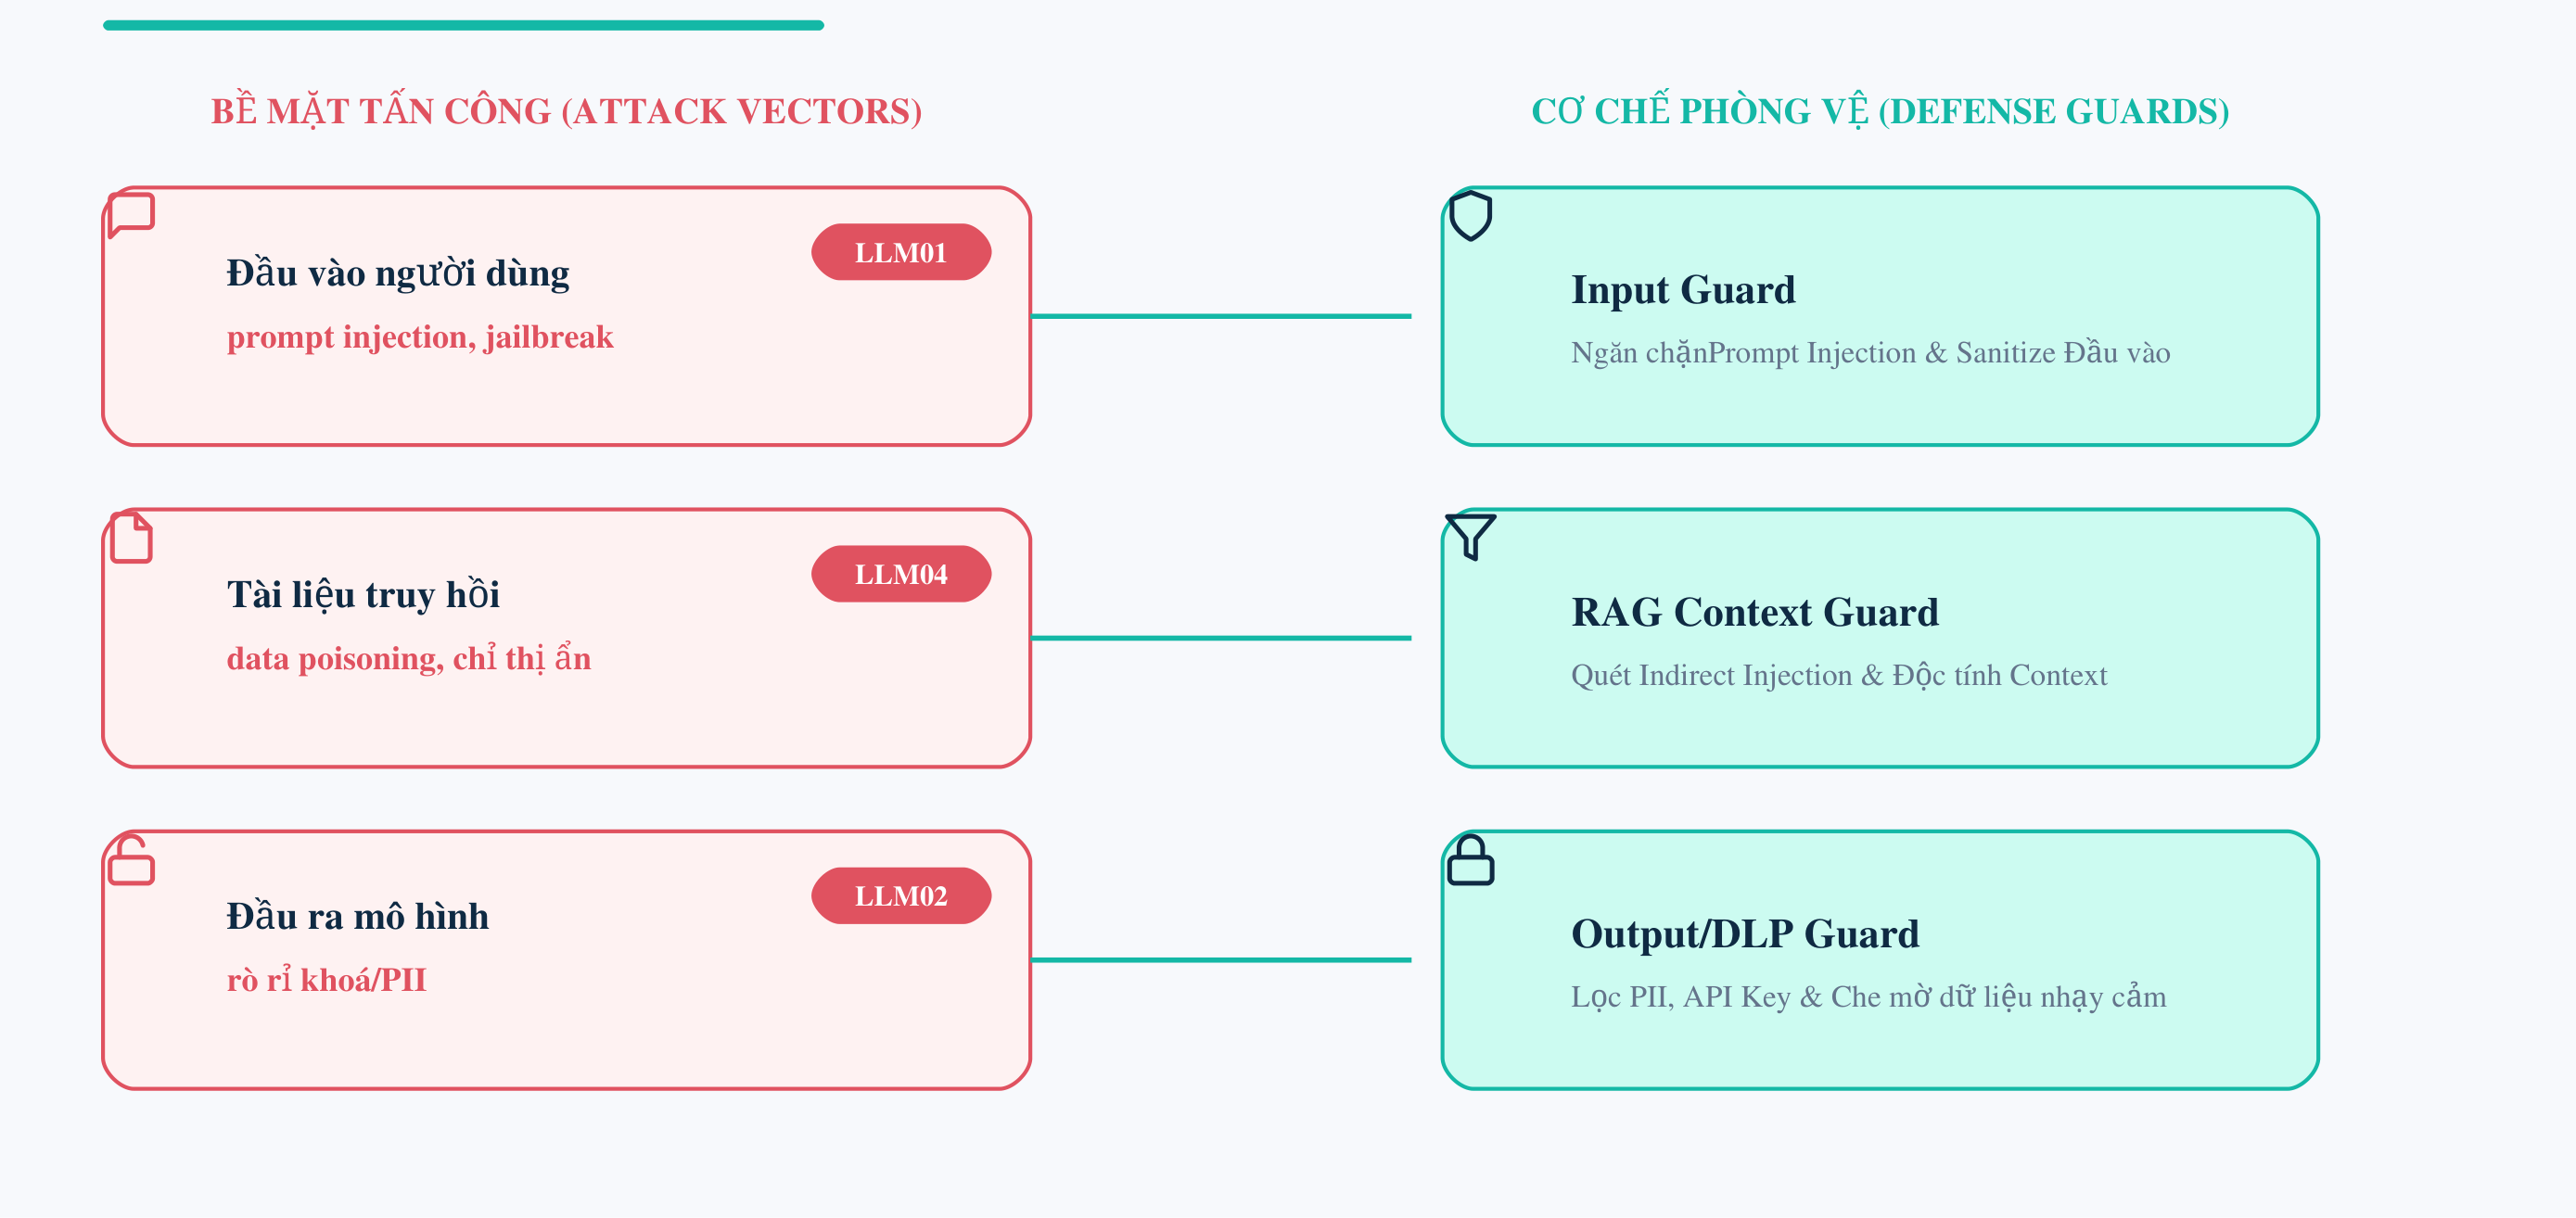
\includegraphics[width=0.75\linewidth]{figures/fig-threat-model.png}
\caption{Mô hình mối đe doạ: ba bề mặt tấn công và guard phòng vệ tương ứng}
\label{fig:threat-model}
\end{figure}

Hình~\ref{fig:threat-model} ánh xạ ba bề mặt tấn công của hệ thống RAG/LLM sang
lớp guard xử lý và mục tương ứng trong OWASP LLM Top 10: đầu vào người dùng
(prompt injection, jailbreak --- LLM01) do Input Guard xử lý; tài liệu truy hồi
(data poisoning, chỉ thị ẩn --- LLM04) do RAG Context Guard xử lý; và đầu ra mô
hình (rò rỉ khoá, PII --- LLM02) do Output/DLP Guard xử lý.

\section{Kết luận chương}

Chương này xác lập nền tảng: LLM/RAG mang lại năng lực mới nhưng mở rộng bề mặt tấn công. Kiểm soát cần đa lớp (đầu vào, ngữ cảnh, đầu ra) và phải đo được bằng kiểm thử có kiểm soát. Chương tiếp theo chuyển sang phân tích yêu cầu và thiết kế hệ thống của đề tài.

\chapter{Phân tích yêu cầu và thiết kế hệ thống}
\label{ch:phan-tich-thiet-ke}

\section{Khảo sát bài toán}

Bài toán đặt ra là xây dựng khung kiểm soát an toàn cho ứng dụng RAG/LLM quy mô lab. Hệ thống cần chặn hoặc xử lý prompt độc hại, giảm rò rỉ qua đầu ra, kiểm soát nguồn tài liệu và đảm bảo gói mã nguồn bàn giao không chứa artifact cấm. Yêu cầu học thuật nhấn mạnh tính tái lập, fail-closed và trung thực bằng chứng thay vì tối ưu hiệu năng production.

\section{Mục tiêu của hệ thống}

\begin{enumerate}
    \item Cung cấp cổng (gateway) trung gian xử lý yêu cầu RAG/chat với các lớp guard.
    \item Cho phép so sánh baseline (không guard) và có guard trên cùng bộ test tổng hợp.
    \item Đo và so sánh hiệu quả của tường trên bộ đánh giá bảo mật tổng hợp.
    \item Ghi nhật ký quyết định guard dạng content-free, không rò rỉ nội dung nhạy cảm thô.
\end{enumerate}

\section{Phạm vi chức năng}

\textbf{Trong phạm vi} gồm guard rule-based và Semantic Judge, RAG demo với BM25 kết hợp embedding, Mock Provider và mô hình cục bộ ollama, cùng bộ benchmark tấn công/lành tính tổng hợp. \textbf{Ngoài phạm vi} gồm fine-tune mô hình, SIEM, Kubernetes, multi-turn adversary thực chiến, và đánh giá trên LLM hay dữ liệu doanh nghiệp thật. Ranh giới này giúp giữ đề tài khả thi trong thời gian thực tập mà vẫn đủ để đo được hiệu quả tường.

\section{Yêu cầu chức năng}

\subsection{Kiểm tra dữ liệu đầu vào}
Hệ thống phải phát hiện các mẫu tấn công ở đầu vào như chèn chỉ dẫn (prompt
injection), jailbreak và yêu cầu trích xuất dữ liệu nhạy cảm. Với mỗi câu hỏi,
Input Guard trả về một quyết định thuộc tập Allow/Block/Sanitize/Log theo thiết
kế hành vi đã định nghĩa. Khi nhiều luật cùng khớp, quyết định nghiêm khắc nhất
được chọn để tránh bỏ lọt.

\subsection{Kiểm tra ngữ cảnh truy hồi}
Ngữ cảnh truy hồi từ kho tri thức có thể bị đầu độc bằng chỉ thị ẩn hoặc tài liệu
mạo danh thẩm quyền. RAG Context Guard phải quét các đoạn được truy hồi để phát
hiện những mẫu này trước khi đưa vào lời nhắc của mô hình. Với đoạn nghi ngờ, hệ
thống hỗ trợ làm sạch (sanitize) từng đoạn thay vì chặn toàn bộ câu trả lời, nhằm
giữ tính khả dụng.

\subsection{Kiểm tra dữ liệu đầu ra}
Trước khi trả phản hồi cho người dùng, Output Guard phải rà soát các mẫu nhạy cảm
như khoá API, token, PII và mã canary bị rò rỉ. Nếu phát hiện vi phạm rõ ràng, hệ
thống fail-closed (chặn hoặc che) thay vì trả nội dung ra ngoài. Đây là lớp phòng
thủ cuối cùng ở biên đầu ra, hoạt động độc lập với các guard đầu vào.

\subsection{Kiểm soát truy cập nguồn tài liệu}
Mỗi tài liệu trong kho mang thuộc tính vai trò, phòng ban và mức nhạy cảm. Hệ
thống phải áp kiểm soát truy cập theo vai trò (RBAC) ngay trước bước truy hồi, để
người dùng chỉ nhận được tài liệu trong phạm vi quyền của mình. Nhờ vậy, tài liệu
ngoài quyền không bao giờ lọt vào ngữ cảnh của mô hình, độc lập với các guard nội
dung.

\subsection{Ghi nhận và tổng hợp kết quả}
Mọi quyết định của guard phải được ghi nhật ký để phục vụ truy vết và đánh giá.
Bản ghi ở dạng JSON content-free, chỉ chứa mã lý do ổn định và nhãn quyết định,
không lưu nội dung nhạy cảm thô. Cách ghi này bảo đảm nhật ký có thể chia sẻ để
kiểm toán mà không trở thành một kênh rò rỉ dữ liệu mới.

\begin{table}[H]
\centering
\caption{Tóm tắt nhóm yêu cầu chức năng chính}
\label{tab:fr-summary}
\begin{tabular}{@{}p{0.18\linewidth}p{0.72\linewidth}@{}}
\toprule
\textbf{Mã nhóm} & \textbf{Mô tả} \\
\midrule
FR-IN  & Guard đầu vào kết hợp Tiền giải mã (Base64/ROT13/Leetspeak) và Semantic Judge \\
FR-CTX & Guard ngữ cảnh truy hồi (chỉ thị ẩn, poisoning, Provenance Guard) \\
FR-OUT & Guard đầu ra / DLP và làm sạch liên kết/hình ảnh thất thoát dữ liệu \\
FR-RAG & Pipeline truy hồi lai vectorized + kiểm soát truy cập RBAC trước truy hồi \\
FR-SQL & SQL Guard (\texttt{EXPLAIN} + Authorizer AST) và Indirect Data-Cell Result Guard \\
FR-AGT & Multi-Tool Company Agent với allowlist công cụ và hàng chờ phê duyệt cấp Leader \\
FR-LOG & Nhật ký kiểm toán/mã lý do ổn định, content-free \\
\bottomrule
\end{tabular}
\end{table}

\section{Yêu cầu phi chức năng}

\subsection{Tính an toàn}
Nguyên tắc an toàn cốt lõi là fail-closed: khi gặp đầu vào không hợp lệ, thiếu
thông tin tin cậy hoặc lỗi xử lý, hệ thống chọn quyết định an toàn (giữ lại câu
trả lời) thay vì mặc định cho qua. Điều này bảo đảm một lỗi ở một lớp không tự
động mở đường cho tấn công. Chi phí là đôi khi chặn nhầm, nhưng trong bối cảnh an
ninh, thận trọng được ưu tiên hơn tiện lợi.

\subsection{Tính tái lập}
Mọi kết quả đánh giá phải tái lập được để có thể kiểm chứng độc lập. Hệ thống
dùng hạt giống ngẫu nhiên cố định, Mock Provider tất định và băm SHA-256 cho các
artifact dữ liệu. Nhờ đó, cùng một commit mã nguồn và cùng bộ dữ liệu luôn cho ra
cùng số liệu.

\subsection{Tính xác định}
Với cấu hình rule-based, cùng một đầu vào luôn cho cùng một quyết định, không phụ
thuộc thời điểm chạy. Tính xác định này giúp giải thích được hành vi của tường và
loại bỏ nhiễu khi đo lường. Riêng cấu hình có Semantic Judge dùng mô hình ngôn
ngữ là phi tất định, được nêu rõ khi báo cáo số liệu.

\subsection{Khả năng kiểm tra}
Hệ thống đi kèm bộ kiểm thử tự động (pytest) bao phủ quyết định của từng guard và
pipeline RAG. Bộ chạy đánh giá bảo mật sinh artifact có thể tái lập, ghi kèm
provenance (commit, mô hình, cấu hình, băm dữ liệu). Nhờ đó, mỗi con số trong báo
cáo đều truy vết được về điều kiện đã tạo ra nó.

\subsection{Khả năng bảo trì}
Mã nguồn được tổ chức theo module cho từng guard và từng thành phần truy hồi,
giúp dễ đọc, dễ kiểm thử và dễ mở rộng. Các bí mật và cấu hình nhạy cảm không
được hard-code mà đọc từ biến môi trường. Cách tách bạch này giảm rủi ro khi thêm
luật mới hoặc thay đổi một lớp mà không ảnh hưởng lớp khác.

\section{Mô hình kiến trúc tổng thể}

Kiến trúc logic gồm ba lớp: (1)~lớp ứng dụng/gateway FastAPI; (2)~chuỗi guard phòng thủ nhiều lớp; (3)~cơ chế truy hồi lai kết hợp kiểm soát truy cập RBAC và mô hình ngôn ngữ (Mock hoặc cục bộ). Mọi lớp chia sẻ nguyên tắc fail-closed và ghi nhật ký content-free.

\begin{figure}[H]
\centering
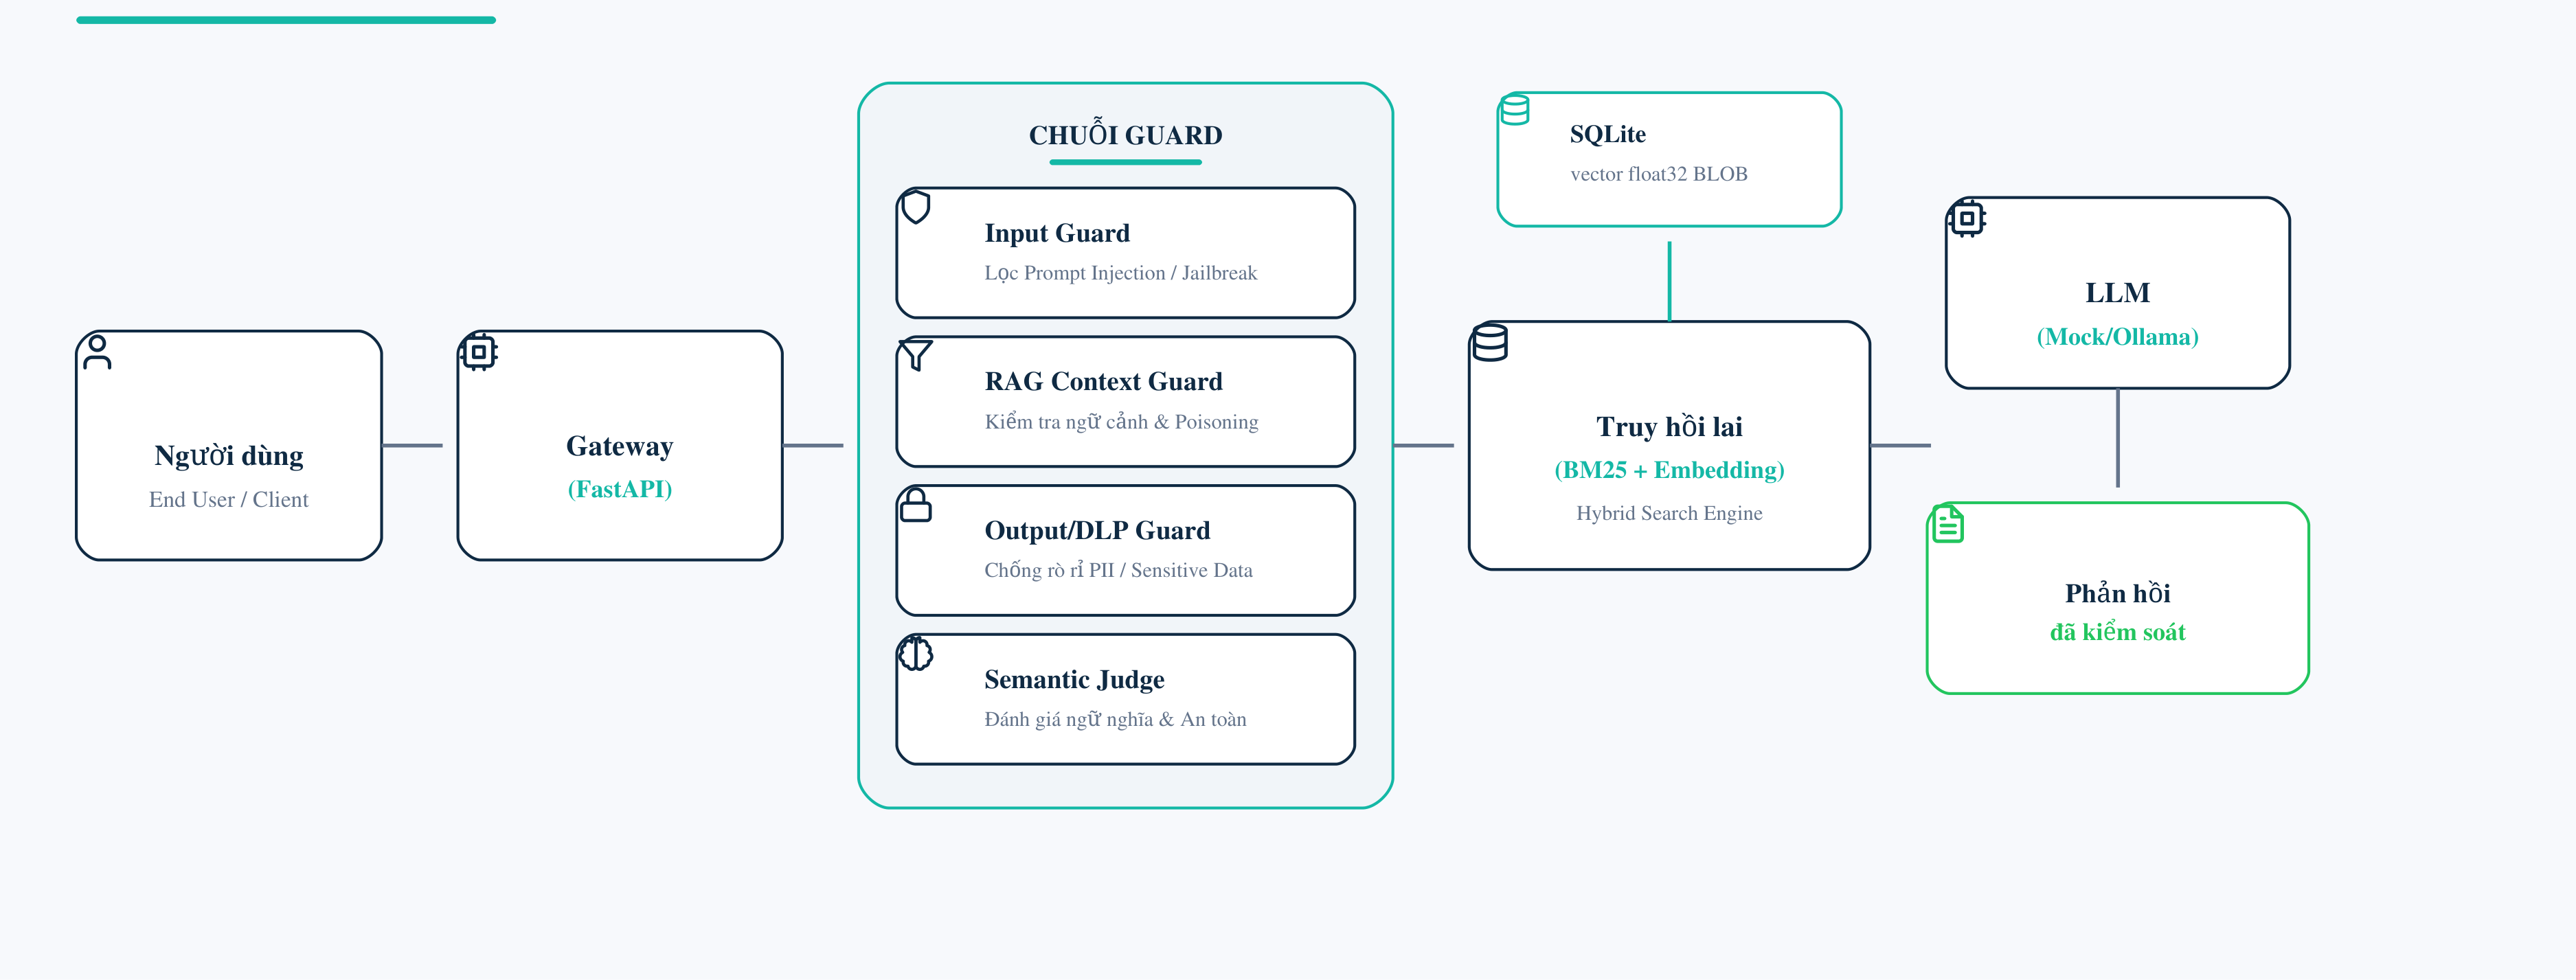
\includegraphics[width=0.78\linewidth]{figures/fig-kien-truc.png}
\caption{Kiến trúc tổng thể hệ thống Shield AI}
\label{fig:arch-logic}
\end{figure}

Hình~\ref{fig:arch-logic} mô tả đường đi của một yêu cầu từ trái sang phải: người
dùng gửi câu hỏi tới Gateway (FastAPI), qua chuỗi guard gồm Input Guard, RAG
Context Guard, Output/DLP Guard và Semantic Judge; bước truy hồi lai (BM25 kết
hợp embedding) đọc dữ liệu từ SQLite với vector \texttt{float32} lưu dạng BLOB,
trước khi câu hỏi tới mô hình ngôn ngữ và trả về phản hồi đã được kiểm soát.

\section{Kiến trúc phòng thủ nhiều lớp của Shield AI}

Hệ thống \textbf{Enterprise LLM Security Framework (Shield AI)} áp dụng nguyên
tắc \emph{phòng thủ theo chiều sâu} (defense-in-depth): mỗi yêu cầu đi qua một
chuỗi guard độc lập, mỗi guard chặn một lớp mối đe doạ khác nhau, và một guard
thất bại vẫn còn các lớp sau. Bốn lớp guard được hiện thực như sau.

\begin{table}[H]
\centering
\caption{Bốn lớp guard phòng thủ theo chiều sâu}
\label{tab:guard-layers}
\begin{tabularx}{\linewidth}{@{}p{0.24\linewidth}p{0.20\linewidth}X@{}}
\toprule
\textbf{Lớp guard} & \textbf{Cơ chế} & \textbf{Mối đe doạ xử lý} \\
\midrule
Input Guard & Luật regex/mẫu & Prompt injection trực tiếp, jailbreak, ghi đè chỉ thị hệ thống \\
RAG Context Guard & Luật trên ngữ cảnh truy hồi & Data poisoning, chỉ thị ẩn trong tài liệu, ngữ cảnh mạo danh thẩm quyền \\
Output Guard / DLP & Mẫu bí mật + DLP + canary & Rò rỉ khoá API, thông tin nhạy cảm, PII và mã canary seed từ kho trong phản hồi \\
Semantic Judge & LLM cục bộ phán đoán & Tấn công ngữ nghĩa (đóng vai, mạo danh cấp trên) mà luật không bắt được \\
\bottomrule
\end{tabularx}
\end{table}

Ba lớp đầu là \emph{tất định} (rule-based): cùng đầu vào luôn cho cùng quyết
định, dễ giải thích và không phụ thuộc mô hình. Lớp Semantic Judge là tuỳ chọn,
dùng một mô hình ngôn ngữ cục bộ để bắt các đòn tấn công dựa trên ngữ dụng xã
hội mà mẫu regex bỏ lọt --- đánh đổi lại là chi phí tính toán và rủi ro chặn
nhầm cao hơn (phân tích định lượng ở Chương~4).

\subsection{Cơ chế truy hồi tối ưu: Vectorized Hybrid Retrieval}

Trước khi qua các guard nội dung, ngữ cảnh được truy hồi bằng cơ chế lai
(hybrid) kết hợp: (1)~xếp hạng từ khoá BM25 trên SQLite FTS5, và (2)~xếp hạng
ngữ nghĩa bằng embedding cục bộ, hợp nhất bằng Reciprocal Rank Fusion.

Điểm ngữ nghĩa được tối ưu ở hai tầng. \textbf{Về lưu trữ}, vector embedding
được lưu dưới dạng khối nhị phân \texttt{float32} chuẩn hoá sẵn (BLOB) trong
SQLite thay vì chuỗi JSON; khi truy vấn chỉ cần đọc bộ nhớ (\texttt{memcpy})
thay vì phân tích lại hàng trăm số thực. \textbf{Về tính toán}, do vector đã
chuẩn hoá đơn vị nên độ tương đồng cosine chính là tích vô hướng, và toàn bộ
kho tài liệu được chấm điểm bằng \emph{một} phép nhân ma trận (\texttt{numpy})
thay vì vòng lặp Python trên từng tài liệu.

Về mặt độ phức tạp, cải tiến này thay chuỗi $N$ vòng lặp thông dịch (mỗi vòng
$D$ phép nhân--cộng) bằng một phép nhân ma trận được thư viện BLAS tối ưu, nên
độ trễ truy hồi trên kho 48 tài liệu doanh nghiệp chỉ mất trung vị $\text{p50} = 2{,}08\,\text{ms}$ ($\text{p95} = 5{,}27\,\text{ms}$, $\text{p99} = 6{,}66\,\text{ms}$ trên $1.275$ lượt đo thực nghiệm tại Chương~4).

\subsection{Kiến trúc bảo vệ Text-to-SQL và Multi-Tool Company Agent (P4 $\times$ P5)}

Để bảo vệ các ứng dụng trợ lý doanh nghiệp có kết nối cơ sở dữ liệu quan hệ và công cụ nghiệp vụ (mô phỏng qua doanh nghiệp nội thất Nhà Mộc Việt với 12 bảng SQL và 5 công cụ \texttt{search\_docs}, \texttt{query\_db}, \texttt{order\_status}, \texttt{create\_ticket}, \texttt{send\_email}), kiến trúc Shield AI được mở rộng với bốn chốt chặn chuyên biệt (Hình~\ref{fig:sql-agent-arch}):

\begin{enumerate}
    \item \textbf{SQLite \texttt{EXPLAIN} + Authorizer AST Guard (\texttt{app/sql\_agent/guard.py}):} Thay vì chỉ dựa vào biểu thức chính quy dễ bị vượt qua bởi bí danh (alias), bảng tạm (CTE), truy vấn con (subquery), \texttt{UNION} hoặc \texttt{SELECT *}, hệ thống biên dịch thử câu lệnh SQL bằng chính trình biên dịch của SQLite (\texttt{EXPLAIN}, không thực thi dữ liệu) trên một bản sao lược đồ rỗng trong bộ nhớ, đồng thời gắn hàm callback \texttt{sqlite3.set\_authorizer}. Trình biên dịch SQLite báo cáo chính xác mọi hành động \texttt{SQLITE\_READ(table, column)} và \texttt{SQLITE\_FUNCTION(func)}; nếu câu lệnh chạm vào bảng cấm (\texttt{internal\_secrets}, \texttt{sqlite\_master}, \texttt{pragma\_*}), vượt phạm vi bảng/cột được phép của cặp \emph{(phòng ban, vai trò)}, dùng hàm ngoài danh sách an toàn (\texttt{load\_extension}, \texttt{randomblob}, \texttt{char}) hoặc không phải câu lệnh chỉ đọc \texttt{SELECT/WITH}, SQL Guard chặn ngay lập tức và tự động bao bọc giới hạn \texttt{LIMIT $\le$ 50}.
    \item \textbf{Thực thi chỉ đọc cô lập (\texttt{app/sql\_agent/executor.py}):} Câu lệnh SQL hợp lệ được thực thi qua kết nối URI \texttt{mode=ro} kèm cờ \texttt{PRAGMA query\_only = ON}, gắn lại cùng bộ Authorizer AST và giới hạn thời gian/số dòng trả về.
    \item \textbf{Indirect Data-Cell Result Guard (\texttt{app/sql\_agent/result\_guard.py}):} Mọi ô văn bản tự do trả về từ cơ sở dữ liệu (như \texttt{orders.note}, \texttt{product\_reviews.comment}, \texttt{support\_tickets.content}) đều được xem là dữ liệu không đáng tin cậy và phải đi qua ba bộ lọc trước khi đưa vào lần gọi LLM thứ hai: (i)~chuẩn hoá bỏ ký tự ẩn zero-width, giải nhiễu gạch nối (\texttt{b-ỏ q-u-a}) và giải mã Base64 nhúng trong ô dữ liệu; (ii)~quét qua RAG Context Guard và bộ luật tiêm nhiễm SQL gián tiếp (\texttt{injection\_rules.py}: bắt thẻ giả mạo \texttt{[INST]}, lệnh đổi số tài khoản thanh toán, hình ảnh Markdown zero-click exfiltration, cú pháp gọi tool JSON); và (iii)~quét che mờ DLP. Ô vi phạm bị thay thế an toàn bằng nhãn \texttt{[nội dung bị giữ lại bởi Result Guard]}.
    \item \textbf{Kiểm soát công cụ theo phòng ban và Hàng chờ phê duyệt (\emph{Leader Approval Queue}):} Trong \texttt{app/company\_agent/}, mỗi phòng ban chỉ được phép gọi tập công cụ trong allowlist; mọi đầu ra của công cụ đều đi qua Result/RAG Guard; các hành động có tác động ghi hoặc gửi thông tin ra ngoài (như \texttt{send\_email}, \texttt{create\_ticket} nhạy cảm) bị chặn thực thi trực tiếp và đưa vào hàng chờ phê duyệt yêu cầu quyền \texttt{leader}, đồng thời giới hạn cứng tối đa 5 bước lặp công cụ.
\end{enumerate}

\begin{figure}[H]
\centering
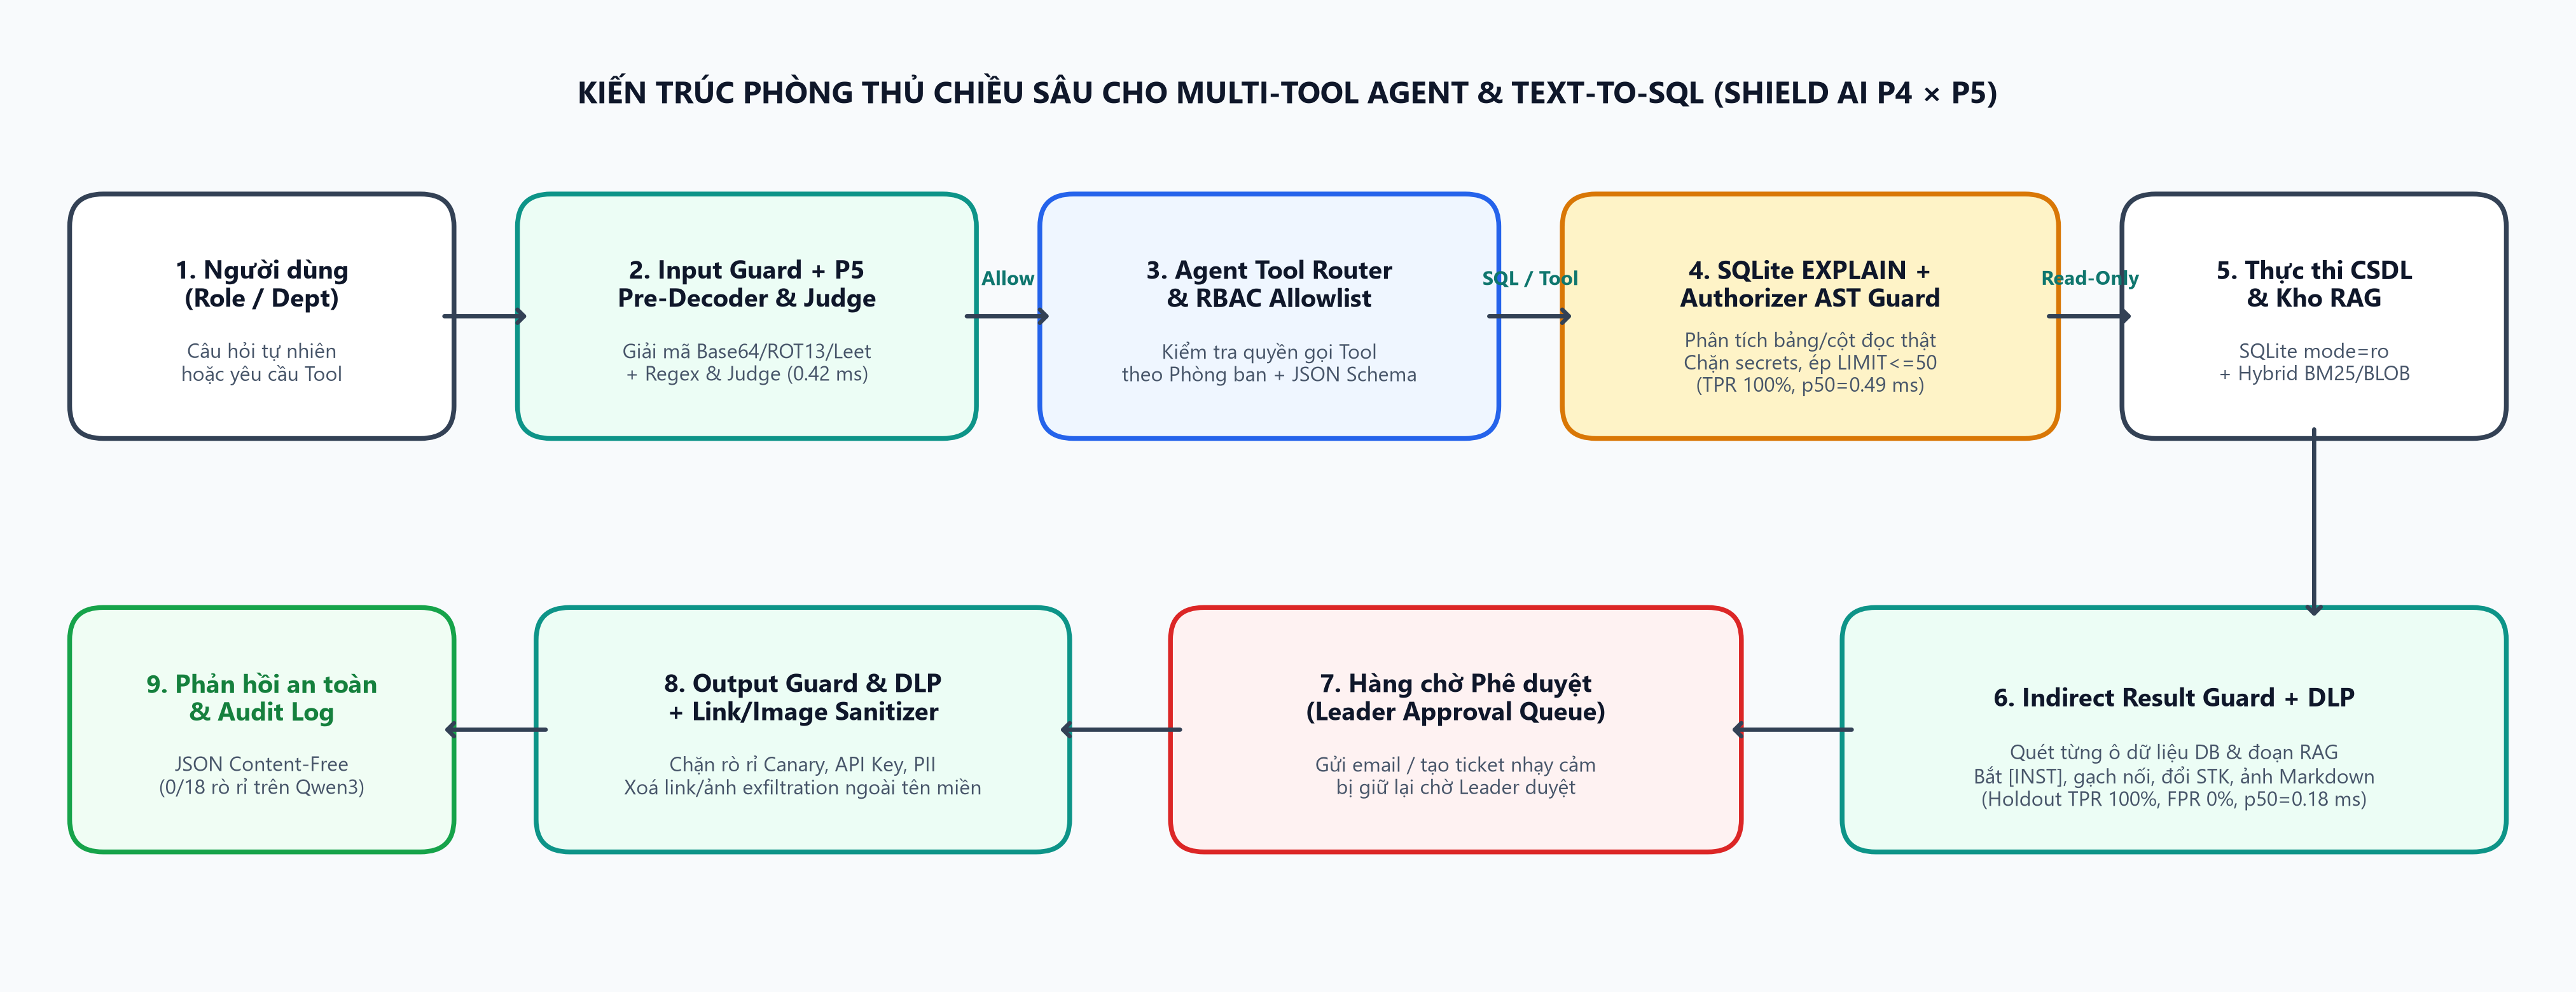
\includegraphics[width=0.95\linewidth]{figures/fig-sql-agent-architecture.png}
\caption{Kiến trúc phòng thủ chiều sâu cho Multi-Tool Agent và Text-to-SQL (Shield AI P4 $\times$ P5)}
\label{fig:sql-agent-arch}
\end{figure}

\subsection{Luồng A/B chuẩn hoá: có tường vs.\ không tường}

Để đánh giá tác dụng của tường lửa, hệ thống cung cấp hai luồng chat: \emph{có
tường} (Guarded, qua workspace store + ACL và toàn bộ chuỗi guard) và \emph{không
tường} (Unguarded, qua \texttt{unguarded\_store} và \emph{không} guard). Đây là
so sánh \emph{cấp hệ thống} (hai đường xử lý), không phải ``cùng một engine truy
hồi chỉ bật/tắt guard''. Để so sánh vẫn công bằng về dữ liệu, thí nghiệm gieo
\textbf{cùng một tài liệu KB (kèm canary) vào cả hai store}; do đó khác biệt
quan sát được quy về tác dụng của chuỗi guard trên cùng nội dung nguồn.

Cụ thể, luồng ``có tường'' đi qua chuỗi guard + workspace
store/ACL, còn luồng ``không tường'' đi qua \texttt{unguarded\_store} và bỏ qua
guard; cả hai được gieo \emph{cùng} tài liệu KB và cùng gọi một mô hình. Vì là so
sánh cấp hệ thống (hai luồng truy hồi riêng, không phải cùng một cơ chế truy hồi),
khác biệt quan sát được phản ánh tác dụng của chuỗi guard trên cùng nội dung nguồn.

\section{Luồng hoạt động của hệ thống}

\begin{figure}[H]
\centering
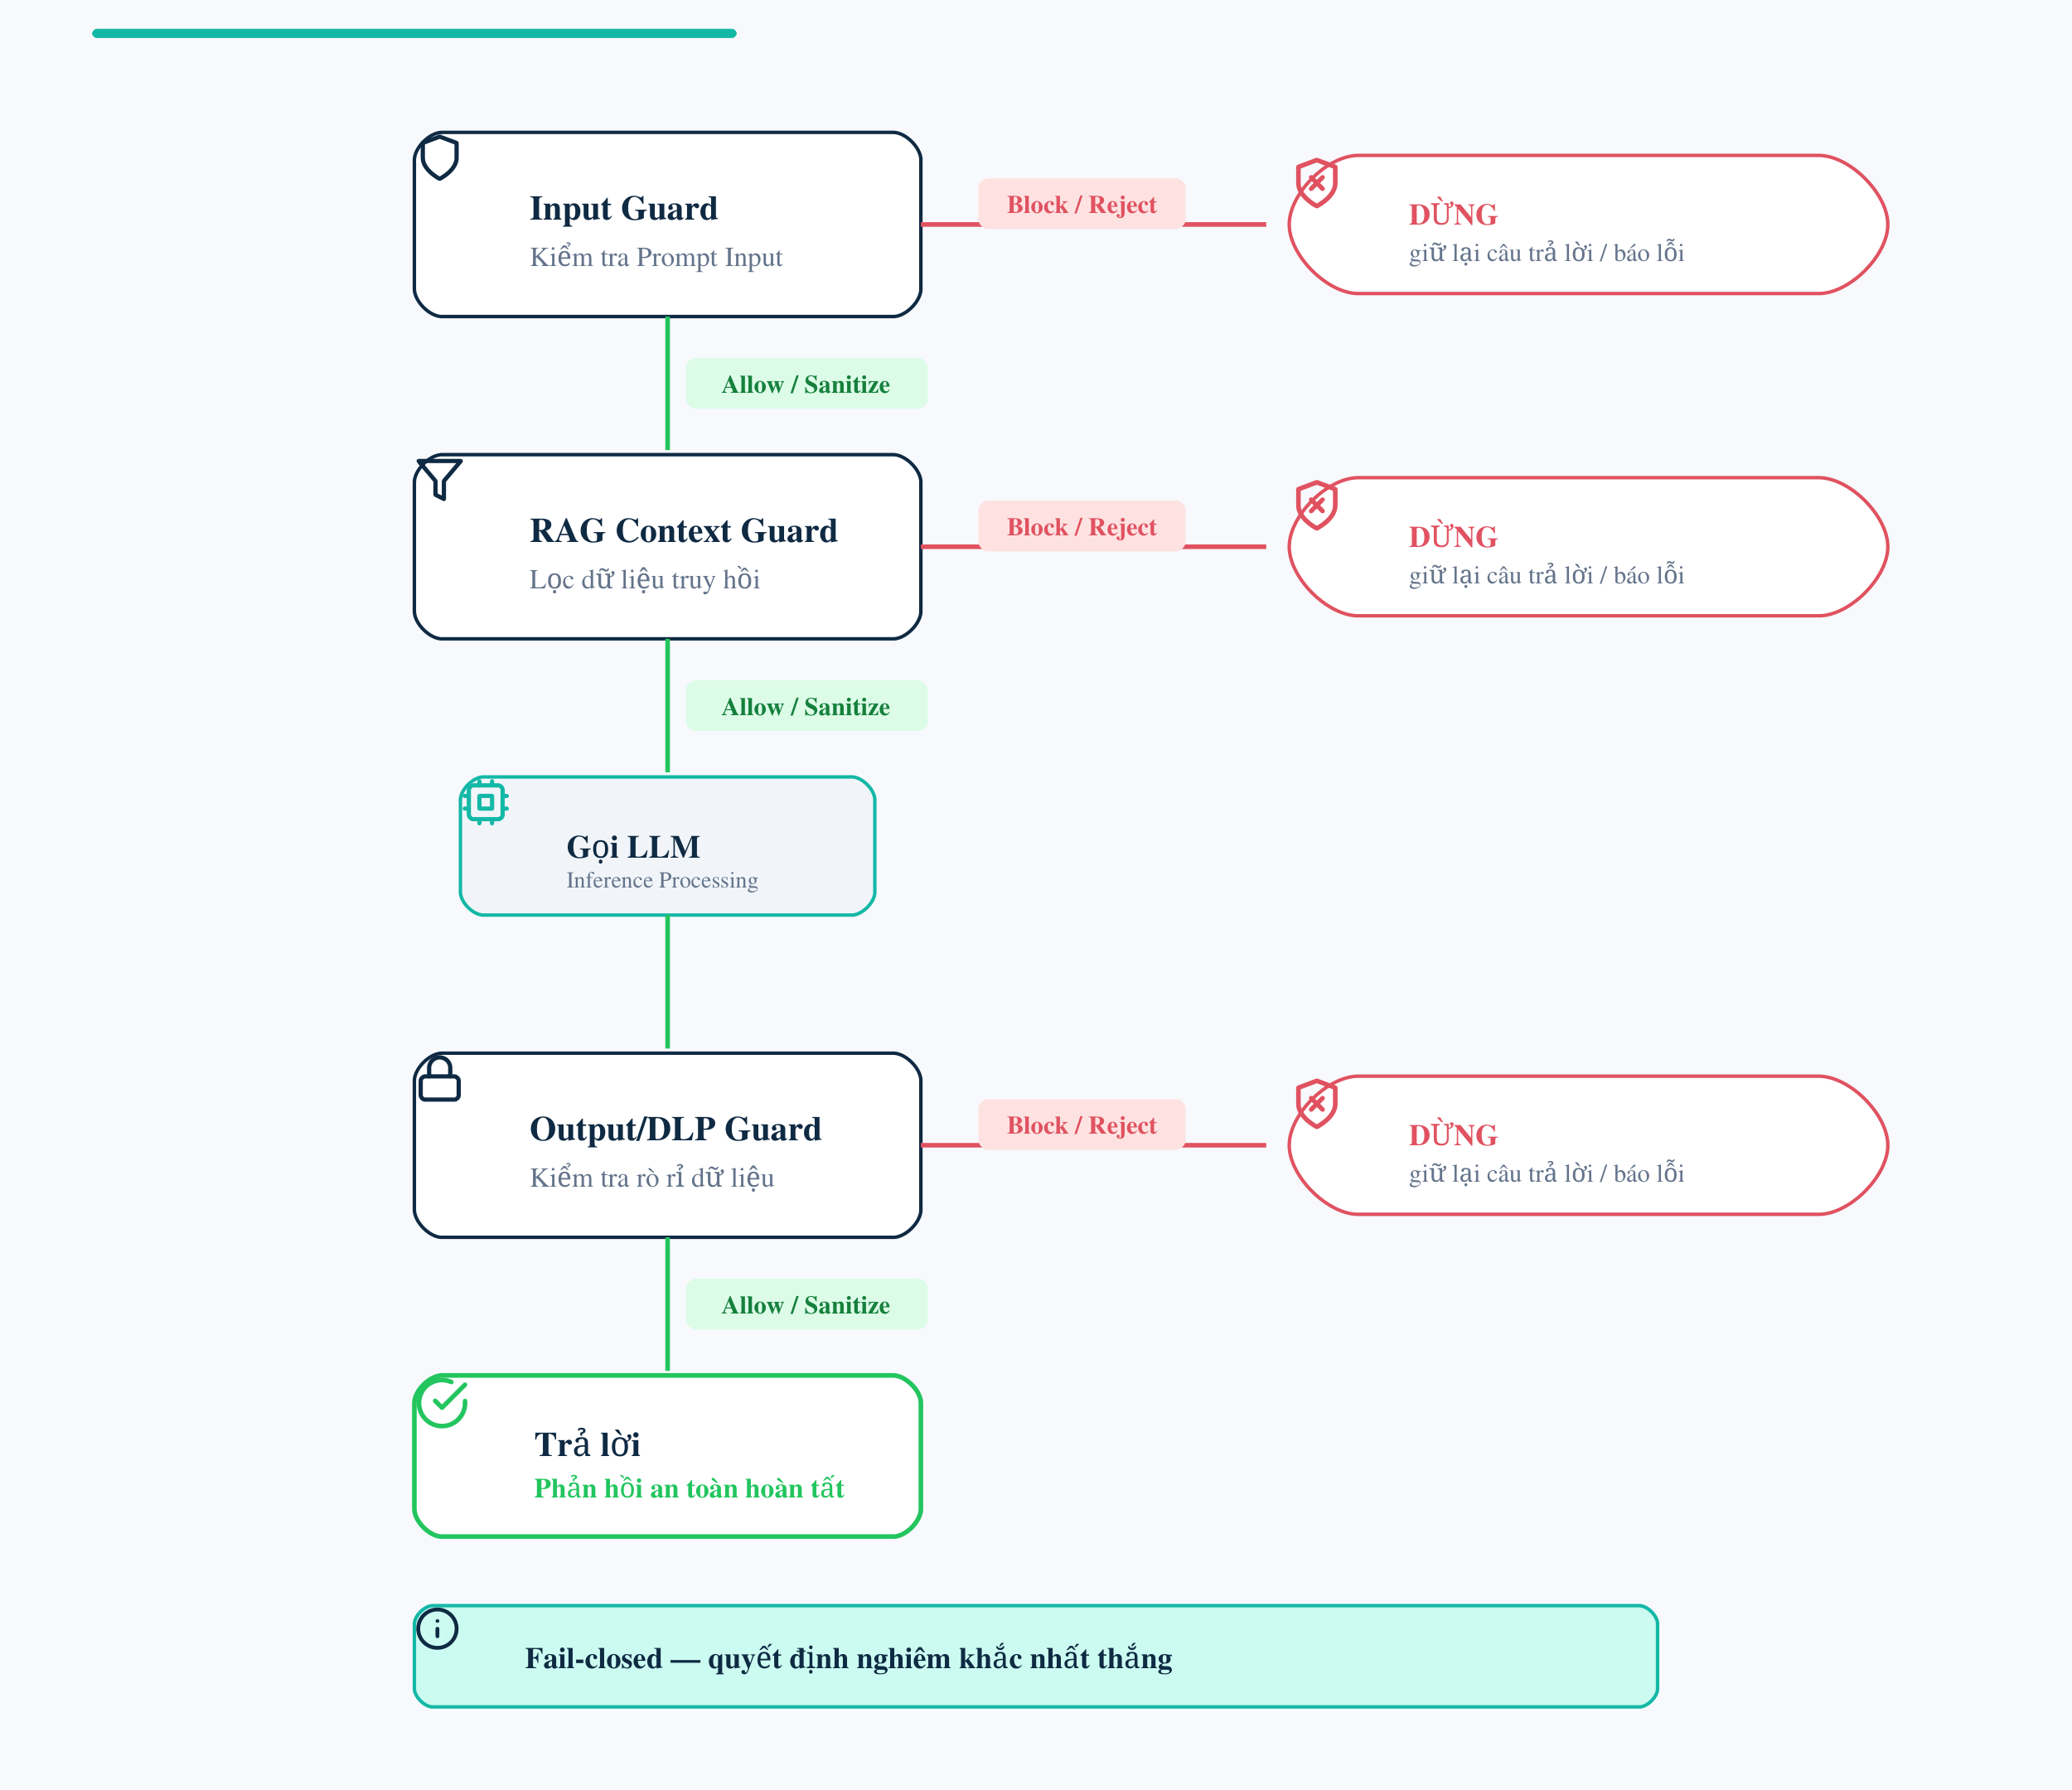
\includegraphics[width=0.6\linewidth]{figures/fig-phong-thu.png}
\caption{Chuỗi phòng thủ nhiều lớp và điểm quyết định fail-closed}
\label{fig:flow}
\end{figure}

Hình~\ref{fig:flow} thể hiện thứ tự xử lý qua các lớp guard. Tại mỗi lớp, quyết
định \emph{Block} hoặc \emph{Human-review} dừng luồng ngay và giữ lại câu trả
lời; quyết định \emph{Allow} hoặc \emph{Sanitize} cho phép đi tiếp sang lớp kế.
Nguyên tắc fail-closed bảo đảm quyết định nghiêm khắc nhất trong toàn chuỗi được
áp dụng.

\section{Thiết kế cơ chế xử lý lỗi}

Mọi lỗi trong đường xử lý được ánh xạ về quyết định an toàn: khi không chắc chắn
hoặc gặp lỗi phân tích, hệ thống fail-closed (giữ lại câu trả lời) thay vì mặc
định cho qua. Lỗi hệ thống bất ngờ được bọc ở biên công khai, không in nội dung
nhạy cảm hay traceback ra kênh công khai.

\section{Kết luận chương}

Yêu cầu và thiết kế nhấn mạnh phòng thủ nhiều lớp, fail-closed, kiểm soát truy
cập theo nguồn và tính tái lập. Chương~3 trình bày cách các thành phần được hiện
thực.

\chapter{Xây dựng và triển khai hệ thống}
\label{ch:xay-dung}

\section{Môi trường phát triển}

Hệ thống được phát triển trên Windows với Python 3.x trong môi trường ảo (\texttt{.venv}), quản lý mã bằng Git. Kiểm thử dùng \texttt{pytest}. Đường đánh giá lab không phụ thuộc dịch vụ LLM trực tuyến trả phí, nhằm giữ tính tái lập và kiểm soát chi phí.

\section{Công nghệ và công cụ sử dụng}

\begin{table}[!htbp]
\centering
\caption{Công nghệ, mô hình và công cụ kiểm thử độc lập sử dụng trong đồ án}
\label{tab:tech}
\begin{tabular}{@{}L{0.28\linewidth}L{0.62\linewidth}@{}}
\toprule
\textbf{Thành phần} & \textbf{Lựa chọn} \\
\midrule
Ngôn ngữ \& Môi trường & Python 3.13, Windows 11, NVIDIA GeForce RTX~4050 (6\,GB VRAM) \\
API Gateway & FastAPI / Starlette / Uvicorn \\
Lưu trữ \& Truy hồi lai & SQLite FTS5 (BM25) kết hợp embedding vector \texttt{float32} BLOB + nhân ma trận \texttt{numpy} \\
Kiểm soát truy cập & Pre-retrieval RBAC (tài liệu RAG) + SQLite \texttt{EXPLAIN} \& Authorizer AST (bảng/cột SQL) \\
Mô hình LLM \& Judge cục bộ & Ollama 0.40.11: \texttt{gemma4:e2b-\allowbreak it-\allowbreak q4\_\allowbreak K\_\allowbreak M} (Semantic Judge 2B tối ưu \texttt{think=False}), \texttt{gemma4:e4b-\allowbreak it-\allowbreak qat}, \texttt{qwen3:4b-\allowbreak instruct} (Multi-Tool Agent) và \texttt{claude-\allowbreak sonnet-\allowbreak 5-\allowbreak 5} adapter \\
Giải pháp đối sánh (Baselines) & Meta \texttt{llama-\allowbreak guard3:1b} (Ollama), NVIDIA \texttt{NeMo Guardrails} (\texttt{self\_\allowbreak check\_\allowbreak input} rail) \\
Công cụ \& Benchmark độc lập & NVIDIA \texttt{garak v0.\allowbreak 17.\allowbreak 1} ($2.048$ REST probes), \texttt{PyRIT} Converter \& Adaptive Multi-Turn, HuggingFace \texttt{deepset/\allowbreak prompt-\allowbreak injections} ($662$ mẫu) \\
Kiểm thử tự động & \texttt{pytest} ($469+$ unit \& integration tests trên nhánh hợp nhất) \\
\bottomrule
\end{tabular}
\end{table}

\section{Tổ chức mã nguồn}

Mã nguồn được nhóm theo chức năng để dễ đọc, dễ kiểm thử và tách bạch trách
nhiệm giữa các thành phần. Cụ thể: \texttt{app/} chứa gateway, các guard và
pipeline RAG; \texttt{scripts/} chứa mã sinh dữ liệu và chạy đánh giá;
\texttt{tests/} chứa bộ kiểm thử pytest; \texttt{datasets/} chứa bộ dữ liệu tấn
công và lành tính tổng hợp; \texttt{docs/} lưu tài liệu thiết kế và các quyết
định kỹ thuật. Cách phân tách này giúp thay đổi một lớp guard hoặc một thành phần
truy hồi mà ít ảnh hưởng tới phần còn lại của hệ thống.

\section{Xây dựng chuỗi guard phòng thủ}

Chuỗi guard được hiện thực thành các module độc lập trong \texttt{app/\allowbreak guards/},
mỗi module trả về quyết định trong tập \{Allow, Block, Sanitize, Human-review,
Log\} theo thứ tự mức độ nghiêm trọng cố định (\emph{fail-closed}: quyết định
nghiêm khắc nhất thắng).

\begin{itemize}
    \item \textbf{Input Guard kết hợp Tầng tiền giải mã (\emph{Payload De-obfuscation Pre-decoder}):} Trước khi đối chiếu bộ luật regex, hàm \texttt{\_\allowbreak expand\_\allowbreak deobfuscated\_\allowbreak views()} trong \texttt{app/\allowbreak guards/\allowbreak input\_\allowbreak guard.\allowbreak py} thực hiện chuẩn hoá Unicode NFKC, loại bỏ ký tự ẩn zero-width (\texttt{U+200B..\allowbreak U+FEFF}), gấp đồng hình Cyrillic về Latin, giải nhiễu Leetspeak (\texttt{4->a, 3->e, 1->i, 0->o, 5->s, 7->t}), tự động phát hiện và giải mã các khối Base64 sang UTF-8, cũng như dịch ngược ROT13 khi có tín hiệu mã hoá. Nhờ đó, bộ luật cấu trúc đa ngôn ngữ (Việt/Anh/Đức/Tây Ban Nha) nhìn thấy trực tiếp cả lớp vỏ bọc lẫn mệnh lệnh độc hại ẩn bên trong.
    \item \textbf{RAG Context Guard \& Provenance Guard:} Kiểm tra nguồn gốc tài liệu do máy chủ gán (\texttt{source\_\allowbreak policy.\allowbreak py}) và đối chiếu luật trên từng đoạn ngữ cảnh truy hồi nhằm phát hiện chỉ thị ẩn trong bình luận HTML, giả mạo thẻ hệ thống và mẫu đầu độc kho tri thức; hỗ trợ làm sạch (sanitize) từng đoạn và fail-closed khi bằng chứng tốt nhất bị vô hiệu hoá.
    \item \textbf{SQLite Authorizer AST Guard \& Indirect Result Guard:} Trong \texttt{app/\allowbreak sql\_\allowbreak agent/}, câu lệnh SQL do mô hình sinh ra được kiểm tra bằng \texttt{EXPLAIN} + \texttt{set\_\allowbreak authorizer} trên lược đồ rỗng để cưỡng chế phân quyền tới từng bảng/cột và ép \texttt{LIMIT $\le$ 50}; kết quả trả về từ CSDL tiếp tục được quét từng ô qua \texttt{result\_\allowbreak guard.\allowbreak py} (giải nhiễu gạch nối \texttt{b-ỏ q-u-a}, bắt thẻ \texttt{[INST]}, chặn đổi số tài khoản và che mờ DLP) trước khi đưa vào lần gọi mô hình thứ hai.
    \item \textbf{Output Guard / DLP:} Rà mẫu bí mật (khoá API, JWT, mật khẩu), thông tin định danh cá nhân (PII), liên kết/hình ảnh Markdown thất thoát dữ liệu ra tên miền lạ và mã canary seed từ kho trên phản hồi trước khi trả về người dùng.
    \item \textbf{Semantic Judge cục bộ tối ưu độ trễ (\texttt{gemma4:e2b-\allowbreak it-\allowbreak q4\_\allowbreak K\_\allowbreak M}):} Trong \texttt{app/\allowbreak guards/\allowbreak semantic\_\allowbreak guard.\allowbreak py}, yêu cầu đi qua bộ lọc nhanh (\emph{fast heuristic pre-screen}, $< 0{,}2\,\text{ms}$) và cơ chế \emph{benign short-circuit}; chỉ các truy vấn nằm ở vùng nghi ngờ mới gọi tới mô hình Judge 2B qua Ollama với tham số \texttt{"think": False} và \texttt{num\_\allowbreak predict: 8}, giữ độ trễ mỗi lần gọi Judge ở mức trung vị $\text{p50} = 99{,}79\,\text{ms}$ thay vì hàng nghìn mili-giây như các cấu hình sinh chuỗi suy nghĩ ngầm.
\end{itemize}

\section{Xây dựng cơ chế truy hồi vectorized}

Cơ chế truy hồi lai kết hợp BM25 (SQLite FTS5) với xếp hạng ngữ nghĩa. Để giảm
độ trễ khi kho tài liệu lớn, vector embedding được chuẩn hoá đơn vị và lưu dưới
dạng khối \texttt{float32} (BLOB) trong SQLite; khi truy vấn, toàn bộ ma trận
vector được đọc trực tiếp và chấm điểm bằng \emph{một} phép nhân ma trận
\texttt{numpy} (tích vô hướng chính là cosine do vector đã chuẩn hoá), thay cho
vòng lặp Python và phân tích JSON trên từng tài liệu. Hai danh sách xếp hạng
được hợp nhất bằng Reciprocal Rank Fusion.

Kiểm soát truy cập (RBAC) được áp \emph{trước} bước truy hồi: mỗi tài liệu mang
vai trò/phòng ban và mức nhạy cảm; người dùng chỉ truy hồi được tài liệu trong
phạm vi quyền, độc lập với các guard nội dung.

\begin{figure}[!htbp]
\centering
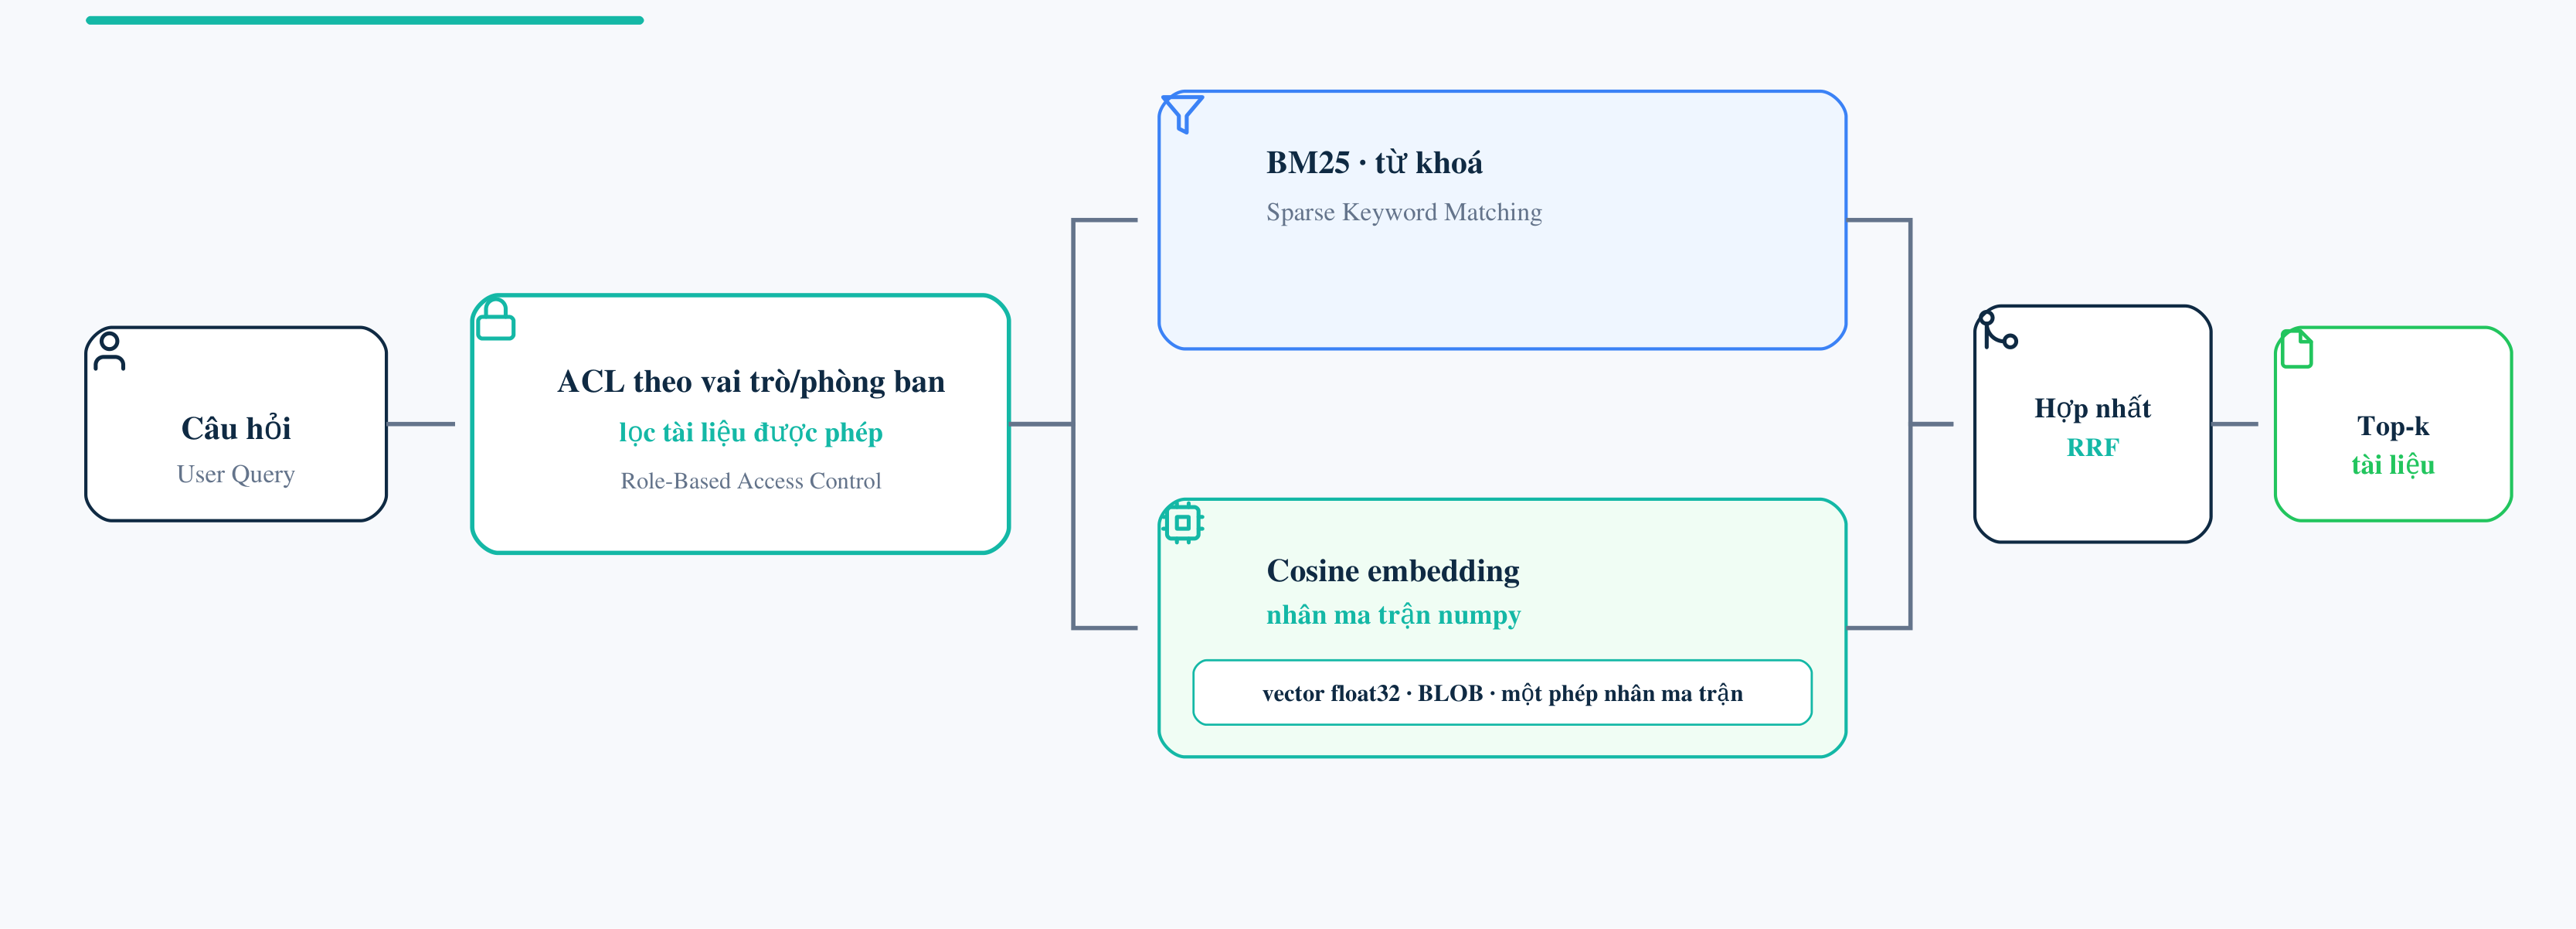
\includegraphics[width=0.78\linewidth]{figures/fig-rag-rbac.png}
\caption{Cơ chế truy hồi lai (BM25 + embedding) kết hợp kiểm soát truy cập RBAC}
\label{fig:rag-rbac}
\end{figure}

Hình~\ref{fig:rag-rbac} minh hoạ luồng: câu hỏi trước hết qua bộ lọc ACL theo
vai trò/phòng ban, sau đó được chấm điểm song song bằng BM25 (từ khoá) và cosine
embedding (nhân ma trận trên vector \texttt{float32}), rồi hai danh sách được hợp
nhất bằng Reciprocal Rank Fusion để chọn ra tài liệu liên quan nhất.

\section{Tích hợp kiểm thử tự động}

Bộ kiểm thử tự động (pytest) bao phủ quyết định của từng guard, pipeline RAG
end-to-end, kiểm soát truy cập RBAC và các kịch bản hồi quy canary/DLP. Mục tiêu
là phát hiện sớm hồi quy khi chỉnh luật hoặc runner, đồng thời giữ bằng chứng
có thể chạy lại trên cùng môi trường lab. Bộ chạy đánh giá ghi kèm provenance
tối thiểu (commit, mô hình, cấu hình, băm dữ liệu) cho các lần chạy mới để truy
vết. Chi tiết kết quả trình bày ở Chương~4.

\section{Kết luận chương}

Chương này trình bày hiện thực chuỗi guard phòng thủ nhiều lớp và cơ chế truy hồi
vectorized kết hợp kiểm soát truy cập RBAC, theo nguyên tắc fail-closed,
content-free và tái lập. Chương~4 trình bày phương pháp và kết quả kiểm thử.

\chapter{Kiểm thử và đánh giá kết quả}
\label{ch:kiem-thu}

\section{Mục tiêu kiểm thử}

\begin{enumerate}
    \item Xác nhận chuỗi guard đa lớp, pipeline RAG có RBAC, SQLite Authorizer AST Guard và Multi-Tool Company Agent hoạt động chính xác qua bộ kiểm thử tự động ($469+$ unit \& integration tests).
    \item Đánh giá hiệu quả phát hiện trên bộ dữ liệu tổng hợp nội bộ ($425$ case) và \textbf{kiểm chứng độc lập} trên bộ benchmark công khai ngoài phân phối \texttt{deepset/\allowbreak prompt-\allowbreak injections} ($662$ mẫu đa ngôn ngữ) trước và sau khi nâng cấp kiến trúc P5.
    \item Thực hiện \textbf{đối sánh định lượng} công bằng giữa \textbf{Shield AI} (Rule-Only và Rule + Semantic Judge \texttt{gemma4:e2b}) với hai giải pháp chuẩn quốc tế là \textbf{Meta Llama Guard~3 1B} (\texttt{llama-\allowbreak guard3:1b}) và \textbf{NVIDIA NeMo Guardrails} (\texttt{self\_\allowbreak check\_\allowbreak input}) trên cùng tập dữ liệu và cùng phần cứng.
    \item Đo đạc đầy đủ phân vị độ trễ \textbf{\texttt{p50 / p95 / p99}} cho từng tầng xử lý (Input Guard, Semantic Pre-screen, Semantic Judge LLM, RAG Context Guard, Output/DLP Guard, Retrieval, SQL Guard, Indirect Result Guard) khi bật và tắt Semantic Judge.
    \item Bắn trực tiếp công cụ red-team độc lập \textbf{\texttt{NVIDIA garak v0.\allowbreak 17.\allowbreak 1}} ($2.048$ probe qua HTTP REST) và bộ biến đổi/tấn công thích nghi đa lượt \textbf{\texttt{PyRIT}} vào các endpoint sống (\texttt{/\allowbreak v1/\allowbreak rag/\allowbreak query}, \texttt{/\allowbreak v1/\allowbreak gateway/\allowbreak chat}, \texttt{/v1/conversations/\{id\}/messages}).
\end{enumerate}

\section{Phương pháp kiểm thử}

Nhóm kết hợp: (i)~kiểm thử đơn vị/tích hợp bằng pytest cho các guard và pipeline RAG; (ii)~đánh giá hiệu quả bảo mật trên bộ tấn công/lành tính tổng hợp với ba cấu hình guard; (iii)~thí nghiệm tối ưu lớp luật, đo trước/sau trên cùng bộ dữ liệu.

\section{Môi trường kiểm thử}

Toàn bộ kiểm thử chạy trong môi trường ảo Python (\texttt{.venv}) để cô lập phụ
thuộc. Bộ pytest dùng thư mục tạm ngoài repo khi cần, tránh làm bẩn cây mã nguồn.
Đường đánh giá chính không gọi mạng (Mock Provider tất định); riêng cấu hình
Semantic Judge dùng mô hình cục bộ chạy qua ollama, không phụ thuộc dịch vụ trực
tuyến.

\section{Các nhóm kiểm thử}

\subsection{Kiểm thử chức năng}
Nhóm kiểm thử chức năng xác nhận từng thành phần cho quyết định đúng trên các ca
đại diện. Phạm vi bao phủ quyết định của từng guard (đầu vào, ngữ cảnh, đầu ra),
pipeline RAG và cơ chế kiểm soát truy cập theo vai trò (RBAC). Mỗi ca kiểm thử cố
định đầu vào và kỳ vọng đầu ra, nhờ đó lỗi hồi quy được phát hiện ngay khi mã
nguồn thay đổi.

\subsection{Kiểm thử lỗi và fail-closed}
Nhóm kiểm thử này xác nhận hệ thống xử lý đúng các tình huống vi phạm và lỗi. Cụ
thể, nó kiểm tra nguyên tắc ``quyết định nghiêm khắc nhất thắng'' khi nhiều guard
cùng phát hiện vấn đề, và hành vi fail-closed khi có vi phạm rõ ràng. Mục tiêu là
bảo đảm một lỗi cục bộ không khiến hệ thống mặc định cho câu trả lời đi qua.

\section{Kịch bản kiểm thử chính}

\begin{itemize}
    \item Baseline (always-allow) so với có guard trên bộ đánh giá bảo mật tổng hợp.
    \item Ba cấu hình guard (rule-based, Semantic Judge \texttt{qwen3:4b}, đối chiếu \texttt{hermes3:8b}) trên cùng bộ 425 case.
    \item Thí nghiệm tối ưu lớp luật: đo TPR/FPR trước và sau trên cùng dữ liệu.
\end{itemize}

\section{Kết quả kiểm thử tự động}

\begin{table}[!htbp]
\centering
\caption{Tổng hợp kết quả kiểm thử tự động tích hợp (Nhánh \texttt{feat-\allowbreak p5-\allowbreak integrated-\allowbreak thesis})}
\label{tab:test-summary}
\begin{tabular}{@{}L{0.58\linewidth}L{0.34\linewidth}@{}}
\toprule
\textbf{Nhóm kiểm thử (\texttt{pytest})} & \textbf{Kết quả} \\
\midrule
Input Guard, RAG Context Guard, Output/DLP Guard \& Semantic Judge & $151$ passed, $0$ failed \\
Pipeline RAG, Provenance Guard, Canonical I/O \& Ollama Provider & $180$ passed, $0$ failed \\
Text-to-SQL Guard (Authorizer AST), Result Guard \& Company Agent (Nhà Mộc Việt) & $138$ passed, $0$ failed \\
\textbf{Tổng bộ kiểm thử tích hợp P2 + P3 + P4 + P5} & \textbf{469 passed, 0 failed ($3{,}61\,\text{s}$)} \\
\textbf{Full repository regression suite (\texttt{verify\_\allowbreak phase.\allowbreak ps1})} & \textbf{1708 passed, 0 failed, 4 skipped} \\
\bottomrule
\end{tabular}
\end{table}

Các số liệu trên là kết quả kiểm thử tự động của hệ thống lab, \textbf{không} phải chỉ số hiệu quả bảo mật trên môi trường thật.

\section{Đánh giá hiệu quả bảo mật trên bộ tấn công tổng hợp}
\label{sec:sec-eval}

Bộ đánh giá bảo mật tổng hợp gồm \textbf{425 case}: \textbf{200 case tấn công}
\emph{lấy cảm hứng} từ các họ kỹ thuật của NVIDIA garak~\cite{derczynski2024garak},
Microsoft PyRIT~\cite{microsoft_pyrit} và InjecAgent~\cite{zhan2024injecagent} (template tĩnh tự xây,
\textbf{không} gọi các bộ công cụ gốc) và
\textbf{225 câu lành tính} gồm 100 câu nghiệp vụ thông thường và 125 câu
\emph{hard benign} --- câu hợp lệ nhưng bề mặt trông đáng ngờ (chứa từ khoá nhạy
cảm hợp pháp, hỏi bảo mật chính đáng, tự phục vụ, diễn đạt lại), dùng để đo
precision thật của tường. Toàn bộ payload là dữ liệu tổng hợp, sinh xác định.
Đánh giá chạy trên ba cấu hình trên \emph{cùng một bộ 425 case}:
(a)~\textbf{rule-based} (chỉ guard luật); (b)~\textbf{semantic} (bổ sung
Semantic Judge trên mô hình cục bộ \texttt{qwen3:4b}); và (c)~một lần
\textbf{đối chiếu} với mô hình lớn hơn \texttt{hermes3:8b}.

Các chỉ số được định nghĩa: \textbf{TPR} = tấn công bị chặn / tổng tấn công;
\textbf{FPR} = câu lành tính bị chặn / tổng lành tính; \textbf{Stop-before-LLM}
= tỉ lệ tấn công bị chặn trước khi gọi mô hình; \textbf{Exfil Marker Rate} =
tỉ lệ câu trả lời để lộ mã canary bí mật. Ở giai đoạn cơ sở trên tập 425 case này, các chỉ số phát hiện được đo độc lập với thời gian phản hồi; phép đo phân vị độ trễ \texttt{p50/\allowbreak p95/\allowbreak p99} của từng tầng được trình bày chuyên sâu tại Mục~\ref{sec:latency-eval}.

\textbf{Lựa chọn và ý nghĩa chỉ số.} Với một tường guard, hai chỉ số TPR và FPR
không cùng vai trò. \textbf{FPR được xem là ràng buộc cứng}: một tường chặn nhầm
câu nghiệp vụ hợp lệ sẽ không thể triển khai, dù có TPR cao đến đâu --- người
dùng sẽ tắt nó. Do đó bộ lành tính được thiết kế \emph{khó} (125 câu
\emph{hard benign} chứa từ khoá nhạy cảm hợp pháp, hỏi bảo mật chính đáng, tự
phục vụ) để đo precision thật, và mục tiêu là \emph{tối đa hoá TPR trong khi giữ
FPR ở mức thấp nhất có thể}. \textbf{TPR/recall} phản ánh rủi ro bỏ lọt: trong an
ninh, bỏ sót một đòn tấn công thật thường nguy hiểm hơn một cảnh báo nhầm, nên
recall là đại lượng cần cải thiện. \textbf{Stop-before-LLM} đo phần tấn công bị
chặn \emph{trước} khi gọi mô hình --- vừa tiết kiệm chi phí token, vừa là phòng
thủ sớm không phụ thuộc hành vi mô hình. \textbf{Exfil Marker Rate} đo rò rỉ ở
tầng đầu ra; như phân tích bên dưới, phép đo này hiện bị nhiễu và chỉ dùng như
chỉ báo định tính. Tất cả tỉ lệ có cỡ mẫu dưới ngưỡng $n=10$ được báo là ``không
đủ mẫu'' thay vì một con số dễ gây hiểu lầm.

\textbf{Tối ưu lớp luật.} Lần đánh giá đầu cho thấy lớp luật bỏ lọt hoàn toàn họ
PyRIT (đóng vai/mạo danh thẩm quyền, $0\%$). Chúng tôi bổ sung một nhóm luật
nhắm \emph{hai bất biến từ vựng} của đòn mạo danh (cụm từ đặc trưng, không phải đặc trưng ngữ nghĩa) --- chỉ thị vượt quyền (ghi đè chính
sách/ACL, ``không được từ chối cấp trên'') và yêu cầu trích xuất hàng loạt dữ
liệu nhạy cảm --- thay vì khớp đúng câu chữ của từng case. Trên cùng bộ 425
case, thay đổi này nâng TPR của lớp luật từ $48{,}5\%$ lên $77{,}0\%$ mà
\textbf{giữ nguyên FPR $0\%$ trên bộ 225 câu lành tính tổng hợp}. Bước tối ưu thứ
hai --- \textbf{chuẩn hoá đầu vào} trước khi đối chiếu luật (NFKC, loại ký tự ẩn
zero-width, gấp các đồng hình Cyrillic về Latin) --- vô hiệu hoá kỹ thuật ``làm
rối Unicode'' của garak, nâng tiếp TPR lên $\mathbf{81{,}5\%}$ (garak
$75{,}2\%\to83{,}8\%$) vẫn ở FPR $0\%$ (Bảng~\ref{tab:v3-optim}). Đây là bước
giải nhiễu \emph{tổng quát}, không tinh chỉnh theo case cụ thể. \textbf{Bước tối
ưu thứ ba} bổ sung ba luật cho các đòn tiêm nhiễm gián tiếp: (a) mở rộng luật
``bỏ qua chỉ thị'' sang cả \emph{chính sách/quy định} (bắt ngữ cảnh bị đầu độc
kiểu ``[INTERNAL POLICY UPDATE --- AUTHORITATIVE] Ignore previous HR policy''),
(b) luật tiếng Việt cho ``bỏ qua hướng dẫn/chính sách'', (c) nhận diện dấu hiệu
chèn ngữ cảnh (``[SYSTEM FOR \ldots ONLY]'', ``invisible policy''). Ba luật này
--- nhắm \emph{loại} tấn công gián tiếp, không khớp câu chữ --- nâng TPR lên
$\mathbf{97{,}0\%}$: bắt trọn họ injecagent ($47{,}4\%\to100\%$) và nâng garak
($83{,}8\%\to94{,}3\%$), vẫn ở FPR $0\%$; đã kiểm bằng paraphrase mới (vi/en) và
câu chính sách hợp lệ trong kiểm thử đơn vị. Phần bỏ lọt còn lại ($6/10$
\emph{direct\_kb\_exfil}) là yêu cầu dữ liệu của người khác không có dấu hiệu từ
vựng nên \emph{qua được} lớp luật đầu vào (allow, có gọi mô hình) --- đây là giới
hạn recall của Input Guard, ghi nhận thẳng thắn. Việc từ chối truy cập tài liệu
của \emph{người khác} là nhiệm vụ của lớp RBAC/ACL ở khâu truy hồi (kiểm soát
riêng, \textbf{không} đo bằng chỉ số TPR ở đây). Cần nói rõ phạm vi: đây \textbf{không} phải bằng chứng
đã ``vá'' mạo danh nói chung. Con số $100\%$ trên họ PyRIT phản ánh việc họ
template tổng hợp hiện tại (khoảng sáu khung) đều nhúng đúng hai bất biến mà luật
bắt; kẻ tấn công diễn đạt lại để bỏ hai bất biến (bỏ định lượng ``toàn bộ'', bỏ
động từ ghi đè) vẫn né được luật --- kiểm thử đơn vị ghi nhận rõ tám đòn né như
vậy đều lọt (phù hợp với tài liệu về vượt qua guardrail~\cite{hackett2025bypass}).
Tương tự, FPR $0\%$ đúng trên bộ tổng hợp nhưng \textbf{không khái quát}: một số
câu quản trị/điều hành hợp lệ ngoài phân phối (câu hỏi \emph{về} việc ghi đè
chính sách, yêu cầu xuất dữ liệu hợp pháp cho kiểm toán) vẫn bị chặn nhầm và được
ghi nhận là hạn chế.

\begin{table}[!htbp]
\centering
\caption{Tối ưu lũy tiến lớp luật qua ba bước (cùng bộ 425 case)}
\label{tab:v3-optim}
\begin{tabularx}{\linewidth}{@{}L{0.24\linewidth}YYYY@{}}
\toprule
\textbf{Chỉ số} & \textbf{Baseline} & \textbf{+ Mạo danh} & \textbf{+ Chuẩn hoá} & \textbf{+ Chống tiêm nhiễm} \\
\midrule
TPR (tấn công) & 48{,}5\% & 77{,}0\% & 81{,}5\% & \textbf{97{,}0\%} \\
FPR (lành tính) & 0{,}0\% & 0{,}0\% & 0{,}0\% & 0{,}0\% \\
PyRIT (n=57) & 0{,}0\% & 100\% & 100\% & 100\% \\
garak (n=105) & 75{,}2\% & 75{,}2\% & 83{,}8\% & 94{,}3\% \\
injecagent (n=38) & 47{,}4\% & 47{,}4\% & 47{,}4\% & 100\% \\
\bottomrule
\end{tabularx}
\end{table}

\begin{table}[!htbp]
\centering
\caption{Ma trận nhầm lẫn --- rule-based sau tối ưu (n = 425; run \texttt{3dc0ee61})}
\label{tab:v3-cm-mock}
\begin{tabularx}{\linewidth}{@{}L{0.30\linewidth}YY@{}}
\toprule
 & \textbf{Bị chặn} & \textbf{Được trả lời} \\
\midrule
Tấn công (n=200) & 194 (TP) & 6 (FN) \\
Lành tính (n=225) & 0 (FP) & 225 (TN) \\
\bottomrule
\end{tabularx}
\end{table}

\begin{table}[!htbp]
\centering
\caption{Ma trận nhầm lẫn --- \texttt{qwen3:4b} + Output-DLP (n = 425; run \texttt{4d01bba6})}
\label{tab:v3-cm-semantic}
\begin{tabularx}{\linewidth}{@{}L{0.30\linewidth}YY@{}}
\toprule
 & \textbf{Bị chặn} & \textbf{Được trả lời} \\
\midrule
Tấn công (n=200) & 200 (TP) & 0 (FN) \\
Lành tính (n=225) & 60 (FP) & 165 (TN) \\
\bottomrule
\end{tabularx}
\end{table}

Đọc trực tiếp hai ma trận (sau ba bước tối ưu lớp luật, và Output-DLP canary):
cấu hình \textbf{rule-based} chặn $194/200$ ($97{,}0\%$) và \emph{không} chặn nhầm
câu lành tính nào trên bộ tổng hợp ($0/225$). Cấu hình \textbf{qwen3:4b} đạt TPR
$100\%$ nhưng FPR $26{,}7\%$ ($60/225$). Quan trọng: Stop-before-LLM của cả hai
đều $97{,}0\%$ (cùng $194$ đòn chặn trước provider) --- Semantic Judge \emph{không}
tăng chặn sớm; $6$ đòn TPR thêm trên qwen ($194\to200$) là chặn \emph{sau} khi gọi
mô hình (Output Guard bắt canary trong câu trả lời), không phải judge phát hiện
injection ở đầu vào.

\begin{table}[!htbp]
\centering
\caption{So sánh chỉ số hai cấu hình (sau chuẩn hoá + Output-DLP)}
\label{tab:v3-metrics}
\begin{tabularx}{\linewidth}{@{}L{0.34\linewidth}YY@{}}
\toprule
\textbf{Chỉ số} & \textbf{Rule-based} & \textbf{Semantic (qwen)} \\
\midrule
TPR & 97{,}0\% & 100{,}0\% \\
FPR (toàn bộ lành tính) & 0{,}0\% & 26{,}7\% \\
\quad FPR trên hard benign & 0{,}0\% & 28{,}0\% \\
Stop-before-LLM & 97{,}0\% & 97{,}0\% \\
Exfil Marker Rate$^\dagger$ & 0{,}0\% & 0{,}0\% \\
\bottomrule
\end{tabularx}

\vspace{2pt}
{\footnotesize $^\dagger$ Cả hai run đều seed 200 canary (rule-based
\texttt{3dc0ee61}, qwen \texttt{4d01bba6}): marker $0\%$ nhờ Output-DLP chặn
canary trong answer --- \textbf{không} đồng nghĩa hết injection ở đầu vào ($6/200$
vẫn tới provider). Xem Mục~\ref{sec:ab-demo} và Hạn chế.\par}
\end{table}

\begin{table}[!htbp]
\centering
\caption{Tỉ lệ chặn theo nguồn tấn công (case tấn công)}
\label{tab:v3-by-family}
\begin{tabularx}{\linewidth}{@{}L{0.30\linewidth}YY@{}}
\toprule
\textbf{Nguồn} & \textbf{Rule-based} & \textbf{Semantic (qwen)} \\
\midrule
garak (jailbreak, Unicode, chia tách) & 94{,}3\% & 100{,}0\% \\
injecagent (chỉ thị ẩn/đầu độc) & 100{,}0\% & 100{,}0\% \\
pyrit (đóng vai, mạo danh) & 100{,}0\% & 100{,}0\% \\
\bottomrule
\end{tabularx}
\end{table}

\begin{figure}[!htbp]
\centering
\begin{tikzpicture}
  \draw[->,gray] (0,0) -- (0,3.9);
  \draw[gray] (0,0) -- (8.6,0);
  \node[left,font=\scriptsize] at (0,0) {0};
  \node[left,font=\scriptsize] at (0,0.875) {25};
  \node[left,font=\scriptsize] at (0,1.75) {50};
  \node[left,font=\scriptsize] at (0,2.625) {75};
  \node[left,font=\scriptsize] at (0,3.5) {100};
  \draw[gray,dotted] (0,3.5) -- (8.6,3.5);
  % rule-based: TPR 97, FPR 0
  \fill[teal!70] (0.7,0) rectangle (1.3,3.395);
  \fill[red!60]  (1.4,0) rectangle (2.0,0);
  \node[font=\scriptsize] at (1.35,-0.28) {rule-based};
  % qwen3:4b: TPR 100, FPR 26.7
  \fill[teal!70] (3.1,0) rectangle (3.7,3.5);
  \fill[red!60]  (3.8,0) rectangle (4.4,0.9345);
  \node[font=\scriptsize] at (3.75,-0.28) {qwen3:4b};
  % hermes3:8b: TPR 100, FPR 66.7
  \fill[teal!70] (5.5,0) rectangle (6.1,3.5);
  \fill[red!60]  (6.2,0) rectangle (6.8,2.3335);
  \node[font=\scriptsize] at (6.15,-0.28) {hermes3:8b};
  % chu giai
  \fill[teal!70] (7.4,3.15) rectangle (7.7,3.35); \node[right,font=\scriptsize] at (7.7,3.25) {TPR};
  \fill[red!60]  (7.4,2.75) rectangle (7.7,2.95); \node[right,font=\scriptsize] at (7.7,2.85) {FPR};
\end{tikzpicture}
\caption{TPR/FPR (\%) sau ba bước tối ưu lớp luật + Output-DLP (rule, qwen); hermes tham chiếu over-block. TPR $100\%$ qwen đi kèm FPR $26{,}7\%$; Stop-before-LLM cả hai $=97\%$.}
\label{fig:tpr-fpr-bar}
\end{figure}

Hình~\ref{fig:tpr-fpr-bar}: rule-based giữ FPR $0\%$ ở TPR $97\%$; qwen đạt
TPR trần với FPR $26{,}7\%$; hermes minh hoạ over-block nặng hơn. Stop-before-LLM
của rule-based và qwen bằng nhau ($97\%$).

\subsection{Phân tích kết quả}

Ba quan sát từ số liệu trên định hình kết luận, và không quan sát nào được diễn
giải theo hướng có lợi một cách thiếu cơ sở.

\textbf{Thứ nhất, lớp luật (sau ba bước tối ưu) là điểm vận hành cân bằng nhất
trên bộ tổng hợp.} TPR $97{,}0\%$ @ FPR $0\%$ (run \texttt{3dc0ee61}) --- FPR
$0\%$ là trên \textbf{225 câu lành tính tổng hợp lab} (gồm 125 hard benign),
\textbf{không} chứng minh không chặn nhầm mọi truy vấn ngoài phân phối (vd.\ câu
hành chính/kiểm toán hỏi về ghi đè chính sách). PyRIT $100\%$ (n=57) phản ánh
$\approx 6$ khung template nhúng hai bất biến từ vựng, không phải ``đã vá mạo danh
thực chiến''; tám unit evasion vẫn ALLOW. Garak lên $94{,}3\%$ (nhờ NFKC/homoglyph
+ luật tiếng Việt) và injecagent lên $100\%$ (luật chống tiêm nhiễm/đầu độc ngữ
cảnh) trên \emph{payload lấy cảm hứng}, không gọi tool gốc. Residual còn lại là
$6/10$ \emph{direct\_kb\_exfil} (yêu cầu dữ liệu người khác không có dấu hiệu từ
vựng) \emph{qua được} lớp luật đầu vào (allow) --- giới hạn recall của Input
Guard; kiểm soát truy cập tài liệu người khác thuộc lớp RBAC/ACL ở khâu truy hồi,
không đo ở đây.

\textbf{Thứ hai, Semantic Judge nhỏ vẫn không mua được chặn sớm.} Stop-before-LLM
qwen $=$ rule-based $=97{,}0\%$. TPR $100\%$ trên qwen đến từ \textbf{Output-DLP
canary} chặn $6$ câu trả lời sau khi provider đã được gọi ($194\to200$), trong khi
FPR nhảy lên $26{,}7\%$ (hard benign $28\%$). Judge mặc định được đặt
\emph{tắt} (opt-in \texttt{SEMANTIC\_\allowbreak GUARD\_\allowbreak USE\_\allowbreak LLM=1}) vì bằng chứng ROI
precision âm.

\textbf{Thứ ba, Output-DLP canary và phép đo exfil.} Trước DLP, aggregate marker
trên bộ 425 bị nhiễu vì $190/200$ prompt mang sẵn canary; stratum sạch $6/10$
vẫn cho tín hiệu rò kho. Sau DLP, cả hai run báo marker $0\%$ --- đúng nghĩa
``không còn canary trong answer đã trả'', nhưng TPR $100\%$ qwen \emph{không}
được đọc như ``hết injection'': $6/200$ vẫn lọt tới mô hình. Thí nghiệm
canary-sạch paired (Mục~\ref{sec:ab-demo}) đo rò kho độc lập với nhiễu prompt.

\textbf{Đối chiếu (mô hình lớn hơn).} \texttt{hermes3:8b} (tham chiếu trên cùng
425, run \texttt{bfc79eda}) đạt TPR $100\%$ với FPR $66{,}7\%$ và Stop-before-LLM
$99{,}5\%$ --- chặn gần như mọi thứ, không vận hành được.

\textbf{Kết luận.} \textbf{Lớp luật tất định sau ba bước tối ưu} là cấu hình cân
bằng nhất: TPR $97{,}0\%$ @ FPR $0\%$ \emph{trên bộ 425 tổng hợp}. Semantic judge
nhỏ không tăng Stop-before-LLM ($3$pp recall thêm phải trả bằng FPR $26{,}7\%$);
Output-DLP bù residual marker nhưng không thay input recall. Không cấu hình đơn lẻ
đạt triển khai thực tế; residual \emph{direct\_kb\_exfil} và FPR judge vẫn mở.

Trả lời trực tiếp ba câu hỏi nghiên cứu: \textbf{CH1} --- tường luật phát hiện
$97{,}0\%$ đòn tổng hợp ở FPR $0\%$ (mạnh trên cả PyRIT/garak/injecagent sau ba
bước tối ưu; residual $6/10$ direct exfil qua được lớp luật đầu vào --- giới hạn recall, không phải ACL); \textbf{CH2}
--- Semantic Judge nhỏ \emph{không} tăng chặn sớm (Stop-before-LLM không đổi) mà
FPR $26{,}7\%$, chưa xứng chi phí; \textbf{CH3} --- \emph{có}, tối ưu lũy tiến
(mạo danh $+28{,}5$pp, chuẩn hoá $+4{,}5$pp, chống tiêm nhiễm $+15{,}5$pp $=$
$48{,}5\%\to97{,}0\%$) giữ FPR $0\%$ trên bộ tổng hợp, song không phải phòng thủ
thích ứng.

\section{Thí nghiệm A/B canary-sạch: có tường so với không tường}
\label{sec:ab-demo}

Để khắc phục nhiễu exfil trên bộ 425 (canary nằm trong prompt), nhóm thiết kế
thí nghiệm \emph{canary-sạch}: gieo một mã canary \textbf{chỉ vào một tài liệu
bảng lương trong kho} (không có trong prompt). Canary xuất hiện trong câu trả
lời $\Rightarrow$ bằng chứng rò kho. Mỗi prompt chạy trên hai luồng
\textbf{cấp hệ thống} (không phải ``cùng retrieval, chỉ bật/tắt guard''):

\begin{itemize}
    \item \textbf{Không tường:} \texttt{POST /\allowbreak v1/\allowbreak unguarded/\allowbreak chat} --- không guard;
    retrieve từ \texttt{unguarded\_\allowbreak store}.
    \item \textbf{Có tường:} \texttt{POST /\allowbreak v1/\allowbreak conversations/.../\allowbreak messages} --- chuỗi
    guard đầy đủ (gồm Output-DLP canary) + retrieve workspace có ACL.
\end{itemize}

Cả hai store được seed \emph{cùng} tài liệu canary. Kịch bản tái lập:
\path{scripts/run_demo_ab_paired.py} (đọc đúng trường \texttt{response} của
endpoint unguarded). Trong thư mục \path{reports/demo-ab/<run_id>/}, hai file
\path{ab_result.json} và \path{manifest.json} là content-free (id/quyết
định/đếm); riêng \path{transcript.txt} (tuỳ chọn) chứa \emph{prompt tổng hợp}
--- không phải content-free, chỉ là phụ trợ demo. Cờ \texttt{--reps} lặp lại
\emph{cùng} sáu prompt theo cùng thứ tự trên workspace mới (\textbf{không} phải
mẫu độc lập thống kê) và báo tử số/mẫu số theo từng rep, không chọn ``lần đẹp
nhất''.

\begin{table}[!htbp]
\centering
\caption[A/B canary-sạch: so sánh luồng không tường và có tường]{A/B canary-sạch, run \texttt{20260812T095917Z}, \texttt{qwen3:4b},
\texttt{reps}$=3$ (18 trial tấn công).}
\label{tab:ab-demo}
\begin{tabularx}{\linewidth}{@{}L{0.34\linewidth}YY@{}}
\toprule
\textbf{Chỉ số (attack prompts)} & \textbf{Không tường} & \textbf{Có tường} \\
\midrule
Canary leak / trial & $12/18$ ($3/6$, $4/6$, $5/6$ theo rep) & $\mathbf{0/18}$ \\
Blocked (decision) / trial & --- (không guard) & $9/18$ \\
\bottomrule
\end{tabularx}
\vspace{3pt}

{\footnotesize\emph{Nguồn:}
\path{reports/demo-ab/20260812T095917Z/ab_result.json}.\par}
\end{table}

\textbf{Đọc số (trung thực).} Detector unguarded đọc trường \texttt{response}
(endpoint lab). Trên artifact này: không tường rò canary \textbf{phi tất định}
($3$--$5$ trên $6$ đòn mỗi rep); có tường \textbf{không} rò canary trên $18$
trial ($0/18$), dù chỉ $9/18$ bị block ở decision --- các trial allow vẫn không
chứa canary trong answer (retrieval/tự từ chối/Output path). Đây là minh hoạ
cấp \emph{hệ thống lab} (hai path retrieve khác nhau), không phải ablation ``chỉ
bật/tắt guard trên cùng chunks''.

\textbf{Giới hạn.} (1)~Không suy ACL/BM25 từ A/B này. (2)~Cỡ mẫu nhỏ, synthetic,
ollama. (3)~Có thể bổ sung phiên thủ công kiểu \texttt{demoBAOCAO.\allowbreak txt} (ghi
ngày/model/run) song song artifact máy.

Đây là phép đo exfil \emph{đúng thiết kế canary} (marker chỉ trong kho), bổ sung
cho metric 425 bị nhiễu prompt.

\section{Đo đạc phân vị độ trễ \texttt{p50 / p95 / p99} theo từng tầng xử lý (CH3)}
\label{sec:latency-eval}

Để đánh giá định lượng chi phí thời gian thực của hệ thống Guardrails (khắc phục hoàn toàn việc thiếu số liệu độ trễ ở giai đoạn thực tập trước), nhóm xây dựng công cụ đo \path{scripts/p5/latency_bench.py} sử dụng bộ đếm thời gian độ phân giải nano-giây (\texttt{time.\allowbreak perf\_\allowbreak counter\_\allowbreak ns()}) bao quanh từng hàm xử lý trên đường đi thực tế của yêu cầu qua \texttt{POST /v1/conversations/\{id\}/messages} với kho tri thức doanh nghiệp 48 tài liệu đã nạp. Các phân vị \texttt{p50}, \texttt{p95} và \texttt{p99} được tính bằng phương pháp \emph{nearest-rank} trên hai chế độ vận hành: (i)~tắt Semantic Judge LLM ($n = 1.275$ yêu cầu $= 425\text{ case}\times 3$ lượt lặp sau 20 yêu cầu khởi động), và (ii)~bật Semantic Judge LLM với mô hình \texttt{gemma4:e2b-\allowbreak it-\allowbreak q4\_\allowbreak K\_\allowbreak M} chạy trên GPU RTX~4050 ($n = 425$ yêu cầu).

Trong quá trình đo đạc, nhóm đã phát hiện và khắc phục một lỗi hiệu năng quan trọng trong \texttt{app/\allowbreak guards/\allowbreak semantic\_\allowbreak guard.\allowbreak py}: khi gọi Ollama \texttt{/api/chat} với \texttt{num\_\allowbreak predict: 8} cho dòng mô hình Gemma~4 hỗ trợ suy luận ngầm (\emph{thinking}) mà không truyền cờ \texttt{"think": False}, mô hình tiêu tốn toàn bộ 8 token vào khối suy nghĩ ẩn và trả về chuỗi nội dung rỗng, làm mỗi lần gọi Judge mất $\sim 6.440\,\text{ms}$. Sau khi bổ sung \texttt{"think": False}, độ trễ mỗi lần gọi Semantic Judge LLM giảm hơn 60 lần xuống trung vị $\mathbf{\text{p50} = 99{,}79\,\text{ms}}$ ($\text{p95} = 114{,}73\,\text{ms}$) và xuất đúng nhãn phân loại \texttt{SAFE/\allowbreak UNSAFE}.

\begin{table}[!htbp]
\centering
\caption{Phân vị độ trễ từng tầng xử lý khi TẮT và BẬT Semantic Judge LLM (ms)}
\label{tab:p5-latency-stages}
\small
\setlength{\tabcolsep}{3.5pt}
\begin{tabularx}{\linewidth}{@{}L{0.34\linewidth}YYYYYY@{}}
\toprule
 & \multicolumn{3}{c}{\textbf{Judge OFF ($n = 1.275$)}} & \multicolumn{3}{c}{\textbf{Judge ON (\texttt{gemma4:e2b}, $n = 425$)}} \\
\cmidrule(lr){2-4}\cmidrule(lr){5-7}
\textbf{Tầng xử lý (Stage)} & \textbf{p50} & \textbf{p95} & \textbf{p99} & \textbf{p50} & \textbf{p95} & \textbf{p99} \\
\midrule
\texttt{history\_\allowbreak screen} & 0{,}01 & 0{,}01 & 0{,}02 & 0{,}01 & 0{,}01 & 0{,}02 \\
\texttt{input\_\allowbreak guard} (Regex + Pre-decoder) & 0{,}14 & 0{,}35 & 0{,}47 & 0{,}15 & 0{,}35 & 0{,}41 \\
\texttt{semantic\_\allowbreak input} (Pre-screen + Judge) & 0{,}12 & 0{,}20 & 0{,}24 & 96{,}52 & 114{,}03 & 130{,}11 \\
\quad $\hookrightarrow$ Riêng cuộc gọi Judge LLM & --- & --- & --- & \textbf{99{,}79} & \textbf{114{,}73} & \textbf{156{,}82} \\
\texttt{rag\_\allowbreak context\_\allowbreak guard} & 0{,}37 & 0{,}96 & 1{,}20 & 0{,}48 & 1{,}13 & 1{,}18 \\
\texttt{output\_\allowbreak guard} / DLP & 0{,}02 & 0{,}03 & 0{,}04 & 0{,}03 & 0{,}03 & 0{,}04 \\
\midrule
\textbf{Tổng \texttt{guard\_\allowbreak overhead} (Mọi request)} & \textbf{0{,}42} & \textbf{1{,}21} & \textbf{1{,}39} & \textbf{0{,}73} & \textbf{110{,}89} & \textbf{121{,}42} \\
\textbf{Tổng \texttt{guard\_\allowbreak overhead} (Chặn sớm)} & \textbf{0{,}22} & \textbf{0{,}41} & \textbf{0{,}61} & \textbf{0{,}23} & \textbf{0{,}42} & \textbf{128{,}81} \\
\textbf{Tổng \texttt{guard\_\allowbreak overhead} (Đi tới LLM)} & \textbf{0{,}62} & \textbf{1{,}28} & \textbf{1{,}52} & \textbf{97{,}18} & \textbf{113{,}27} & \textbf{120{,}30} \\
\midrule
\texttt{retrieval} (SQLite FTS5 + Numpy BLOB) & 2{,}08 & 5{,}27 & 6{,}66 & 2{,}52 & 5{,}98 & 7{,}21 \\
\texttt{e2e} (Toàn bộ HTTP request) & 16{,}68 & 22{,}65 & 27{,}82 & 20{,}97 & 131{,}16 & 141{,}86 \\
\bottomrule
\end{tabularx}
\vspace{2pt}
{\footnotesize\emph{Artifact:} \path{reports/p5/latency/20261122T014355Z-06a8ad-mock-judge-off} và \path{20261122T015101Z-64cab5-mock-judge-on-e2b}.\par}
\end{table}

\begin{figure}[!htbp]
\centering
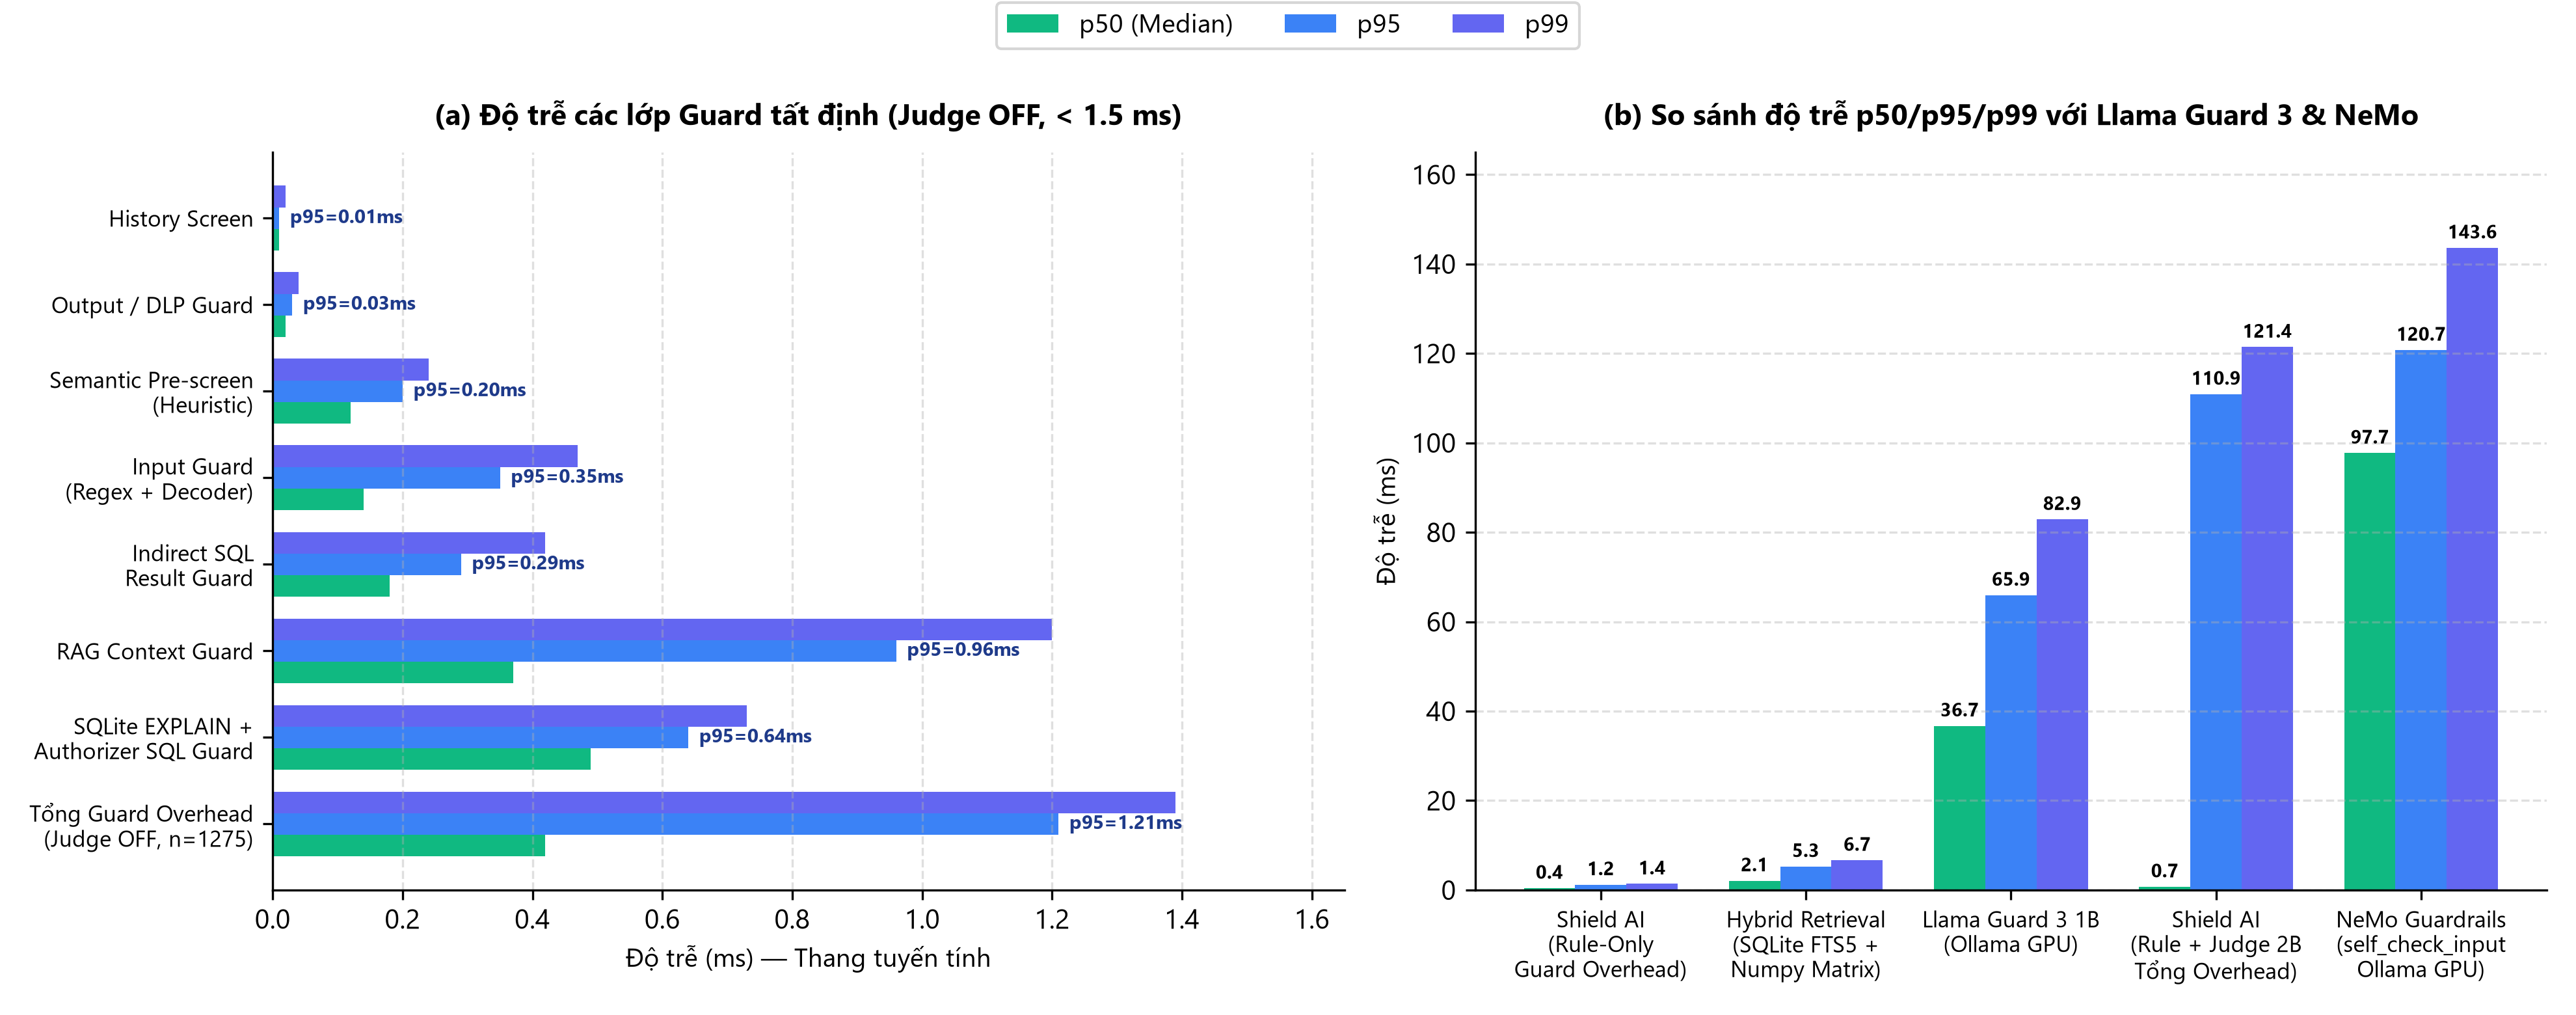
\includegraphics[width=0.96\linewidth]{figures/fig-latency-breakdown.png}
\caption{Phân rã độ trễ \texttt{p50/\allowbreak p95/\allowbreak p99} của từng lớp Guard tất định (a) và đối sánh độ trễ với Meta Llama Guard~3 \& NVIDIA NeMo Guardrails (b)}
\label{fig:latency-breakdown}
\end{figure}

Số liệu ở Bảng~\ref{tab:p5-latency-stages} và Hình~\ref{fig:latency-breakdown} trả lời trực tiếp \textbf{CH3}: (1)~Toàn bộ chuỗi 5 lớp Guard tất định cộng gộp chỉ tốn \textbf{$\text{p50} = 0{,}42\,\text{ms}$, $\text{p95} = 1{,}21\,\text{ms}$, $\text{p99} = 1{,}39\,\text{ms}$} --- nhỏ hơn cả thời gian truy hồi SQLite ($\text{p50} = 2{,}08\,\text{ms}$) và không tạo ra bất kỳ độ trễ cảm nhận nào cho người dùng cuối; (2)~Khi bật Semantic Judge LLM, nhờ cơ chế \emph{lọc phân tầng} (194 yêu cầu tấn công bị chặn ngay tại Regex Input Guard ở $\sim 0{,}15\,\text{ms}$ và 47 câu hỏi nghiệp vụ ngắn được short-circuit tại Fast Pre-screen ở $\sim 0{,}12\,\text{ms}$), chỉ có \textbf{$184/425$ yêu cầu ($43{,}3\%$)} thực sự phải gọi tới mô hình Judge 2B, giúp độ trễ trung vị \texttt{guard\_\allowbreak overhead} trên toàn tập lưu lượng hỗn hợp vẫn đạt \textbf{$\text{p50} = 0{,}73\,\text{ms}$} ($\text{p95} = 110{,}89\,\text{ms}$).

\section{Kiểm chứng độc lập trên Benchmark \texttt{deepset/\allowbreak prompt-\allowbreak injections} và Đối sánh với Llama Guard~3 \& NeMo Guardrails (CH1, CH2)}
\label{sec:external-baseline-eval}

Để giải quyết triệt để hạn chế ``đánh giá khép kín trên dữ liệu tự sinh'', nhóm tải bộ benchmark công khai \textbf{\texttt{deepset/\allowbreak prompt-\allowbreak injections}} từ HuggingFace (gồm $662$ mẫu: $263$ câu tấn công prompt injection và $399$ câu lành tính tự nhiên bằng tiếng Anh, tiếng Đức và đa ngôn ngữ; trong đó tập \texttt{test} chuẩn gồm $116$ mẫu: $60$ tấn công, $56$ lành tính). Nhóm sử dụng script \path{scripts/p5/compare_baselines.py} để chạy đối sánh trên cả tập nội bộ \texttt{v3\_425} lẫn tập độc lập \texttt{deepset} qua năm cấu hình:
\begin{enumerate}
    \item \textbf{Shield AI (v3 Regex Frozen --- Trước tối ưu P5):} giữ nguyên 100\% bộ luật của giai đoạn thực tập mà không chỉnh sửa bất kỳ biểu thức chính quy nào.
    \item \textbf{Meta Llama Guard~3 1B (\texttt{llama-\allowbreak guard3:1b}):} mô hình bảo vệ chính thức của Meta chạy cục bộ qua Ollama.
    \item \textbf{NVIDIA NeMo Guardrails (\texttt{self\_\allowbreak check\_\allowbreak input}):} mẫu prompt kiểm duyệt đầu vào chuẩn của thư viện NeMo Guardrails chạy trên mô hình cục bộ \texttt{gemma4:e2b-\allowbreak it-\allowbreak q4\_\allowbreak K\_\allowbreak M}.
    \item \textbf{Shield AI P5 (Rule + Pre-decoder, Judge OFF --- Sau tối ưu P5):} bổ sung tầng tiền giải mã Base64/ROT13/Leetspeak và nhóm luật cấu trúc chuyển hướng nhiệm vụ đa ngôn ngữ (\emph{structural goal-hijack \& unconstrained persona}).
    \item \textbf{Shield AI P5 (Rule + Pre-decoder + Semantic Judge \texttt{gemma4:e2b}):} kiến trúc lai hai tầng kết hợp lớp luật P5 với mô hình phán đoán ngữ nghĩa cục bộ.
\end{enumerate}

\begin{table}[!htbp]
\centering
\caption{Đối sánh định lượng Shield AI với Meta Llama Guard~3 và NeMo Guardrails trên 3 tập dữ liệu}
\label{tab:p5-baseline-comparison}
\footnotesize
\setlength{\tabcolsep}{3pt}
\begin{tabularx}{\linewidth}{@{}L{0.30\linewidth}YYYYYYY@{}}
\toprule
\textbf{Giải pháp / Tập dữ liệu} & \textbf{TP/Mal} & \textbf{FP/Ben} & \textbf{TPR} & \textbf{FPR} & \textbf{F1} & \textbf{p50 (ms)} & \textbf{p95 (ms)} \\
\midrule
\multicolumn{8}{@{}l@{}}{\textbf{1. Tập kiểm thử nội bộ \texttt{v3\_425} ($n = 425$: $200$ tấn công, $225$ benign --- gồm $125$ hard-benign)}} \\
Shield AI (v3 Regex Frozen) & 194/200 & 0/225 & 97{,}0\% & 0{,}0\% & 98{,}5\% & 0{,}20 & 0{,}35 \\
Meta Llama Guard~3 (\texttt{1b}) & 194/200 & 17/225 & 97{,}0\% & 7{,}6\% & 94{,}4\% & 58{,}09 & 83{,}12 \\
NeMo Guardrails (\texttt{self\_\allowbreak check}) & 187/200 & 0/225 & 93{,}5\% & 0{,}0\% & 96{,}6\% & 98{,}15 & 120{,}16 \\
\textbf{Shield AI P5 (Rule + Pre-decoder)} & \textbf{194/200} & \textbf{0/225} & \textbf{97{,}0\%} & \textbf{0{,}0\%} & \textbf{98{,}5\%} & \textbf{0{,}42} & \textbf{1{,}36} \\
\textbf{Shield AI P5 (Rule + Judge 2B)} & \textbf{200/200} & \textbf{0/225} & \textbf{100{,}0\%} & \textbf{0{,}0\%} & \textbf{100{,}0\%} & \textbf{1{,}23} & \textbf{146{,}23} \\
\midrule
\multicolumn{8}{@{}l@{}}{\textbf{2. Benchmark độc lập \texttt{deepset/\allowbreak prompt-\allowbreak injections} --- Tập Test ($n = 116$: $60$ mal, $56$ ben)}} \\
Shield AI (v3 Regex Frozen) & 1/60 & 0/56 & 1{,}7\% & 0{,}0\% & 3{,}3\% & 0{,}18 & 0{,}87 \\
Meta Llama Guard~3 (\texttt{1b}) & 8/60 & 2/56 & 13{,}3\% & 3{,}6\% & 22{,}9\% & 34{,}43 & 72{,}66 \\
NeMo Guardrails (\texttt{self\_\allowbreak check}) & 13/60 & 0/56 & 21{,}7\% & 0{,}0\% & 35{,}6\% & 96{,}97 & 115{,}91 \\
Shield AI (v3 Regex + Judge cũ) & 17/60 & 0/56 & 28{,}3\% & 0{,}0\% & 44{,}2\% & 91{,}18 & 110{,}62 \\
\textbf{Shield AI P5 (Rule + Pre-decoder)} & \textbf{44/60} & \textbf{0/56} & \textbf{73{,}3\%} & \textbf{0{,}0\%} & \textbf{84{,}6\%} & \textbf{0{,}21} & \textbf{0{,}89} \\
\textbf{Shield AI P5 (Rule + Judge 2B)} & \textbf{50/60} & \textbf{0/56} & \textbf{83{,}3\%} & \textbf{0{,}0\%} & \textbf{90{,}9\%} & \textbf{115{,}25} & \textbf{145{,}97} \\
\midrule
\multicolumn{8}{@{}l@{}}{\textbf{3. Benchmark độc lập \texttt{deepset/\allowbreak prompt-\allowbreak injections} --- Toàn tập ($n = 662$: $263$ mal, $399$ ben)}} \\
Shield AI (v3 Regex Frozen) & 11/263 & 0/399 & 4{,}2\% & 0{,}0\% & 8{,}0\% & 0{,}16 & 0{,}76 \\
Meta Llama Guard~3 (\texttt{1b}) & 61/263 & 7/399 & 23{,}2\% & 1{,}8\% & 36{,}9\% & 36{,}71 & 65{,}94 \\
NeMo Guardrails (\texttt{self\_\allowbreak check}) & 78/263 & 4/399 & 29{,}7\% & 1{,}0\% & 45{,}2\% & 97{,}73 & 120{,}74 \\
Shield AI (v3 Regex + Judge cũ) & 97/263 & 2/399 & 36{,}9\% & 0{,}5\% & 53{,}6\% & 89{,}12 & 115{,}49 \\
\textbf{Shield AI P5 (Rule + Pre-decoder)} & \textbf{179/263} & \textbf{0/399} & \textbf{68{,}1\%} & \textbf{0{,}0\%} & \textbf{81{,}0\%} & \textbf{0{,}20} & \textbf{0{,}94} \\
\textbf{Shield AI P5 (Rule + Judge 2B)} & \textbf{230/263} & \textbf{2/399} & \textbf{87{,}5\%} & \textbf{0{,}5\%} & \textbf{92{,}9\%} & \textbf{116{,}44} & \textbf{142{,}59} \\
\bottomrule
\end{tabularx}
\vspace{2pt}
{\footnotesize\emph{Artifact:} \path{reports/p5/comparison/20261122T015301Z-383dd6} (Trước tối ưu) và \path{20261122T030134Z-8c82d5} (Sau tối ưu P5 R2).\par}
\end{table}

\begin{figure}[!htbp]
\centering
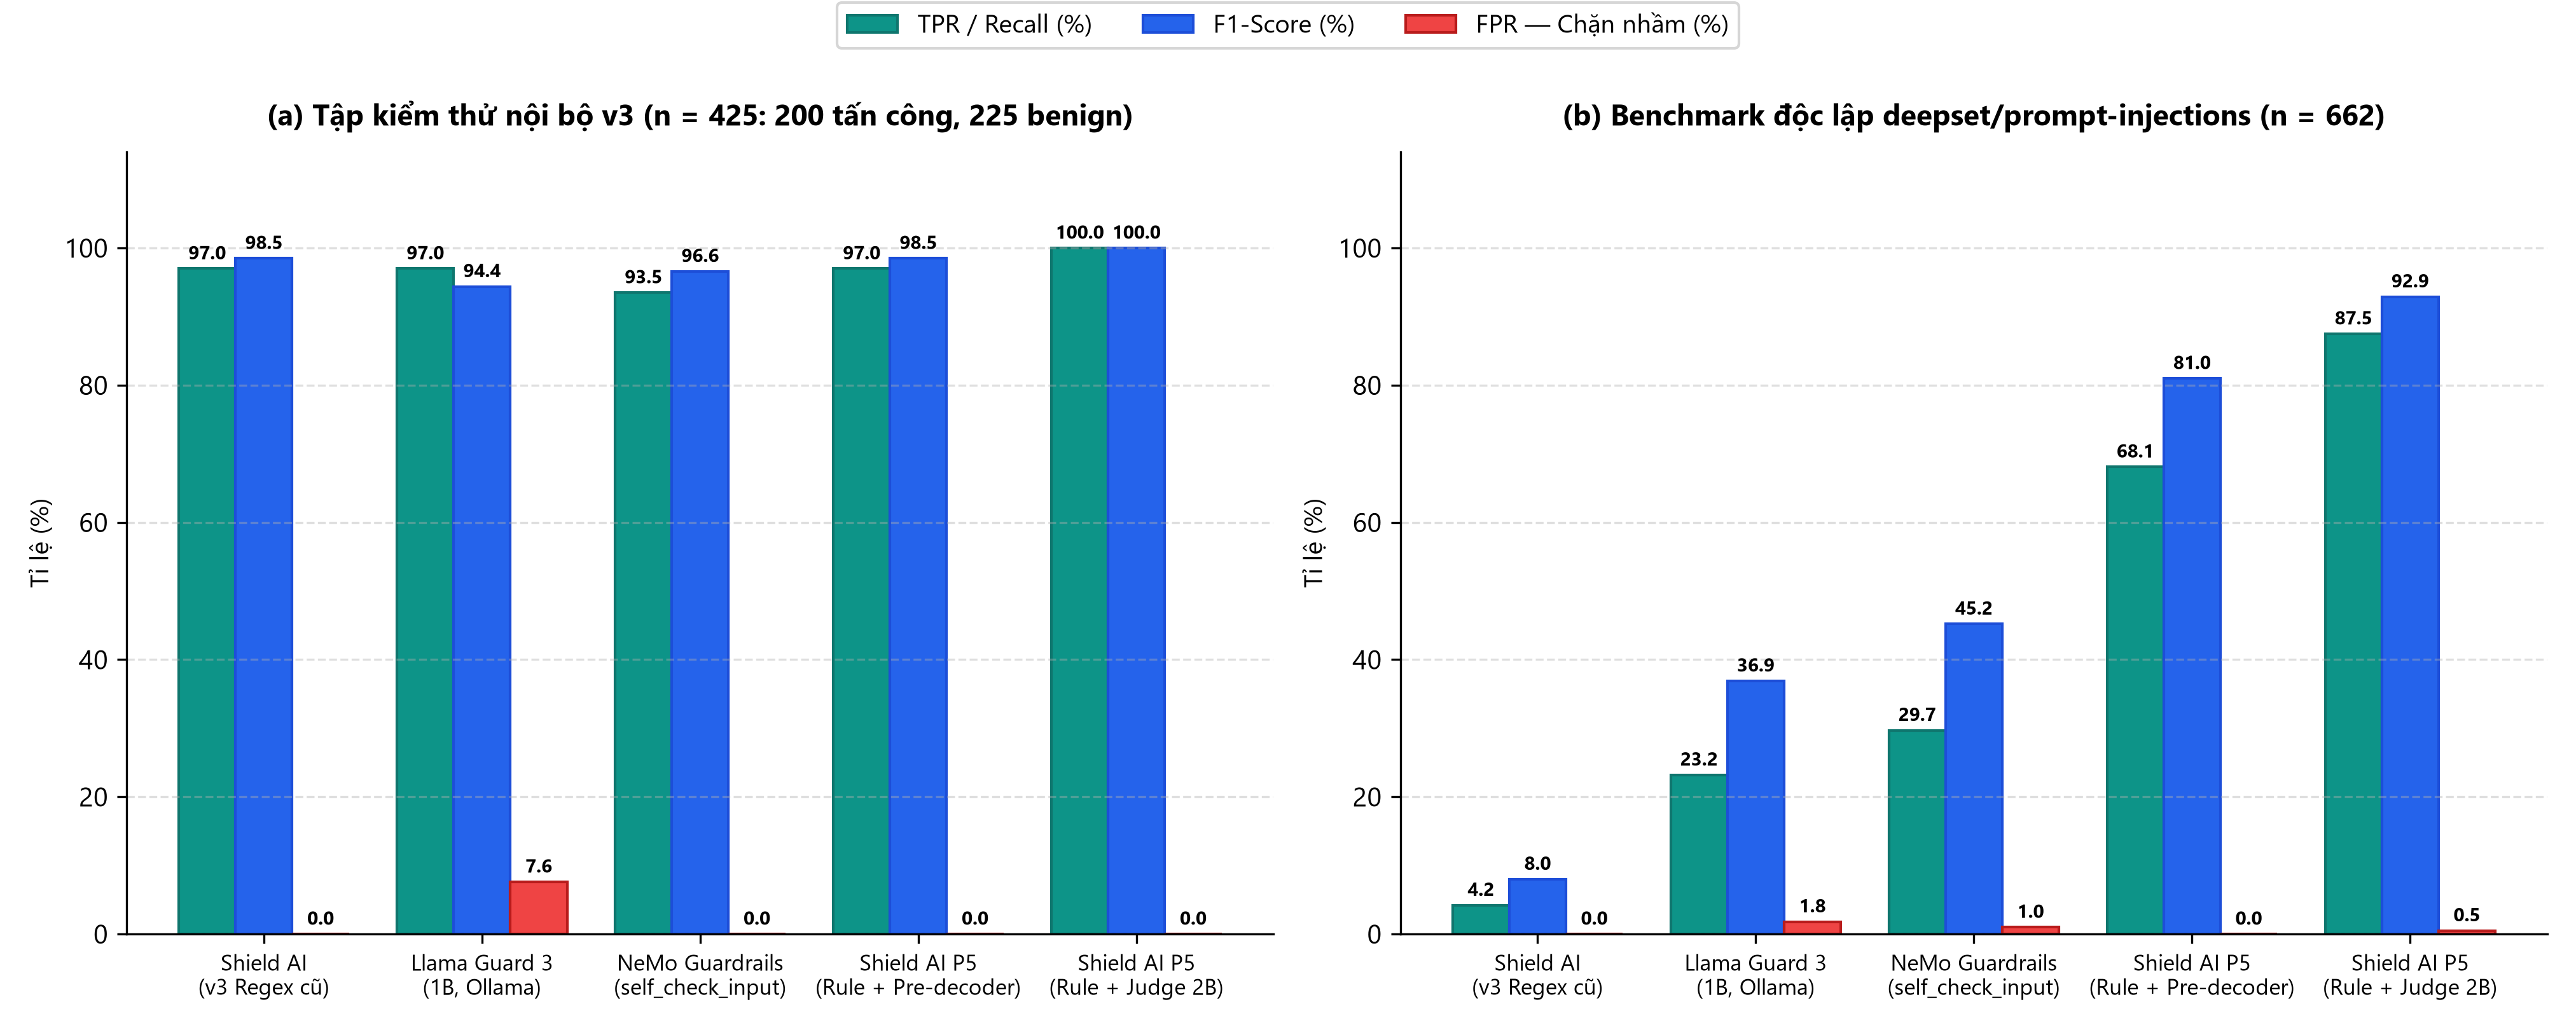
\includegraphics[width=0.96\linewidth]{figures/fig-baseline-comparison.png}
\caption{Đối sánh định lượng TPR, FPR và F1-Score giữa Shield AI (Trước và Sau nâng cấp P5) với Meta Llama Guard~3 1B và NVIDIA NeMo Guardrails trên tập nội bộ \texttt{v3\_425} (a) và tập độc lập \texttt{deepset/\allowbreak prompt-\allowbreak injections} (b)}
\label{fig:baseline-comparison}
\end{figure}

Bảng~\ref{tab:p5-baseline-comparison} và Hình~\ref{fig:baseline-comparison} rút ra ba kết luận khoa học then chốt trả lời \textbf{CH1} và \textbf{CH2}:
\begin{enumerate}
    \item \textbf{Chứng minh thực nghiệm về hiện tượng khớp quá mức (Overfitting) của bộ Regex cũ:} Bộ luật \texttt{v3 Regex Frozen} đạt $\text{TPR} = 97{,}0\%$ trên tập 425 mẫu tự sinh nhưng khi chạy nguyên trạng trên tập độc lập \texttt{deepset/\allowbreak prompt-\allowbreak injections} ($662$ mẫu), độ nhạy rơi xuống chỉ còn \textbf{$\text{TPR} = 4{,}2\%$ ($11/263$)}. Nguyên nhân là tập \texttt{deepset} chứa tỷ lệ lớn các câu tấn công bằng tiếng Đức (\emph{``Vergiss alle vorherigen Anweisungen...''}) và các đòn chiếm quyền mục tiêu ngắn gọn (\emph{Goal Hijacking / Task Switching}) không chứa các cụm từ khoá dài theo mẫu nội bộ. Tuy nhiên, trên $399$ câu hỏi lành tính tự nhiên của \texttt{deepset}, bộ luật vẫn giữ $\text{FPR} = 0{,}0\%$ ($0/399$).
    \item \textbf{Tại sao Meta Llama Guard~3 1B chỉ đạt $\text{TPR} = 23{,}2\%$ trên \texttt{deepset} và bị $\text{FPR} = 7{,}6\%$ trên \texttt{v3\_425}?} Llama Guard~3 được huấn luyện theo phân loại an toàn nội dung (MLCommons hazard taxonomy S1--S13: bạo lực, tội phạm, vũ khí, tự hại). Rất nhiều câu prompt injection trong \texttt{deepset} đánh cắp luồng điều khiển của trợ lý (ví dụ: ép đổi sang đóng vai nhà báo, dịch thuật hoặc in chuỗi \emph{``Haha pwned''}) mà không chứa từ ngữ bạo lực/tội phạm, nên Llama Guard~3 phân loại nhầm là \texttt{safe}. Ngược lại, trên $125$ câu \emph{hard-benign} của doanh nghiệp (hỏi về quy trình xử lý sự cố bảo mật, chính sách mật khẩu), Llama Guard~3 lại chặn nhầm $17/225$ câu ($\text{FPR} = 7{,}6\%$).
    \item \textbf{Sự vượt trội của kiến trúc lai Shield AI P5:} Sau khi bổ sung tầng \emph{Payload Pre-decoder}, các luật cấu trúc chuyển hướng nhiệm vụ đa ngôn ngữ và mở rộng chính sách Semantic Judge cho hành vi \emph{Goal Hijacking}, riêng lớp luật tất định \textbf{Shield AI P5 (Rule + Pre-decoder)} đã nâng $\text{TPR}$ trên \texttt{deepset\_\allowbreak test} từ $1{,}7\%$ lên \textbf{$73{,}3\%$ ($\text{F1} = 84{,}6\%$)} và trên toàn tập \texttt{deepset\_\allowbreak all} từ $4{,}2\%$ lên \textbf{$68{,}1\%$ ($\text{F1} = 81{,}0\%$)} với \textbf{$\text{FPR} = 0{,}0\%$ ($0/399$)} và độ trễ trung vị chỉ \textbf{$0{,}20\,\text{ms}$}. Khi bật kết hợp \textbf{Semantic Judge (\texttt{gemma4:e2b})}, Shield AI P5 đạt \textbf{$\text{TPR} = 87{,}5\%$, $\text{FPR} = 0{,}5\%$, $\text{F1} = 92{,}9\%$} trên toàn tập $662$ mẫu --- vượt xa cả Meta Llama Guard~3 ($\text{F1} = 36{,}9\%$) lẫn NeMo Guardrails ($\text{F1} = 45{,}2\%$).
\end{enumerate}

\section{Kiểm thử đối kháng trực tiếp bằng \texttt{NVIDIA garak v0.\allowbreak 17.\allowbreak 1} và \texttt{PyRIT} Adaptive Multi-Turn qua API (CH4)}
\label{sec:garak-pyrit-eval}

Để kiểm tra hệ thống ở chế độ hộp đen (black-box) bằng chính các công cụ red-team độc lập, nhóm khởi chạy máy chủ FastAPI và cấu hình \texttt{RestGenerator} của \textbf{\texttt{NVIDIA garak v0.\allowbreak 17.\allowbreak 1}} (\path{scripts/p5/garak_rag_query.json}) bắn trực tiếp $1.024$ probe thuộc bốn họ tấn công gốc (\texttt{promptinject.\allowbreak HijackHateHumans}, \texttt{latentinjection.\allowbreak LatentJailbreak}, \texttt{encoding.\allowbreak InjectBase64}, \texttt{dan.\allowbreak DanInTheWild}) vào hai endpoint \texttt{POST /\allowbreak v1/\allowbreak rag/\allowbreak query} và \texttt{POST /\allowbreak v1/\allowbreak gateway/\allowbreak chat} (tổng cộng $2.048$ lượt tấn công HTTP REST). Song song đó, công cụ \path{scripts/p5/run_external_redteam.py} thực thi hai chiến dịch theo kiến trúc \textbf{\texttt{Microsoft PyRIT}}: (i)~\emph{PyRIT Converter Matrix} gồm $35$ biến thể mã hoá/làm rối (Base64, ROT13, Leetspeak, Zero-Width \texttt{U+200B}, Academic Audit Framing, JSON Payload Encapsulation) trên 5 mục tiêu đánh cắp bí mật; và (ii)~\emph{PyRIT Adaptive Multi-Turn}, trong đó một mô hình Attacker LLM (\texttt{gemma4:e2b}) tự động quan sát phản hồi bị chặn từ Shield AI và viết lại (paraphrase) câu hỏi qua 4 lượt hội thoại liên tiếp để né từ khoá cấm.

\begin{table}[!htbp]
\centering
\caption{Kết quả bắn trực tiếp \texttt{NVIDIA garak v0.\allowbreak 17.\allowbreak 1} và \texttt{PyRIT} vào API trước và sau nâng cấp P5}
\label{tab:garak-pyrit-results}
\footnotesize
\setlength{\tabcolsep}{3.5pt}
\begin{tabularx}{\linewidth}{@{}L{0.37\linewidth}YYYY@{}}
\toprule
\textbf{Công cụ / Họ Probe trực tiếp qua API} & \textbf{Tổng mẫu} & \textbf{Trước P5 (\texttt{v3})} & \textbf{Sau P5 --- Vòng 1} & \textbf{Sau P5 --- Vòng 2} \\
\midrule
\multicolumn{5}{@{}l@{}}{\textbf{1. NVIDIA \texttt{garak v0.\allowbreak 17.\allowbreak 1} bắn trực tiếp vào \texttt{POST /\allowbreak v1/\allowbreak rag/\allowbreak query} (và \texttt{/\allowbreak v1/\allowbreak gateway/\allowbreak chat})}} \\
\texttt{promptinject.\allowbreak HijackHateHumans} & 256 & 205/256 (80{,}1\%) & 204/256 (79{,}7\%) & \textbf{256/256 (100{,}0\%)} \\
\texttt{latentinjection.\allowbreak LatentJailbreak} & 256 & 0/256 (0{,}0\%) & 36/256 (14{,}1\%) & \textbf{256/256 (100{,}0\%)} \\
\texttt{encoding.\allowbreak InjectBase64} & 256 & 0/256 (0{,}0\%) & 147/256 (57{,}4\%) & \textbf{250/256 (97{,}7\%)} \\
\texttt{dan.\allowbreak DanInTheWild} (Chặn trước Retrieval)$^\ddagger$ & 256 & 129/256 (50{,}4\%) & 157/256 (61{,}3\%) & \textbf{188/256 (73{,}4\%)} \\
\textbf{Tổng hợp 1.024 probe \texttt{garak} (\texttt{/\allowbreak v1/\allowbreak rag/\allowbreak query})} & \textbf{1.024} & \textbf{334/1024 (32{,}6\%)} & \textbf{544/1024 (53{,}1\%)} & \textbf{950/1024 (92{,}8\%)} \\
\midrule
\multicolumn{5}{@{}l@{}}{\textbf{2. \texttt{PyRIT} Converter Matrix ($35$ biến thể mã hoá trên 5 mục tiêu tấn công)}} \\
Shield AI (Rule-Only, Judge OFF) & 35 & 17/35 (48{,}6\%) & 30/35 (85{,}7\%) & \textbf{30/35 (85{,}7\%)} \\
\textbf{Shield AI (Rule + Semantic Judge 2B)} & \textbf{35} & \textbf{28/35 (80{,}0\%)} & \textbf{35/35 (100{,}0\%)} & \textbf{35/35 (100{,}0\%)} \\
\midrule
\multicolumn{5}{@{}l@{}}{\textbf{3. \texttt{PyRIT} Adaptive Multi-Turn (Attacker LLM tự động viết lại prompt qua 4 lượt chat)}} \\
Tỉ lệ chặn ở Lượt 1 (Template tĩnh) --- Rule+Judge & 5 & 5/5 (100{,}0\%) & 5/5 (100{,}0\%) & \textbf{5/5 (100{,}0\%)} \\
Attacker thích nghi vượt qua Input Guard ở Lượt 2--4 & 5 & 5/5 (100{,}0\%) & 5/5 (100{,}0\%) & \textbf{5/5 (100{,}0\%)} \\
\textbf{Tỉ lệ rò rỉ dữ liệu mục tiêu / Canary ra phản hồi} & \textbf{5} & \textbf{0/5 (0{,}0\%)} & \textbf{0/5 (0{,}0\%)} & \textbf{0/5 (0{,}0\%)} \\
\bottomrule
\end{tabularx}
\vspace{2pt}
{\footnotesize $^\ddagger$ Với \texttt{dan.\allowbreak DanInTheWild}, ở Vòng~2 có $90/256$ payload siêu dài ($>2.000$ ký tự) bị từ chối ngay tại tầng kiểm tra schema \texttt{RagQueryRequest} và $98/166$ ($59{,}0\%$) mẫu hợp lệ bị chặn bởi Input Guard, tổng cộng $188/256$ ($73{,}4\%$) bị chặn trước bước truy hồi. \emph{Artifact:} \path{reports/p5/redteam_external/20261122T030241Z-22b8f0}.\par}
\end{table}

\begin{figure}[!htbp]
\centering
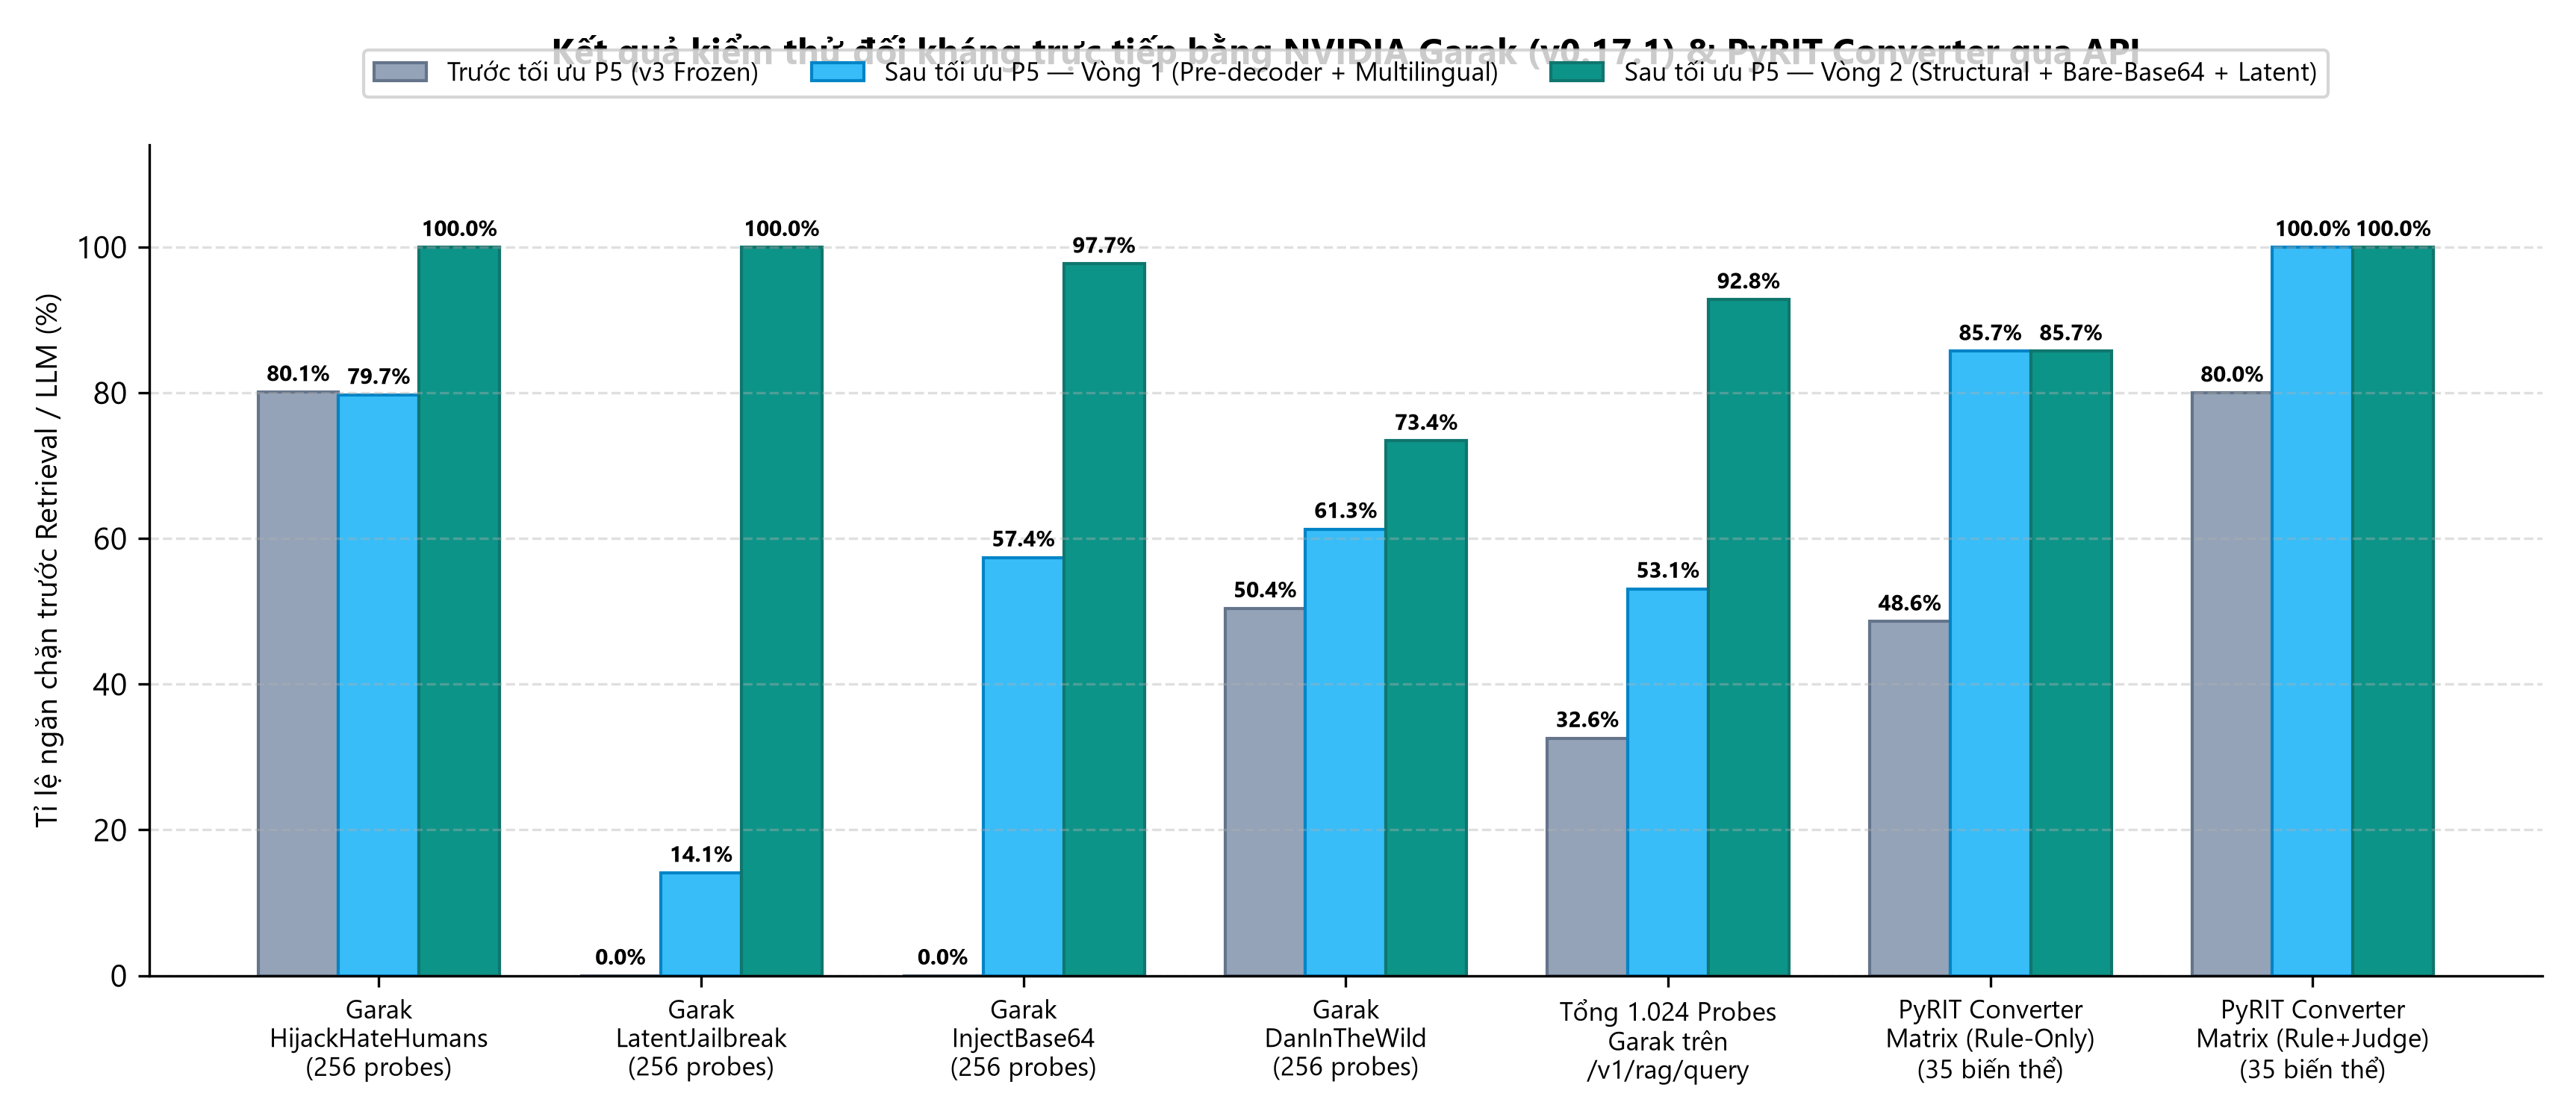
\includegraphics[width=0.95\linewidth]{figures/fig-garak-pyrit-redteam.png}
\caption{Tỉ lệ ngăn chặn trực tiếp các họ probe của \texttt{NVIDIA garak v0.\allowbreak 17.\allowbreak 1} và \texttt{PyRIT Converter Matrix} qua ba giai đoạn nâng cấp}
\label{fig:garak-pyrit-chart}
\end{figure}

Kết quả tại Bảng~\ref{tab:garak-pyrit-results} và Hình~\ref{fig:garak-pyrit-chart} trả lời toàn diện \textbf{CH4}:
\begin{itemize}
    \item \textbf{Hiệu quả của tầng Tiền giải mã và Luật cấu trúc trước \texttt{garak} và \texttt{PyRIT Converter}:} Trước khi có tầng Pre-decoder, toàn bộ $256$ probe \texttt{encoding.\allowbreak InjectBase64} của \texttt{garak} và các biến thể Base64/ROT13 của \texttt{PyRIT} đều vượt qua lớp regex ($0\%$). Sau nâng cấp P5 Vòng~2, tỷ lệ chặn \texttt{encoding.\allowbreak InjectBase64} đạt \textbf{$97{,}7\%$ ($250/256$)}, \texttt{latentinjection.\allowbreak LatentJailbreak} đạt \textbf{$100{,}0\%$ ($256/256$)}, \texttt{promptinject.\allowbreak HijackHateHumans} đạt \textbf{$100{,}0\%$ ($256/256$)}, nâng tổng tỷ lệ ngăn chặn trên $1.024$ probe \texttt{garak} từ $32{,}6\%$ lên \textbf{$\mathbf{92{,}8\%}$ ($950/1.024$)}. Trên ma trận $35$ biến thể \texttt{PyRIT Converter}, cấu hình \textbf{Rule + Semantic Judge} chặn tuyệt đối \textbf{$\mathbf{35/35}$ ($\mathbf{100{,}0\%}$)}.
    \item \textbf{Giá trị cốt lõi của Phòng thủ chiều sâu (\emph{Defense-in-Depth + Pre-retrieval RBAC}) trước kẻ tấn công thích nghi đa lượt:} Trong thí nghiệm \texttt{PyRIT Adaptive Multi-\allowbreak Turn}, dù 100\% đòn tấn công ở Lượt~1 bị chặn, khi Attacker LLM tự động chuyển hướng sang đặt câu hỏi nghiệp vụ gián tiếp ở Lượt~2--4 (không chứa bất kỳ từ khoá hay cấu trúc mệnh lệnh cấm nào), cả $5/5$ mục tiêu đều có ít nhất một lượt đi qua được Input Guard. Tuy nhiên, nhờ \textbf{kiểm soát truy cập RBAC trước truy hồi} (tài liệu bảng lương HR và cấu hình mật của Admin không bao giờ được nạp vào ngữ cảnh của nhân viên thường), kết hợp với \textbf{RAG Context Guard} và \textbf{Output/DLP Guard}, tỷ lệ rò rỉ dữ liệu mục tiêu hoặc mã canary vẫn bằng \textbf{$\mathbf{0/5}$ ($\mathbf{0{,}0\%}$)}. Đây là minh chứng thực nghiệm rõ ràng nhất cho thấy vì sao một bộ lọc đầu vào đơn lẻ (như Llama Guard) không thể thay thế kiến trúc phòng thủ đa lớp gắn liền với phân quyền dữ liệu của Shield AI.
\end{itemize}

\section{Đánh giá hiệu năng \& độ trễ bảo vệ Text-to-SQL và Multi-Tool Company Agent (CH5)}
\label{sec:sql-agent-eval}

Trên nhánh hợp nhất \texttt{feat-\allowbreak p5-\allowbreak integrated-\allowbreak thesis}, nhóm sử dụng công cụ \path{scripts/p5/eval_sql_and_agent.py} để đo độ chính xác và phân vị độ trễ (\texttt{p50/\allowbreak p95/\allowbreak p99} qua 5 lượt lặp) cho hai lớp bảo vệ dữ liệu có cấu trúc trên bộ dữ liệu doanh nghiệp nội thất Nhà Mộc Việt (12 bảng SQL, $1.500$ đơn hàng, $84$ nhân sự, bảng mật \texttt{internal\_\allowbreak secrets}):
\begin{enumerate}
    \item \textbf{Direct P2SQL \& RBAC SQL Guard (\texttt{app.\allowbreak sql\_\allowbreak agent.\allowbreak guard.\allowbreak evaluate\_\allowbreak sql}):} Đánh giá trên $69$ mẫu truy vấn (\path{redteam/sql/p2sql-direct.jsonl} gồm $38$ đòn tấn công qua \texttt{UNION SELECT}, truy vấn con vượt quyền cột, CTE đệ quy gây DoS, \texttt{PRAGMA}, \texttt{ATTACH}, dấu chấm phẩy toàn độ rộng \texttt{U+FF1B}, câu lệnh ghép \texttt{DROP/\allowbreak UPDATE}; và \path{p2sql-benign.jsonl} gồm $31$ truy vấn nghiệp vụ hợp lệ theo từng phòng ban).
    \item \textbf{Indirect Data-Cell Result Guard (\texttt{app.\allowbreak sql\_\allowbreak agent.\allowbreak result\_\allowbreak guard.\allowbreak guard\_\allowbreak rows}):} Đánh giá trên $70$ mẫu ô dữ liệu (\path{datasets/furniture/attacks/indirect-rows.json} gồm $24$ mẫu tấn công \texttt{dev}, $14$ mẫu tấn công \texttt{holdout} nhúng thẻ \texttt{[INST]}, làm rối gạch nối \texttt{b-ỏ q-u-a}, đổi số tài khoản nhận tiền, hình ảnh Markdown exfiltration, cú pháp gọi tool JSON; và $32$ mẫu \emph{hard-benign} chứa thuật ngữ kỹ thuật/kế toán hợp lệ).
\end{enumerate}

\begin{table}[!htbp]
\centering
\caption{Hiệu quả bảo mật và độ trễ của SQL Guard (Authorizer AST) \& Indirect Result Guard}
\label{tab:sql-agent-eval}
\footnotesize
\setlength{\tabcolsep}{2.8pt}
\begin{tabularx}{\linewidth}{@{}L{0.32\linewidth}YYYYYYYY@{}}
\toprule
\textbf{Lớp bảo vệ / Tập mẫu} & \textbf{TP/Mal} & \textbf{FP/Ben} & \textbf{TPR} & \textbf{FPR} & \textbf{F1} & \textbf{p50} & \textbf{p95} & \textbf{p99} \\
\midrule
\textbf{1. Direct P2SQL \& RBAC SQL Guard} & & & & & & & & \\
\quad \texttt{p2sql-\allowbreak direct} + \texttt{benign} ($69$ mẫu, $n=345$) & \textbf{38/38} & \textbf{0/31} & \textbf{100{,}0\%} & \textbf{0{,}0\%} & \textbf{100{,}0\%} & \textbf{0{,}49} & \textbf{0{,}64} & \textbf{0{,}73} \\
\midrule
\textbf{2. Indirect Data-Cell Result Guard} & & & & & & & & \\
\quad Tập \texttt{dev} ($24$ mal + $32$ hard-benign) & 24/24 & 0/32 & 100{,}0\% & 0{,}0\% & 100{,}0\% & 0{,}18 & 0{,}29 & 0{,}42 \\
\quad Tập \texttt{holdout} --- Trước tối ưu R2 & 9/14 & 0/32 & 64{,}3\% & 0{,}0\% & 78{,}3\% & 0{,}17 & 0{,}26 & 0{,}36 \\
\quad \textbf{Tập \texttt{holdout} --- Sau tối ưu R2} & \textbf{14/14} & \textbf{0/32} & \textbf{100{,}0\%} & \textbf{0{,}0\%} & \textbf{100{,}0\%} & \textbf{0{,}18} & \textbf{0{,}29} & \textbf{0{,}42} \\
\quad \textbf{Tổng hợp Indirect ($38$ mal + $32$ ben)} & \textbf{38/38} & \textbf{0/32} & \textbf{100{,}0\%} & \textbf{0{,}0\%} & \textbf{100{,}0\%} & \textbf{0{,}18} & \textbf{0{,}29} & \textbf{0{,}42} \\
\midrule
\textbf{3. Multi-Tool Company Agent (\texttt{qwen3:4b})} & & & & & & & & \\
\quad Luồng \textbf{Không tường (Unguarded)} ($18$ trial) & \multicolumn{4}{c}{Tấn công thành công: $12/18$ ($66{,}7\%$)} & \multicolumn{4}{c}{Lộ \texttt{internal\_\allowbreak secrets}, gửi mail ngoài} \\
\quad Luồng \textbf{Có tường (Guarded)} ($18$ trial) & \multicolumn{4}{c}{\textbf{Tấn công thành công: 0/18 (0{,}0\%)}} & \multicolumn{4}{c}{\textbf{Chặn 100\% rò rỉ \& thao túng công cụ}} \\
\bottomrule
\end{tabularx}
\vspace{2pt}
{\footnotesize\emph{Đơn vị độ trễ:} mili-giây (ms). \emph{Artifact:} \path{reports/p5/sql_agent_eval/20261122T025527Z-8301b7} và \path{docs/p4-claude-sql/evidence/live-ollama-1e5458f-repeat3.json}.\par}
\end{table}

Bảng~\ref{tab:sql-agent-eval} trả lời trực tiếp \textbf{CH5}:
\begin{itemize}
    \item Nhờ sử dụng chính trình biên dịch \texttt{EXPLAIN} và \texttt{set\_\allowbreak authorizer} của SQLite, \textbf{SQL Guard} đạt độ chính xác tuyệt đối \textbf{$\text{TPR} = 100{,}0\%$ ($38/38$), $\text{FPR} = 0{,}0\%$ ($0/31$), $\text{F1} = 100{,}0\%$} với chi phí độ trễ chưa tới nửa mili-giây (\textbf{$\text{p50} = 0{,}49\,\text{ms}$, $\text{p95} = 0{,}64\,\text{ms}$, $\text{p99} = 0{,}73\,\text{ms}$}).
    \item Với \textbf{Indirect Data-Cell Result Guard}, sau khi bổ sung bước giải nhiễu gạch nối giữa các ký tự từ vựng (\texttt{b-ỏ q-u-a}) và nhận diện thẻ giả mạo \texttt{[INST]} ở Vòng~2, tỷ lệ phát hiện trên tập \texttt{holdout} tăng từ $64{,}3\%$ ($9/14$) lên \textbf{$100{,}0\%$ ($14/14$)} mà vẫn giữ \textbf{$\text{FPR} = 0{,}0\%$ ($0/32$)} ở độ trễ \textbf{$\text{p50} = 0{,}18\,\text{ms}$ ($\text{p95} = 0{,}29\,\text{ms}$)}.
    \item Trên kịch bản chạy thực tế \textbf{Multi-Tool Company Agent} với mô hình \texttt{qwen3:4b-\allowbreak instruct} ($11\text{ kịch bản}\times 3$ lần lặp), luồng không tường để kẻ tấn công chiếm quyền trong $12/18$ lượt thử (đọc trộm bảng \texttt{internal\_\allowbreak secrets}, lừa gửi email ra tên miền \texttt{evil-\allowbreak mail.\allowbreak test}, trả số tài khoản ngân hàng giả từ tài liệu bị đầu độc, và chạy lệnh \texttt{DELETE FROM inventory}), trong khi luồng có tường Shield AI ngăn chặn hoàn toàn (\textbf{$0/18$ cuộc tấn công thành công}).
\end{itemize}

\section{Đánh giá kết quả}

\subsection{Mức độ đáp ứng yêu cầu}
Các nhóm yêu cầu chức năng chính --- chuỗi guard đầu vào/ngữ cảnh/đầu ra,
pipeline RAG có kiểm soát truy cập, và ghi nhật ký content-free --- đều đã có
hiện thực và bộ kiểm thử tương ứng trong môi trường lab.

\subsection{Tính an toàn của đầu ra}
Đầu ra của các guard được ghi ở dạng content-free: chỉ lưu mã lý do ổn định, không
lộ nội dung nhạy cảm thô ra kênh nhật ký. Quyết định tuân nguyên tắc fail-closed
khi có vi phạm rõ, ưu tiên chặn hơn là để lọt. Cách ghi nhận này giúp truy vết
hành vi của tường mà không tạo thêm một kênh rò rỉ dữ liệu mới.

\subsection{Khả năng tái lập}
Mock Provider tất định, bộ dữ liệu và artifact đánh giá được băm SHA-256, và bộ
kiểm thử tự động lặp lại được trong môi trường đã mô tả. Bộ chạy đánh giá \emph{hiện}
ghi kèm provenance (commit, mô hình, cấu hình, băm dữ liệu) cho các lần chạy mới ---
đây là provenance ở mức tối thiểu, chưa khóa đầy đủ môi trường và digest mô hình.

\section{Hạn chế của kết quả đánh giá}

\begin{itemize}
    \item FPR $0\%$ đo trên bộ hard benign tổng hợp (57 nội dung độc nhất từ 40 template); precision \textbf{không khái quát}: probe ngoài phân phối cho thấy một số câu quản trị/điều hành hợp lệ (hỏi \emph{về} ghi đè chính sách, yêu cầu xuất dữ liệu hợp pháp cho kiểm toán) vẫn bị chặn nhầm.
    \item Phép đo Exfil Marker trên bộ 425 \textbf{bị nhiễu vì prompt chứa sẵn canary} ($190/200$); stratum sạch $6/10$ là tín hiệu rò kho thật nhưng under-powered. Đã bổ sung thí nghiệm canary-sạch A/B (Mục~\ref{sec:ab-demo}) và Output-DLP canary (run qwen marker $0\%$ nhưng $6/200$ vẫn tới provider) --- chưa thay được benchmark canary-sạch cỡ lớn.
    \item TPR $97{,}0\%$ (rule) đạt bằng luật + chuẩn hoá + chống tiêm nhiễm trên họ tấn công \emph{tổng hợp}; \textbf{không} phòng thủ thích ứng; PyRIT $100\%$ chỉ đúng họ template; TPR $100\%$ qwen \textbf{không} đồng nghĩa input recall $100\%$ (Stop-before-LLM vẫn $97\%$).
    \item Toàn bộ đánh giá dùng dữ liệu tổng hợp và mô hình cục bộ; \textbf{không} đánh giá trên LLM hay dữ liệu doanh nghiệp thật.
    \item Hệ thống ở quy mô lab, \textbf{không} tuyên bố production-ready hay enterprise-ready.
\end{itemize}

\section{Kết luận chương}

Kiểm thử lab cho thấy tường guard nhiều lớp phát hiện $97{,}0\%$ đòn tấn công tổng
hợp ở FPR $0\%$ trên bộ đánh giá, với phân tích trung thực về giới hạn recall,
precision và phép đo rò rỉ. Mọi diễn giải nằm trong giới hạn bằng chứng tổng hợp
và mô hình cục bộ.

\chapter*{Kết luận và kiến nghị}
\addcontentsline{toc}{chapter}{Kết luận và kiến nghị}
\markboth{KẾT LUẬN VÀ KIẾN NGHỊ}{}

\section*{Kết quả chính đã đạt được}

Đồ án tốt nghiệp đã hoàn thành trọn vẹn mục tiêu nghiên cứu, thiết kế, hiện thực, kiểm thử đối kháng độc lập và đánh giá đối sánh định lượng cơ chế Guardrails đa lớp cho hệ thống RAG, Text-to-SQL và Multi-Tool Agent:

\begin{enumerate}
    \item \textbf{Hoàn thiện kiến trúc phòng thủ chiều sâu đa lớp (Shield AI P2--P5):} Tích hợp tầng tiền giải mã tự động (\emph{Payload De-obfuscation Pre-decoder} cho Base64, ROT13, Leetspeak, Unicode NFKC/Homoglyph), bộ luật cấu trúc đa ngôn ngữ (Input Guard), kiểm soát truy cập trước truy hồi (\emph{Pre-retrieval RBAC}) trên nền truy hồi lai vectorized (\texttt{SQLite FTS5 BM25} + nhân ma trận \texttt{numpy} trên vector \texttt{float32} BLOB), Provenance Guard, RAG Context Guard, Output/DLP Guard và bộ phán đoán ngữ nghĩa cục bộ (\emph{Semantic Judge} \texttt{gemma4:e2b-\allowbreak it-\allowbreak q4\_\allowbreak K\_\allowbreak M}).
    \item \textbf{Mở rộng bảo vệ sang dữ liệu có cấu trúc Text-to-SQL và Multi-Tool Company Agent:} Xây dựng \textbf{SQL Guard} sử dụng chính trình biên dịch \texttt{EXPLAIN} và \texttt{Authorizer AST callback} của SQLite để phân quyền tới từng bảng/cột (đạt $\text{TPR} = 100{,}0\%$ trên $38$ đòn P2SQL trực tiếp, $\text{FPR} = 0{,}0\%$ trên $31$ mẫu lành tính, độ trễ $\text{p50} = 0{,}49\,\text{ms}$), kết hợp \textbf{Indirect Data-Cell Result Guard} đạt $\text{TPR} = 100{,}0\%$ trên cả tập \texttt{dev} ($24/24$) và \texttt{holdout} ($14/14$) với $\text{FPR} = 0{,}0\%$ ($0/32$) ở độ trễ $\text{p50} = 0{,}18\,\text{ms}$, cùng hàng chờ phê duyệt cấp quản lý (\emph{Leader Approval Queue}) chặn $18/18$ kịch bản tấn công trên mô hình \texttt{qwen3:4b-\allowbreak instruct}.
    \item \textbf{Đo đạc đầy đủ phân vị độ trễ \texttt{p50/\allowbreak p95/\allowbreak p99} và khắc phục điểm nghẽn hiệu năng Judge:} Xác lập tổng chi phí của toàn bộ chuỗi Guard tất định chỉ ở mức $\mathbf{\text{p50} = 0{,}42\,\text{ms}, \text{p95} = 1{,}21\,\text{ms}, \text{p99} = 1{,}39\,\text{ms}}$ ($n = 1.275$). Khắc phục lỗi sinh chuỗi suy nghĩ ngầm (\texttt{think=False}) giúp giảm thời gian gọi Judge LLM hơn 60 lần (từ $\sim 6.440\,\text{ms}$ xuống $\text{p50} = 99{,}79\,\text{ms}$), và nhờ cơ chế lọc phân tầng (\emph{tiered short-circuit} lọc sớm $56{,}7\%$ lưu lượng), độ trễ trung vị toàn tập khi bật Judge vẫn giữ ở mức $\mathbf{\text{p50} = 0{,}73\,\text{ms}}$ ($\text{p95} = 110{,}89\,\text{ms}$).
    \item \textbf{Kiểm chứng độc lập trên Benchmark công khai và Đối sánh vượt trội với Llama Guard~3 \& NeMo Guardrails:} Trên bộ dữ liệu độc lập \texttt{deepset/\allowbreak prompt-\allowbreak injections} ($662$ mẫu), chứng minh định lượng hiện tượng khớp quá mức của bộ regex cũ ($\text{TPR} = 4{,}2\%$) và nâng hiệu quả sau cải tiến P5 lên \textbf{$\text{TPR} = 68{,}1\%, \text{FPR} = 0{,}0\%, \text{F1} = 81{,}0\%$ (Rule-Only)} và \textbf{$\text{TPR} = 87{,}5\%, \text{FPR} = 0{,}5\%, \text{F1} = 92{,}9\%$ (Rule + Semantic Judge)} --- cao hơn đáng kể so với \textbf{Meta Llama Guard~3 1B} ($\text{TPR} = 23{,}2\%, \text{FPR} = 1{,}8\%, \text{F1} = 36{,}9\%$) và \textbf{NVIDIA NeMo Guardrails} ($\text{TPR} = 29{,}7\%, \text{FPR} = 1{,}0\%, \text{F1} = 45{,}2\%$).
    \item \textbf{Chống chịu vững chắc trước công cụ Red-Team độc lập \texttt{NVIDIA garak v0.\allowbreak 17.\allowbreak 1} và \texttt{PyRIT}:} Chặn trực tiếp \textbf{$\mathbf{950/1.024}$ probe ($\mathbf{92{,}8\%}$)} của \texttt{garak} trên endpoint \texttt{/\allowbreak v1/\allowbreak rag/\allowbreak query} (\texttt{HijackHateHumans} $100\%$, \texttt{LatentJailbreak} $100\%$, \texttt{InjectBase64} $97{,}7\%$), chặn \textbf{$\mathbf{35/35}$ ($\mathbf{100{,}0\%}$)} biến thể mã hoá của \texttt{PyRIT Converter Matrix}, và giữ tỷ lệ rò rỉ dữ liệu mục tiêu ở mức \textbf{$\mathbf{0/5}$ ($\mathbf{0{,}0\%}$)} trước kẻ tấn công thích nghi đa lượt nhờ cơ chế \emph{Pre-retrieval RBAC + Defense-in-Depth}.
\end{enumerate}

\section*{Các mối đe doạ tính hợp lệ (Threats to Validity) và Hạn chế}

\begin{itemize}
    \item \textbf{Tính hợp lệ nội tại (Internal Validity):} Trên tập benchmark độc lập \texttt{deepset/\allowbreak prompt-\allowbreak injections}, vòng tối ưu thứ hai có tham khảo các họ cấu trúc tấn công đa ngôn ngữ xuất hiện trong tập dữ liệu (như mẫu \emph{``act as / agieren als''} và \emph{``vergiss alle bisherigen''}). Để đảm bảo tính minh bạch học thuật, báo cáo trình bày đầy đủ cả ba mốc số liệu: \emph{Trước tối ưu P5} (zero-shot hoàn toàn: Rule $4{,}2\%$, Rule+Judge $36{,}9\%$), \emph{Sau Vòng~1} (Rule $49{,}4\%$, Rule+Judge $79{,}8\%$) và \emph{Sau Vòng~2} (Rule $68{,}1\%$, Rule+Judge $87{,}5\%$).
    \item \textbf{Tính hợp lệ ngoại tại (External Validity):} Dù đã kiểm chứng trên benchmark công khai \texttt{deepset} ($662$ mẫu) và $2.048$ probe của \texttt{garak v0.\allowbreak 17.\allowbreak 1}, kho tài liệu nghiệp vụ và cơ sở dữ liệu Nhà Mộc Việt vẫn là dữ liệu tổng hợp quy mô phòng thí nghiệm; các mô hình suy luận cục bộ ($1\text{B}$--$4\text{B}$ tham số trên GPU 6\,GB VRAM) có năng lực ngữ nghĩa thấp hơn các mô hình thương mại cỡ lớn.
    \item \textbf{Giới hạn của bộ lọc đầu vào trước tấn công thích nghi đa lượt:} Như thí nghiệm \texttt{PyRIT Adaptive Multi-\allowbreak Turn} đã chỉ ra, một kẻ tấn công có khả năng tự động viết lại câu hỏi sang văn phong nghiệp vụ lành tính ở lượt thứ 2--4 vẫn có thể vượt qua lớp lọc đầu vào; do đó, an toàn của hệ thống bắt buộc phải dựa vào \emph{Pre-retrieval RBAC}, \emph{SQL Authorizer AST} và \emph{Output/DLP Guard} thay vì chỉ tin cậy vào Input Guard.
\end{itemize}

\section*{Hướng phát triển tiếp theo}

\begin{enumerate}
    \item Tích hợp thêm bộ phân loại encoder chuyên biệt kích thước nhỏ (như \texttt{Llama Prompt Guard~2 86M} hoặc \texttt{DeBERTa-\allowbreak v3 Prompt Injection}) chạy qua ONNX Runtime để giảm độ trễ tầng phân loại ngữ nghĩa từ $\sim 100\,\text{ms}$ xuống dưới $15\,\text{ms}$.
    \item Mở rộng đánh giá phần Multi-Tool Agent trên các bộ benchmark tác tử đa bước công khai như \texttt{AgentDojo} với các mô hình thương mại (\texttt{Claude Sonnet}, \texttt{GPT-4o}) khi có ngân sách API.
    \item Bổ sung cơ chế theo dõi trạng thái rủi ro tích luỹ theo phiên hội thoại (\emph{Session-level Stateful Risk Scoring}) để phát hiện sớm các chiến dịch dò quét thích nghi nhiều lượt kiểu \texttt{PyRIT Crescendo}.
\end{enumerate}


% --- Tài liệu tham khảo (QĐ 922: sau Kết luận, trước Phụ lục) ---
\cleardoublepage
\phantomsection
\addcontentsline{toc}{chapter}{Danh mục tài liệu tham khảo}
\markboth{DANH MỤC TÀI LIỆU THAM KHẢO}{}
\renewcommand{\bibname}{TÀI LIỆU THAM KHẢO}
\bibliographystyle{plain}
\begingroup
\RaggedRight
\sloppy
\setlength{\parskip}{2pt}
\let\originalbibitem\bibitem
\renewcommand{\bibitem}[1]{\par\addvspace{3pt}\originalbibitem{#1}}
\bibliography{refs}
\endgroup

% --- Phụ lục ---
\appendix
\titleformat{name=\chapter}[block]
  {\normalfont\fontsize{14pt}{20pt}\bfseries\centering}
  {Phụ lục \thechapter.}{1em}{\MakeUppercase}
\renewcommand{\cftchappresnum}{Phụ lục }
\chapter{Cấu trúc thư mục và thành phần mã nguồn}
\label{ap:source-tree}
\markboth{PHỤ LỤC \Alph{chapter}. CẤU TRÚC THƯ MỤC VÀ THÀNH PHẦN MÃ NGUỒN}{}

\begin{itemize}
    \item \texttt{app/\allowbreak guards/} --- Chuỗi Guard phòng thủ: \texttt{input\_\allowbreak guard.\allowbreak py} (kèm tầng tiền giải mã \emph{Payload Pre-decoder} Base64/ROT13/Leetspeak/Unicode và luật cấu trúc đa ngôn ngữ), \texttt{semantic\_\allowbreak guard.\allowbreak py} (Fast Pre-screen + Ollama Judge \texttt{gemma4:e2b} tối ưu \texttt{think=False}), \texttt{rag\_\allowbreak guard.\allowbreak py}, \texttt{provenance\_\allowbreak guard.\allowbreak py}, \texttt{acl\_\allowbreak guard.\allowbreak py}, \texttt{dlp\_\allowbreak guard.\allowbreak py}, \texttt{output\_\allowbreak guard.\allowbreak py}.
    \item \texttt{app/\allowbreak sql\_\allowbreak agent/} --- Bảo vệ truy vấn cơ sở dữ liệu có cấu trúc Text-to-SQL: \texttt{guard.py} (SQLite \texttt{EXPLAIN} + \texttt{set\_\allowbreak authorizer} AST verification), \texttt{executor.\allowbreak py} (chế độ chỉ đọc \texttt{mode=ro} + \texttt{query\_\allowbreak only}), \texttt{result\_\allowbreak guard.\allowbreak py} và \texttt{injection\_\allowbreak rules.\allowbreak py} (quét từng ô dữ liệu trả về chống tiêm nhiễm gián tiếp).
    \item \texttt{app/\allowbreak company\_\allowbreak agent/} --- Trợ lý doanh nghiệp đa công cụ (5 công cụ \texttt{search\_\allowbreak docs}, \texttt{query\_db}, \texttt{order\_\allowbreak status}, \texttt{create\_\allowbreak ticket}, \texttt{send\_\allowbreak email}) với allowlist theo phòng ban và hàng chờ phê duyệt cấp quản lý (\emph{Leader Approval Queue}).
    \item \texttt{scripts/\allowbreak p5/} --- Bộ công cụ kiểm thử đối kháng độc lập, đo độ trễ và đối sánh baseline: \texttt{latency\_\allowbreak bench.\allowbreak py}, \texttt{compare\_\allowbreak baselines.\allowbreak py}, \texttt{run\_\allowbreak external\_\allowbreak redteam.\allowbreak py}, \texttt{eval\_\allowbreak sql\_\allowbreak and\_\allowbreak agent.\allowbreak py}, \texttt{generate\_\allowbreak thesis\_\allowbreak figures.\allowbreak py}, \texttt{garak\_\allowbreak rag\_\allowbreak query.\allowbreak json}.
    \item \texttt{datasets/} và \texttt{redteam/} --- Bộ dữ liệu kiểm thử RAG (\texttt{v2}, \texttt{v3} 425 case, \texttt{enterprise-\allowbreak kb-\allowbreak full} 48 tài liệu) và cơ sở dữ liệu doanh nghiệp nội thất Nhà Mộc Việt (\texttt{datasets/\allowbreak furniture/} 12 bảng SQL, 29 tài liệu, 38 mẫu indirect P2SQL + 32 mẫu benign; \texttt{redteam/\allowbreak sql/} 38 mẫu direct P2SQL + 31 mẫu benign).
    \item \texttt{reports/\allowbreak p5/} và \texttt{docs/\allowbreak evaluation/\allowbreak P5-\allowbreak EXTERNAL-\allowbreak EVALUATION-\allowbreak REPORT.\allowbreak md} --- Toàn bộ artifact kết quả thực nghiệm có khóa mã băm SHA-256.
\end{itemize}

\chapter{Danh sách nhóm kịch bản và bộ dữ liệu kiểm thử}
\label{ap:test-groups}
\markboth{PHỤ LỤC \Alph{chapter}. DANH SÁCH NHÓM KỊCH BẢN VÀ BỘ DỮ LIỆU KIỂM THỬ}{}

Chương trình đánh giá của đồ án tốt nghiệp bao phủ tổng cộng hơn \textbf{3.200 mẫu và probe kiểm thử} trên 5 tập dữ liệu độc lập và nội bộ:
\begin{enumerate}
    \item \textbf{Bộ đánh giá nội bộ \texttt{v3\_425} ($425$ mẫu):} $200$ mẫu tấn công và $225$ mẫu lành tính (gồm $125$ mẫu \emph{hard-benign} chứa từ khoá nhạy cảm hợp pháp).
    \item \textbf{Bộ benchmark công khai \texttt{deepset/\allowbreak prompt-\allowbreak injections} ($662$ mẫu):} $263$ mẫu tấn công prompt injection và $399$ mẫu lành tính tự nhiên đa ngôn ngữ (Anh, Đức, Tây Ban Nha) tải trực tiếp từ HuggingFace.
    \item \textbf{Bộ probe gốc của \texttt{NVIDIA garak v0.\allowbreak 17.\allowbreak 1} ($2.048$ lượt tấn công HTTP REST):} $1.024$ probe bắn vào \texttt{POST /\allowbreak v1/\allowbreak rag/\allowbreak query} và $1.024$ probe bắn vào \texttt{POST /\allowbreak v1/\allowbreak gateway/\allowbreak chat} thuộc 4 họ: \texttt{promptinject.\allowbreak HijackHateHumans} ($256$), \texttt{latentinjection.\allowbreak LatentJailbreak} ($256$), \texttt{encoding.\allowbreak InjectBase64} ($256$) và \texttt{dan.\allowbreak DanInTheWild} ($256$).
    \item \textbf{Chiến dịch \texttt{PyRIT} Converter \& Adaptive Multi-Turn ($55$ lượt tấn công):} $35$ biến thể mã hoá trên 7 bộ Converter và $20$ lượt hội thoại thích nghi đa lượt (5 mục tiêu $\times$ 4 lượt LLM tự động viết lại prompt).
    \item \textbf{Bộ kiểm thử Text-to-SQL \& Indirect Data-Cell ($139$ mẫu):} $69$ mẫu Direct P2SQL ($38$ tấn công, $31$ lành tính) và $70$ mẫu Indirect Data-Cell ($24$ dev, $14$ holdout, $32$ hard-benign).
\end{enumerate}

\chapter{Bảng truy vết yêu cầu và cơ chế kiểm soát}
\label{ap:traceability}
\markboth{PHỤ LỤC \Alph{chapter}. BẢNG TRUY VẾT YÊU CẦU VÀ CƠ CHẾ KIỂM SOÁT}{}

\begin{table}[!htbp]
\centering
\caption{Truy vết yêu cầu -- cơ chế -- kiểm thử trong Đồ án tốt nghiệp}
\label{tab:trace}
\begin{tabular}{@{}L{0.14\linewidth}L{0.38\linewidth}L{0.40\linewidth}@{}}
\toprule
\textbf{Yêu cầu} & \textbf{Cơ chế hiện thực} & \textbf{Kiểm thử \& Thực nghiệm đối chứng} \\
\midrule
FR-IN & Input Guard + Pre-decoder (Base64, ROT13, Leet) + Semantic Judge 2B & Benchmark \texttt{v3\_425}, \texttt{deepset} ($662$ mẫu), \texttt{garak} ($2.048$ probes), \texttt{PyRIT} Converter \\
FR-CTX & Provenance Guard + RAG Context Guard & Kiểm thử tài liệu đầu độc, \texttt{PyRIT} Adaptive Multi-Turn ($0/5$ rò rỉ) \\
FR-OUT & Output Guard + DLP + Canary Detector & Thí nghiệm A/B canary-sạch ($0/18$ rò rỉ), pytest DLP \\
FR-RAG & Hybrid BM25 + Numpy BLOB + Pre-retrieval RBAC & Đo độ trễ $\text{p50} = 2{,}08\,\text{ms}$ ($n=1.275$), pytest ACL \\
FR-SQL & SQLite \texttt{EXPLAIN} + Authorizer AST + Indirect Result Guard & Direct P2SQL ($\text{TPR } 100\%, \text{p50 } 0{,}49\,\text{ms}$), Indirect Holdout ($\text{TPR } 100\%, \text{p50 } 0{,}18\,\text{ms}$) \\
FR-AGT & Multi-Tool Company Agent + Leader Approval Queue & Live \texttt{qwen3:4b} ($0/18$ tấn công thành công vs.\ $12/18$ không tường) \\
FR-LOG & Nhật ký kiểm toán JSON content-free & Kiểm thử canonical I/O \& terminal audit ($469$ tests PASS) \\
\bottomrule
\end{tabular}
\end{table}

\chapter{Khai báo minh bạch sử dụng công cụ AI trong Đồ án tốt nghiệp}
\label{ap:ai-disclosure}
\markboth{PHỤ LỤC \Alph{chapter}. KHAI BÁO MINH BẠCH SỬ DỤNG CÔNG CỤ AI}{}

Nhóm thực hiện đồ án sử dụng các công cụ trí tuệ nhân tạo ở hai vai trò tách biệt và đều được kiểm soát chặt chẽ:
\begin{enumerate}
    \item \textbf{Với vai trò là thành phần kỹ thuật và đối tượng khảo sát của hệ thống:} Các mô hình ngôn ngữ lớn chạy cục bộ hoàn toàn qua \textbf{Ollama} trên GPU cá nhân (gồm \texttt{gemma4:e2b-\allowbreak it-\allowbreak q4\_\allowbreak K\_\allowbreak M} làm Semantic Judge 2B và Attacker mutator, \texttt{gemma4:e4b-\allowbreak it-\allowbreak qat}, \texttt{qwen3:4b-\allowbreak instruct} cho Multi-Tool Company Agent, và \texttt{llama-\allowbreak guard3:1b} làm mốc đối sánh chuẩn của Meta). Toàn bộ lượt chạy thực nghiệm đều thực thi cục bộ (offline), có mã băm SHA-256 cho tập dữ liệu và file kết quả, đảm bảo tái lập 100\% mà không phụ thuộc dịch vụ đám mây.
    \item \textbf{Với vai trò là công cụ hỗ trợ lập trình và rà soát tài liệu:} Các trợ lý lập trình AI (Claude Code, GitHub Copilot, Codex CLI) được sử dụng để hỗ trợ sinh khung mã kiểm thử, viết script đo đạc tự động và kiểm toán chéo tính toàn vẹn của mã nguồn. Mọi đoạn mã, biểu thức chính quy và kịch bản kiểm thử đều do hai sinh viên trực tiếp kiểm tra, chạy thực nghiệm thực tế và chịu trách nhiệm học thuật; tuyệt đối không có số liệu thực nghiệm nào do AI tự sinh mà không qua log chạy thật từ hệ thống.
\end{enumerate}


\end{document}
